\documentclass[12pt, a4paper]{report}

\usepackage[left=1.5cm, right=1.5cm, top=2.5cm, bottom=3.0cm]{geometry}
\usepackage{lipsum}
\usepackage{graphicx}
\usepackage{float}
\usepackage{subfigure}
\usepackage{mathtools}
\usepackage{amsthm}
\usepackage{amsfonts}
\usepackage[dvipsnames]{xcolor}
\usepackage{hyperref}
\usepackage{amsmath}
\usepackage{multirow}
\DeclareMathOperator{\sign}{sign}

\hypersetup{colorlinks=true, linkcolor=blue, filecolor=magenta, urlcolor=blue}
\title{Notes for Machine Learning}
\author{Wyatt Ho}
\parindent = 0pt 

\begin{document}
    \maketitle
    \tableofcontents
    \chapter{Introduction} 


\section{What is Machine Learning?}
\begin{itemize} 
    \item Arthur Samuel described it as: 
    ``the field of study that gives computers the ability to learn without being explicitly programmed.'' 
    This is an older, informal definition.
    \item Tom Mitchell provides a more modern definition: 
    ``A computer program is said to learn from experience E with respect to some class of tasks T and performance measure P, 
    if its performance at tasks in T, as measured by P, improves with experience E.'' 
\end{itemize}


\section{Supervised Learning}
\begin{itemize} 
    \item Given a data set and already know the correct output. 
    \item Are categorized into ``regression'' and ``classification'' problems. 
    \item In a regression problem, we are trying to predict results within a continuous output, meaning that we are trying to map input variables to some continuous function.
    \item In a classification problem, we are instead trying to predict results in a discrete output. In other words, we are trying to map input variables into discrete categories. 
\end{itemize}
\begin{figure}[!htbp]
    \begin{minipage}[t]{0.5\textwidth}
        \centering
        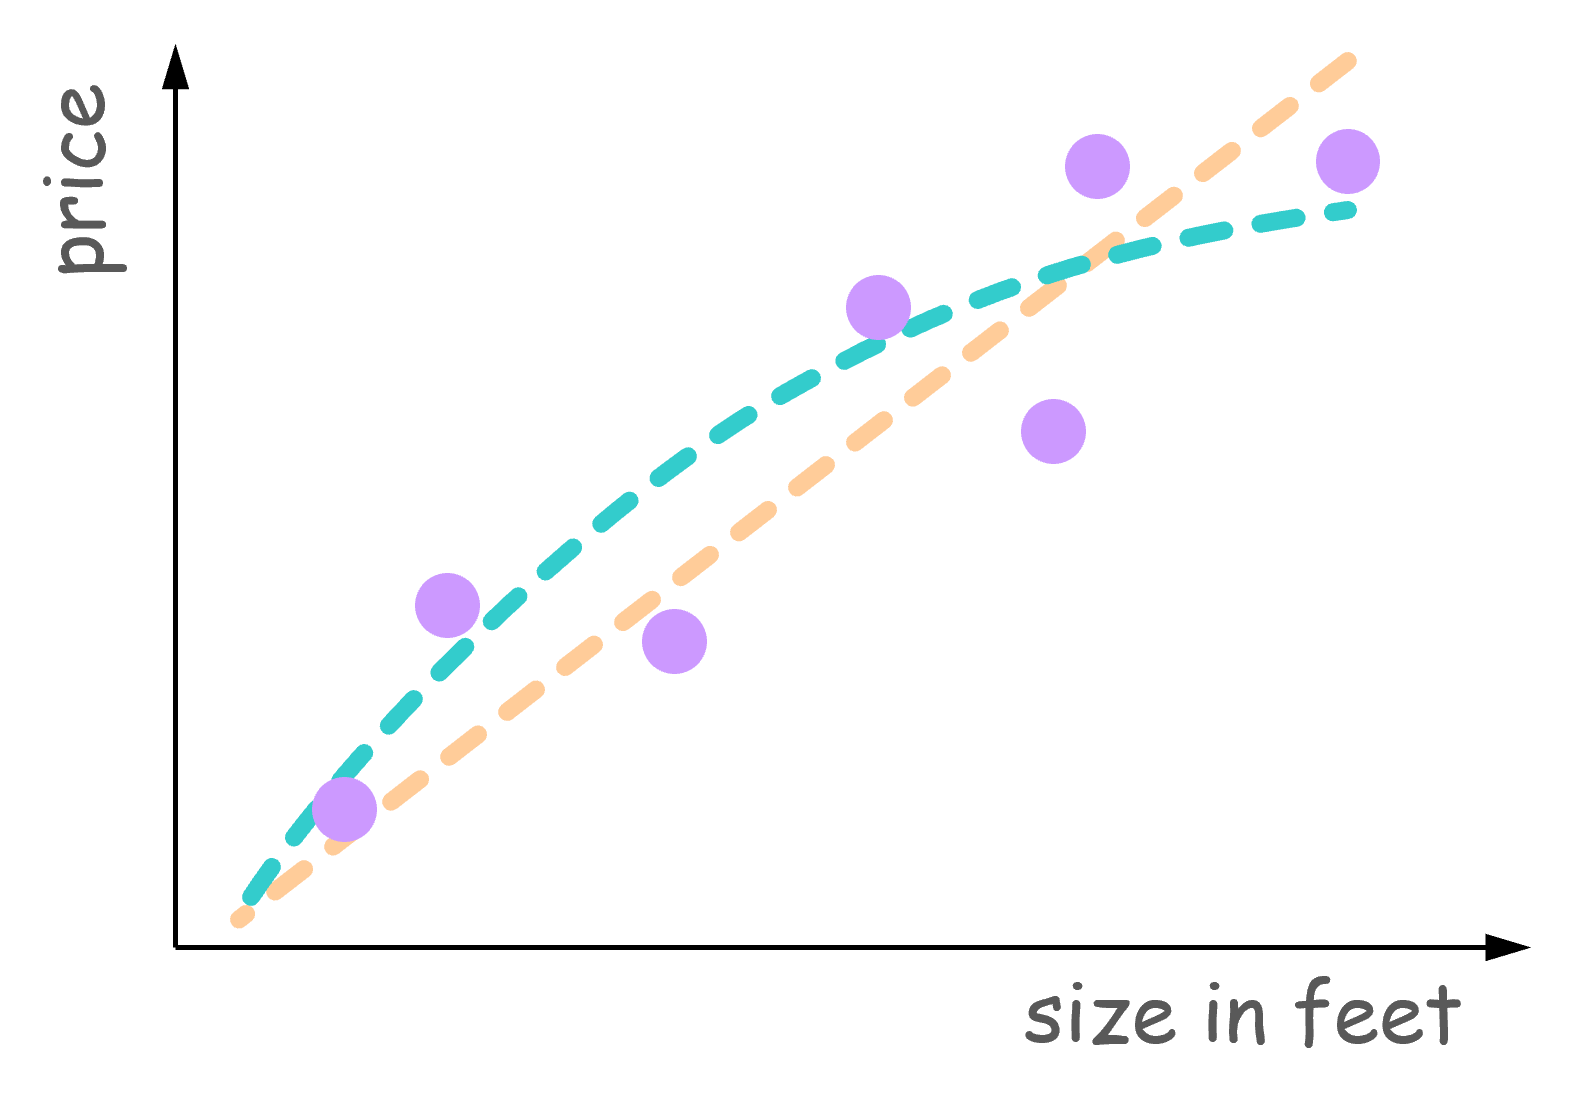
\includegraphics[width=2.4in]{./images/house_price.png}
        \caption{House price}
    \end{minipage}
    \begin{minipage}[t]{0.45\textwidth}
        \centering
        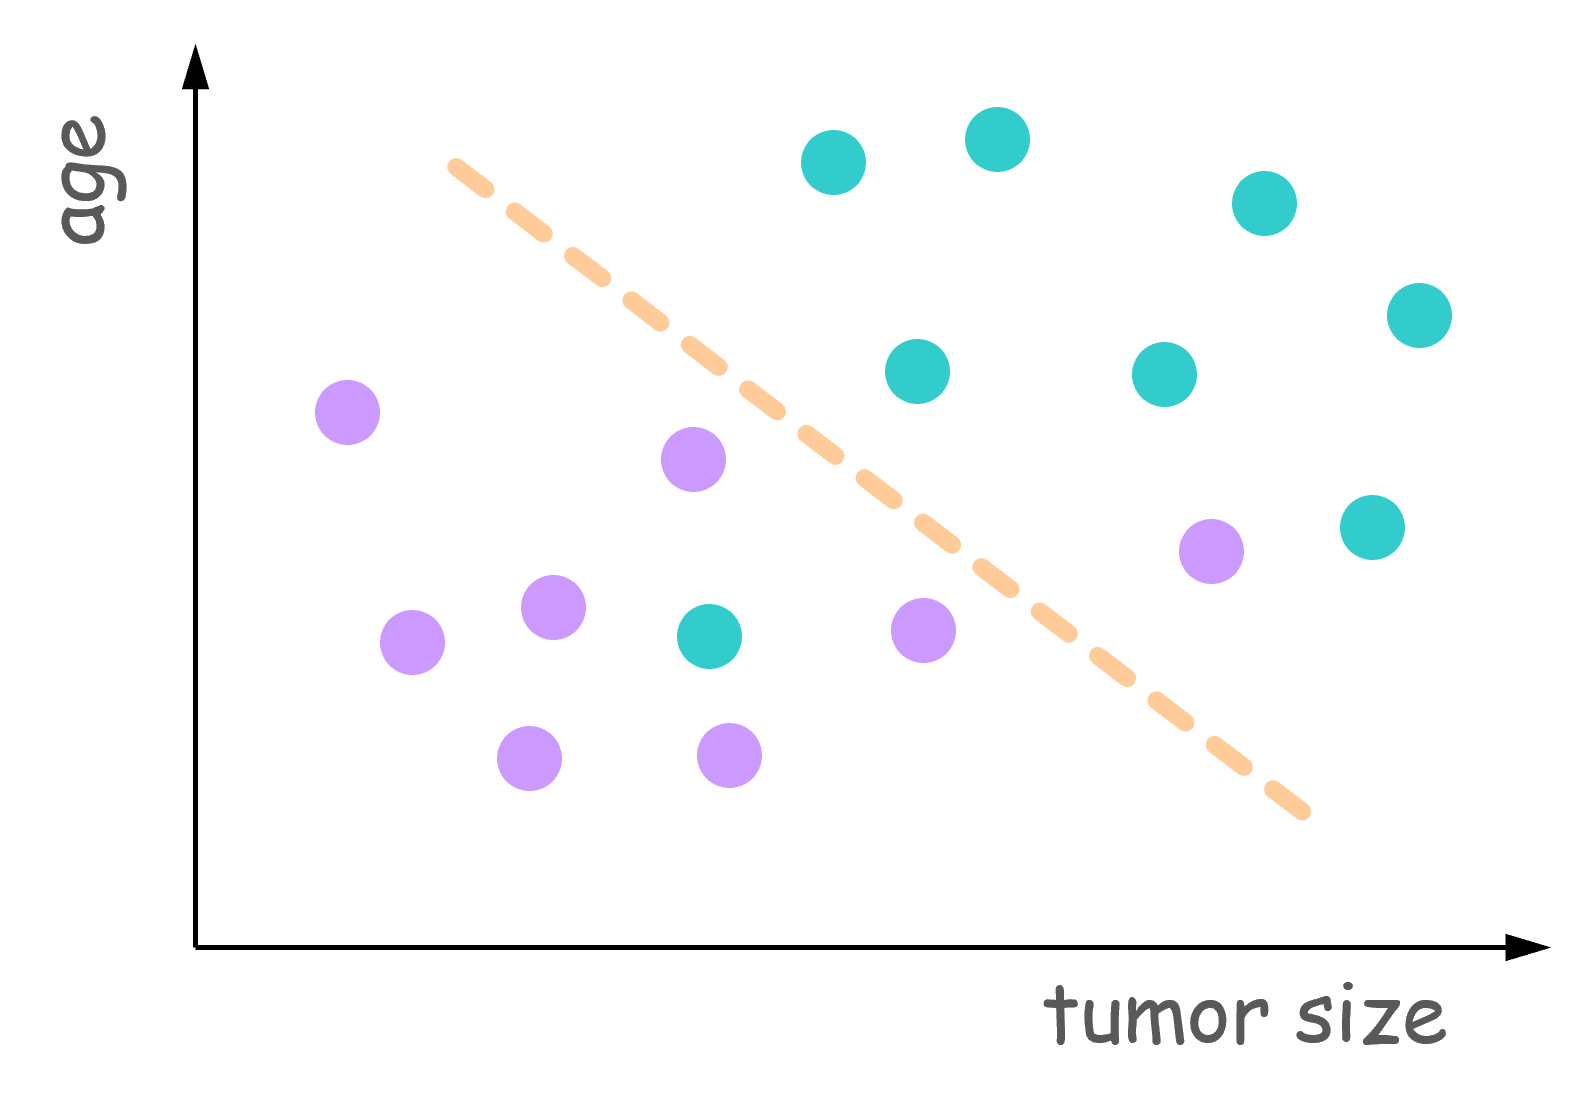
\includegraphics[width=2.4in]{./images/tumor_size.png}
        \caption{Tumor size}
    \end{minipage}
\end{figure}


\section{Unsupervised Learning}
\begin{itemize} 
    \item Approach problems with little or no idea what our results should look like. 
    \item We can derive this structure by clustering the data based on relationships among the variables in the data.
    \item There is no feedback based on the prediction results.
\end{itemize}
\begin{figure}[!htbp]
    \begin{minipage}[t]{0.5\textwidth}
        \centering
        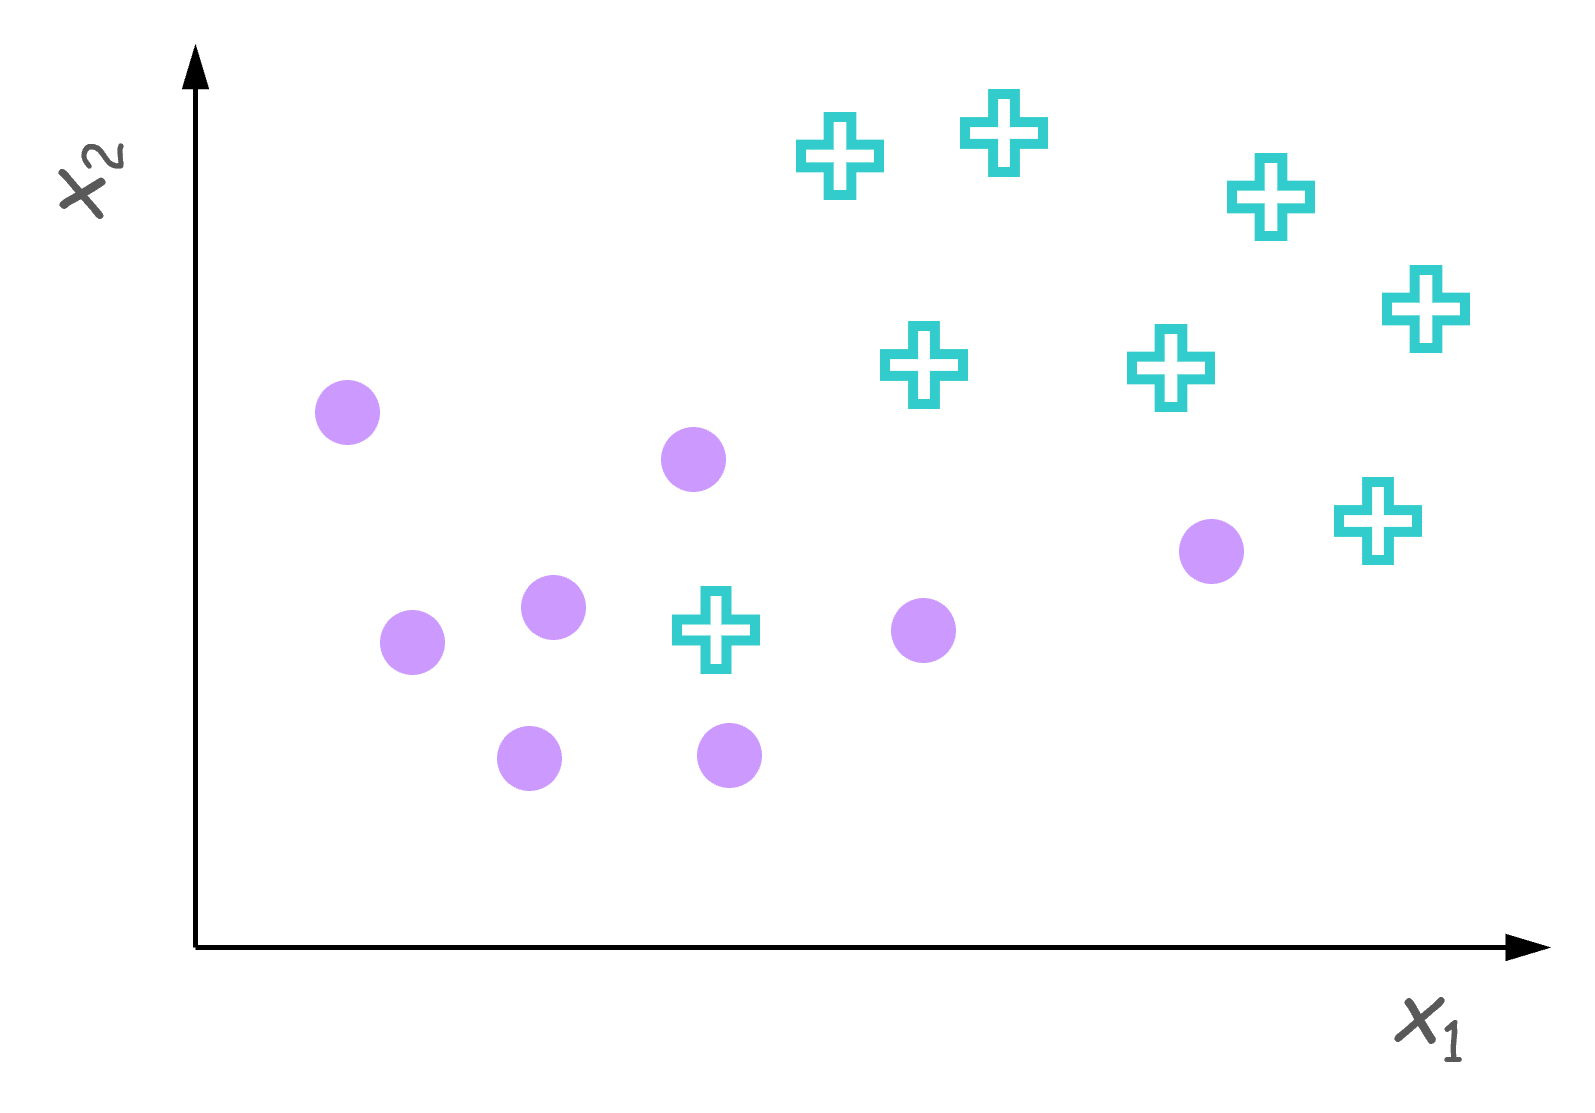
\includegraphics[width=2.0in]{./images/supervised.png}
        \caption{Supervised Learning}
    \end{minipage}
    \begin{minipage}[t]{0.45\textwidth}
        \centering
        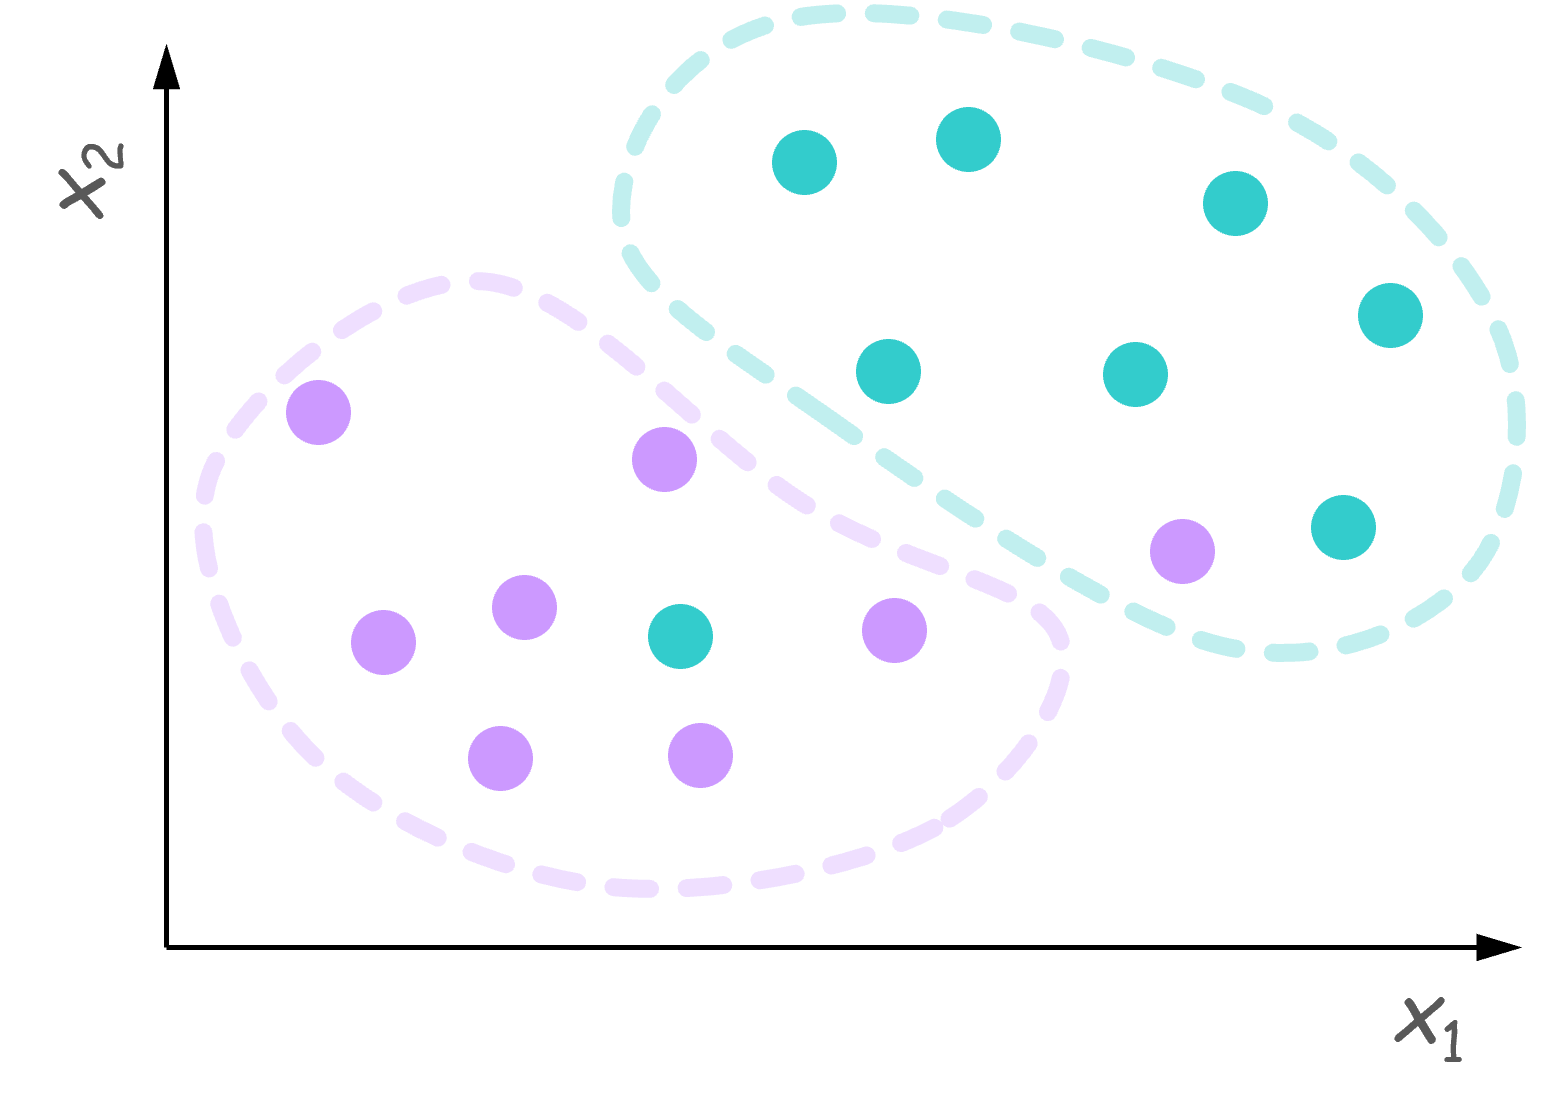
\includegraphics[width=2.0in]{./images/unsupervised.png}
        \caption{Unsupervised Learning}
    \end{minipage}
\end{figure}

    \chapter{Linear Regression}


\section{Introduction}
\begin{itemize} 
    \item Try to predict results using a first-order linear equation \begin{equation} h(x) =  \theta_0 + \theta_1 x \end{equation}
    To make a good prediction, choose appropriate \emph{parameters} $\theta_0$, $\theta_1$ so that $h(x)$ is close to $y$ for our training examples $\left(x, y\right)$
    
    \item Define the cost function \begin{equation} J_\theta\left(\theta_0, \theta_1\right) = \frac{1}{2m}\sum_{i=1}^{m}{\left(h^{(i)}-y^{(i)}\right)^2} \end{equation}
    
    \item The way to choose the parameters is to find \begin{equation} \min_{\theta_0, \theta_1}{J\left(\theta_0, \theta_1\right)} \end{equation}
    Apply \emph{gradient descent method}. Repeat the following until convergence
    \begin{equation} \theta_j \coloneqq \theta_j - \alpha \frac{\partial}{\partial\theta_j}J\left(\theta_0, \theta_1\right) \end{equation} 
    where $j=0, 1$, and $\alpha$ is the learning rate.

    \item If $\alpha$ is too large, it may fail to converge, or even diverge.
    As we approach a local minimum, gradient descent will automatically take smaller steps. So, no need to decrease $\alpha$ over time.
    \begin{figure}[!htbp]
        \centering
        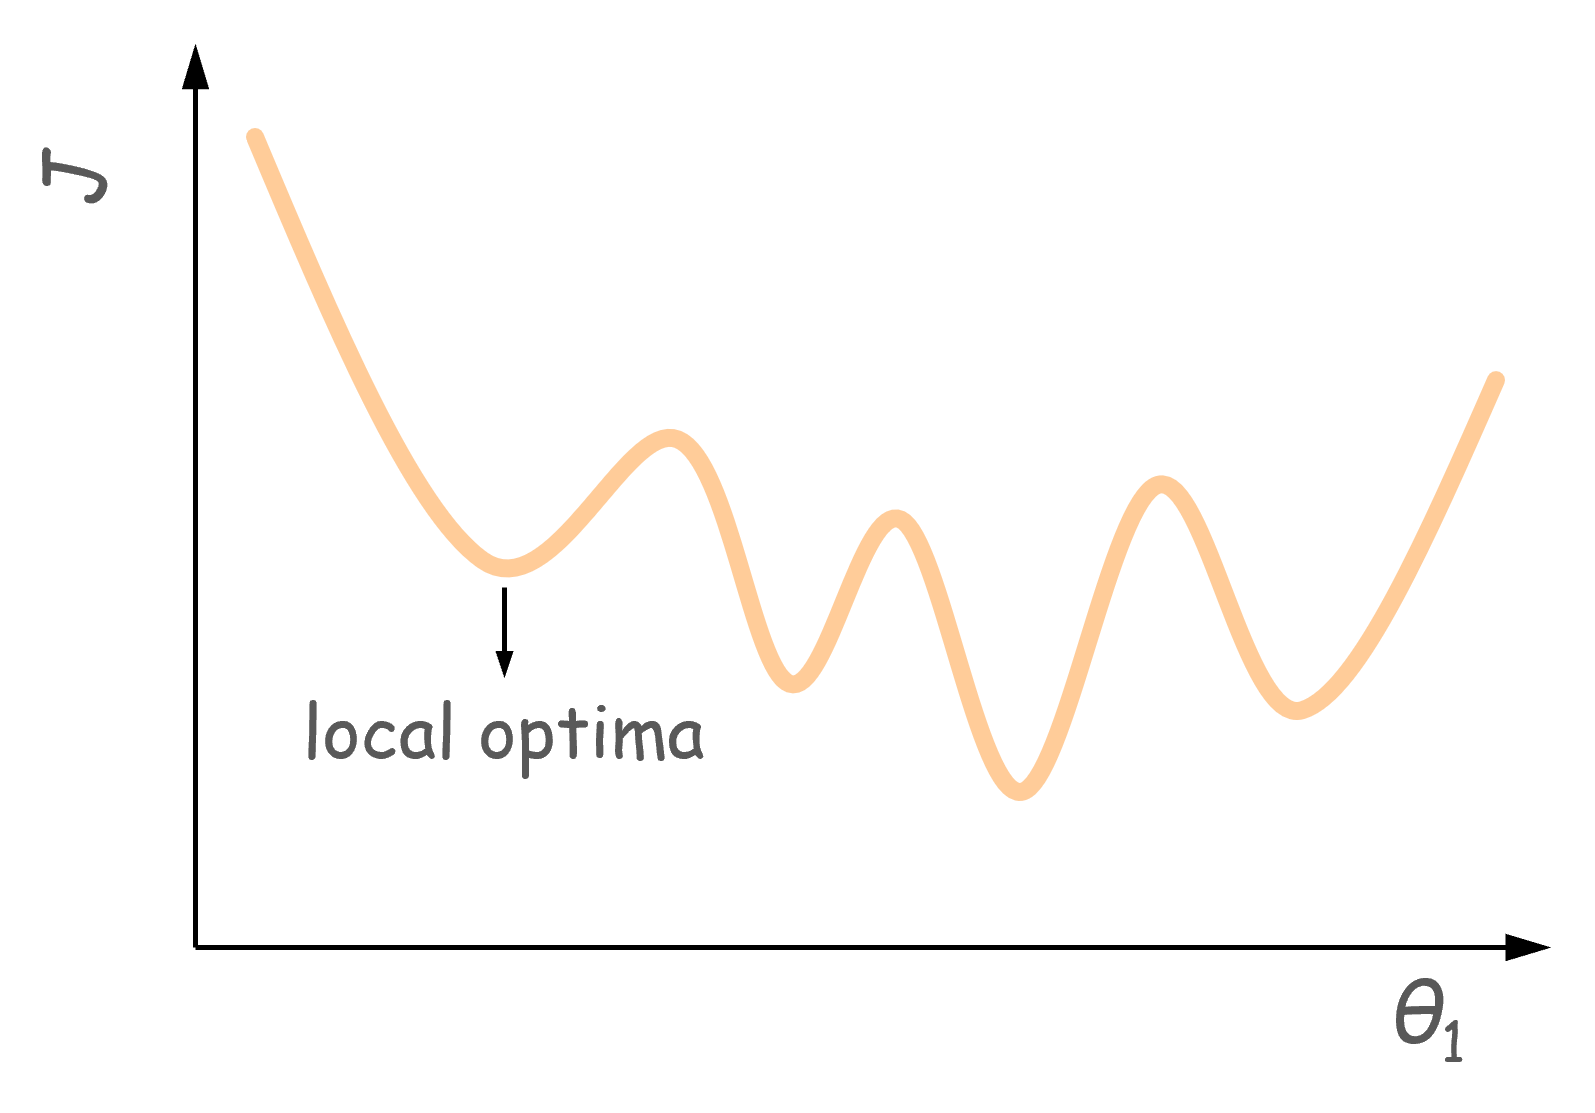
\includegraphics[width=1.8in]{./images/local_optima.png}
        \caption{Local optima}
    \end{figure}
\end{itemize}


\section{Model Representation}
\begin{itemize} 
    \item Assume there are $m$ sets of data and each data has $n$ features, then the raw input could be expressed as a $m \times n$ matrix $\mathbf{X}$:
    \begin{equation}
        \mathbf{X} =
        \left(
        \begin{matrix}
            x_1^{(1)} & x_2^{(1)} & \dots  & x_n^{(1)}\\
            x_1^{(2)} & x_2^{(2)} & \dots  & x_n^{(2)}\\
            \vdots    & \vdots    & \ddots & \vdots   \\
            x_1^{(m)} & x_2^{(m)} & \dots  & x_n^{(m)}\\
        \end{matrix}
        \right)_{m \times n}
    \end{equation}
    
    For polynomial functions, additional features can be created based on $x_1$,
    \begin{equation}
        h\left(x\right) = \theta_0 + \theta_1 x_1 + \theta_2 x_1^2 + \theta_3 x_1^3
    \end{equation}
    Then, the new features could be assumed as $x_2 = x_1^2$, $x_3 = x_1^3$
    
    \item In this course, $\mathbf{X}$ is usually expanded as a $m \times (n+1)$ matrix:
    \begin{equation}
        \mathbf{X} = 
        \left(
        \begin{matrix}
            x_0^{(1)} & x_1^{(1)} & \dots  & x_n^{(1)}\\
            x_0^{(2)} & x_1^{(2)} & \dots  & x_n^{(2)}\\
            \vdots    & \vdots    & \ddots & \vdots   \\
            x_0^{(m)} & x_1^{(m)} & \dots  & x_n^{(m)}\\
        \end{matrix}
        \right)_{m \times (n+1)}
    \end{equation}

    Normally, let $x_0^{(i)} = 1$ so that the first item of the hypothesis would be the constant $\theta_0$ (also called \textbf{bias}). The row component $\mathbf{x}^{(i)}$ of $\mathbf{X}$ means the $i^{th}$ set of training examples
    \footnote{In this document, a component is shown in a normal font such as $x^{(i)}_j$, a vector is shown in a bold font with a lowercase letter such as $\mathbf{x}^{(i)}$, a matrix is shown in a bold font with an uppercase letter such as $\mathbf{X}$.}:
    \begin{equation}
        \mathbf{x}^{(i)} = \left(\begin{matrix} x_0^{(i)} & x_1^{(i)} & \dots & x_n^{(i)} \end{matrix}\right)
    \end{equation}
    
    The columm component $\mathbf{x}_j$ of $\mathbf{X}$ means the $j^{th}$ feature of training examples:
    \begin{equation}
        \mathbf{x}_j = \left(\begin{matrix} x_j^{(1)} \\ x_j^{(2)} \\ \vdots \\ x_j^{(n)} \end{matrix}\right)
    \end{equation}

    \item The multivariable hypothesis function:
    \begin{equation}
        \begin{split}
            h^{(i)} & = \theta_0 x_0^{(i)} + \theta_1 x_1^{(i)} + \theta_2 x_2^{(i)} + \cdots + \theta_n x_n^{(i)}\\
            & = \left[ \begin{matrix} x_0^{(i)} & x_1^{(i)} & x_2^{(i)} & \dots & x_n^{(i)} \end{matrix} \right] 
                \left[ \begin{matrix} \theta_0 \\ \theta_1 \\ \theta_2 \\ \vdots \\ \theta_n \end{matrix} \right] \\
            & = \mathbf{x}^{(i)}\theta
        \end{split}
    \end{equation}                
    
    The relation between the hypothesis $h^{(i)}$ (seemed as \textbf{output}), the \textbf{input} $x_j^{(i)}$ and the \textbf{target} $y^{(i)}$ is:
    \begin{equation}
        \left(
            \begin{matrix}
                h^{(1)} \\
                h^{(2)} \\
                \vdots  \\
                h^{(m)} \\
            \end{matrix}
        \right) =
        \left(
        \begin{matrix}
            1         & x_1^{(1)} & \dots  & x_n^{(1)}\\
            1         & x_1^{(2)} & \dots  & x_n^{(2)}\\
            \vdots    & \vdots    & \ddots & \vdots   \\
            1         & x_1^{(m)} & \dots  & x_n^{(m)}\\
        \end{matrix}
        \right)
        \left(
        \begin{matrix}
            \theta_0\\
            \theta_1\\
            \vdots  \\
            \theta_n\\
        \end{matrix}
        \right)\rightarrow
        \left(
        \begin{matrix}
            y^{(1)} \\
            y^{(2)} \\
            \vdots  \\
            y^{(m)} \\
        \end{matrix}
        \right)
    \end{equation}
\end{itemize}


\section{Cost Function}
\begin{itemize}
    \item Define the cost function and derive a vectorized implementation
    \begin{equation}
        \begin{split}
            J\left(\theta\right)& = \frac{1}{2m}\sum_{i=1}^{m}\left( h^{(i)} - y^{(i)} \right)^2\\
            & = \frac{1}{2m}\sum_{i=1}^{m}\left( \theta_0x_0^{(i)} + \theta_1x_1^{(i)} + \dots + \theta_nx_n^{(i)} - y^{(i)} \right)^2\\
            & = \frac{1}{2m}\sum_{i=1}^{m}\left( \sum_{j=1}^{n}{\theta_j x_j^{(i)}} - y^{(i)} \right)^2\\
            & = \frac{1}{2m}\sum_{i=1}^{m}\left( \mathbf{x}^{(i)}\theta - y^{(i)} \right)^2\\
            & \textcolor{blue}{= \frac{1}{2m}\left( \mathbf{X}\theta - \mathbf{y} \right)\cdot\left( \mathbf{X}\theta - \mathbf{y} \right)}
        \end{split}
    \end{equation}
\end{itemize}
    

\section{Gradient Descent}
\begin{itemize} 

    \item Repeat until convergence
    \begin{equation}
        \begin{split}
            \theta_j& \coloneqq \theta_j - \alpha \frac{\partial}{\partial\theta_j}J\left(\theta\right)\\
                    & \coloneqq \theta_j - \frac{\alpha}{2m} \frac{\partial}{\partial\theta_j} \sum_{i=1}^{m}\left( h^{(i)} - y^{(i)} \right)^2\\
                    & \coloneqq \theta_j - \frac{\alpha}{m} \sum_{i=1}^{m}\left( h^{(i)} - y^{(i)} \right)\left(x_j^{(i)}\right)\\
        \end{split}
    \end{equation}
    for $j=0,1,\dots,n$

    \item In vectorized implementation
    \begin{equation}
        \begin{split}
            \theta & \coloneqq \theta - \frac{\alpha}{m}\mathbf{X}^T\left(\mathbf{X}\theta-\mathbf{y}\right)\\
        \end{split}
    \end{equation}

    \begin{proof}
        Let 
        \begin{equation}
            \nabla_j = \frac{1}{m}\sum_{i=1}^{m}(h^{(i)}-y^{(i)})x_j^{(i)}
        \end{equation}
        
        which is equivalent to
        \begin{equation}
            \nabla_j = \frac{1}{m}(\mathbf{h}-\mathbf{y})^T\mathbf{x}_j
        \end{equation}

        so
        \begin{equation}
            \begin{split}
                \left[ \begin{matrix} \nabla_0 & \nabla_1 & \dots & \nabla_n \end{matrix} \right] &= \frac{1}{m}(\mathbf{h}-\mathbf{y})^T \left[ \begin{matrix} \mathbf{x}_0 & \mathbf{x}_1 & \dots & \mathbf{x}_n \end{matrix} \right]\\
                                                                                                    &= \frac{1}{m}(\mathbf{h}-\mathbf{y})^T \mathbf{X} \\
            \end{split}
        \end{equation}

        thus
        \begin{equation}
            \left[\begin{matrix} \nabla_0 \\ \nabla_1 \\ \vdots \\ \nabla_n \end{matrix}\right] = \left( \frac{1}{m}(\mathbf{h}-\mathbf{y})^T \mathbf{X} \right)^T
                                                                                                = \frac{1}{m} \mathbf{X}^T (\mathbf{h}-\mathbf{y})
        \end{equation}
    \end{proof}

\end{itemize}


\section{Scaling and Normalization}
\begin{itemize} 
    \item We can speed up gradient descent by having each of our input values in roughly the same range. Ideally:
    \begin{equation}
        -1 \leq x^{(i)}_j \leq 1
    \end{equation}
    \item Two techniques to help with this are \textbf{feature scaling} and \textbf{mean normalization}.
    \item \textbf{Feature scaling} involves \textcolor{blue}{dividing} the input values by the range of the input variable, resulting in a new range of just 1.
    \item \textbf{Mean normalization} involves \textcolor{blue}{subtracting} the average value for that input variable resulting in a new average value of just zero. 
    \item To implement both of these techniques, adjust input values as shown in this formula:
    \begin{equation}
        x^{(i)}_j \coloneqq \frac{x^{(i)}_j-\mu^{(i)}}{s^{(i)}}
    \end{equation}
    where $\mu^{(i)}$ is the average of all the values for feature $i$ and $s^{(i)}$ is the range of values, or $s^{(i)}$ is the standard deviation.
\end{itemize}


\section{Normal Equation Method}
\begin{itemize}
    \item This method minimize $J$ by \textbf{explicitly} taking its derivatives with respect to the $\theta_j$, and setting them to zero. The normal equation formula is given below
    \begin{equation}\label{eqn:normal}
        \theta = \left(\mathbf{X}^T\mathbf{X}\right)^{-1}\mathbf{X}^T\mathbf{y}
    \end{equation}
    
    \item If $\left(\mathbf{X}^T\mathbf{X}\right)^{-1}$ is not invertible, the common causes might be having \textbf{redundant features} (i.e. there are linearly dependent features), or \textbf{too many features}  (e.g. $m \leq n$).
    Using \textbf{pinv} function rather than \textbf{inv} when implenting in Octave in this case.
    
    \item
    \begin{proof}
        The derivation of equation \ref{eqn:normal} is presented at \href{https://reurl.cc/0OY4zo}{Eli Bendersky's website}:
        \begin{equation}
            \begin{split}
                J(\theta) &= \frac{1}{2m} \left(\mathbf{X}\theta-\mathbf{y}\right)^{T} \left(\mathbf{X}\theta-\mathbf{y}\right)\\
                                   &= \frac{1}{2m} \left(\theta^{T}\mathbf{X}^{T} - \mathbf{y}^{T}\right) \left(\mathbf{X}\theta-\mathbf{y}\right)\\
                                   &= \frac{1}{2m} \left(\theta^{T}\mathbf{X}^{T}\mathbf{X}\theta - \theta^{T}\mathbf{X}^{T}\mathbf{y} - \mathbf{y}^{T}\mathbf{X}\theta + \mathbf{y}^{T}\mathbf{y}\right)\\
                                   &= \frac{1}{2m} \left(\theta^{T}\mathbf{X}^{T}\mathbf{X}\theta - 2\left(\mathbf{X}\theta\right)^{T}\mathbf{y} + \mathbf{y}^{T}\mathbf{y}\right)
            \end{split}
        \end{equation}
        
        Derive by $\theta$ and compare to 0, $\frac{\partial J}{\partial\theta} = 0$
        \begin{equation}
            \begin{split}
                2\mathbf{X}^T\mathbf{X}\theta - 2\mathbf{X}^T\mathbf{y} = 0\\
                2\mathbf{X}^T\mathbf{X}\theta = 2\mathbf{X}^T\mathbf{y}\\
                \theta = \left(\mathbf{X}^T\mathbf{X}\right)^{-1}\mathbf{X}^T\mathbf{y}
            \end{split}
        \end{equation}
    \end{proof}

    \item The following is a comparison of the algorithmic efficiency between \emph{gradient descent} and \emph{normal equation}
    \begin{table}[H]
        \renewcommand\arraystretch{1.5}
        \caption{Comparison of the algorithmic efficiency}
        \centering
        \begin{tabular}[t]{lll}     
            \hline 
            Items      & Gradient Descent             & Normal Equation          \\ 
            \hline 
            Complexity & $O\left(kn^2\right)$         & $O\left(n^3\right)$      \\ 
            Situation  & Works well when $n$ is large & Slow if $n$ is very large\\
            \hline
        \end{tabular}
    \end{table}
\end{itemize} 

    \chapter{Logistic Regression}


\section{Classification and Hypothesis }
\begin{itemize} 
    \item A \textbf{sigmoid function} is a mathematical function having a characteristic \textbf{s-shaped} curve. A common example of a sigmoid function is the \textbf{logistic function} shown in the figure \ref{fig:sigmoid}.
    \begin{equation}
        g(z) = \frac{1}{1+e^{-z}}
    \end{equation}

    \item When $z \geq 0$, the output will be greater than or equal 0.5.
    \begin{figure}[!htbp]\label{fig:sigmoid}
        \centering
        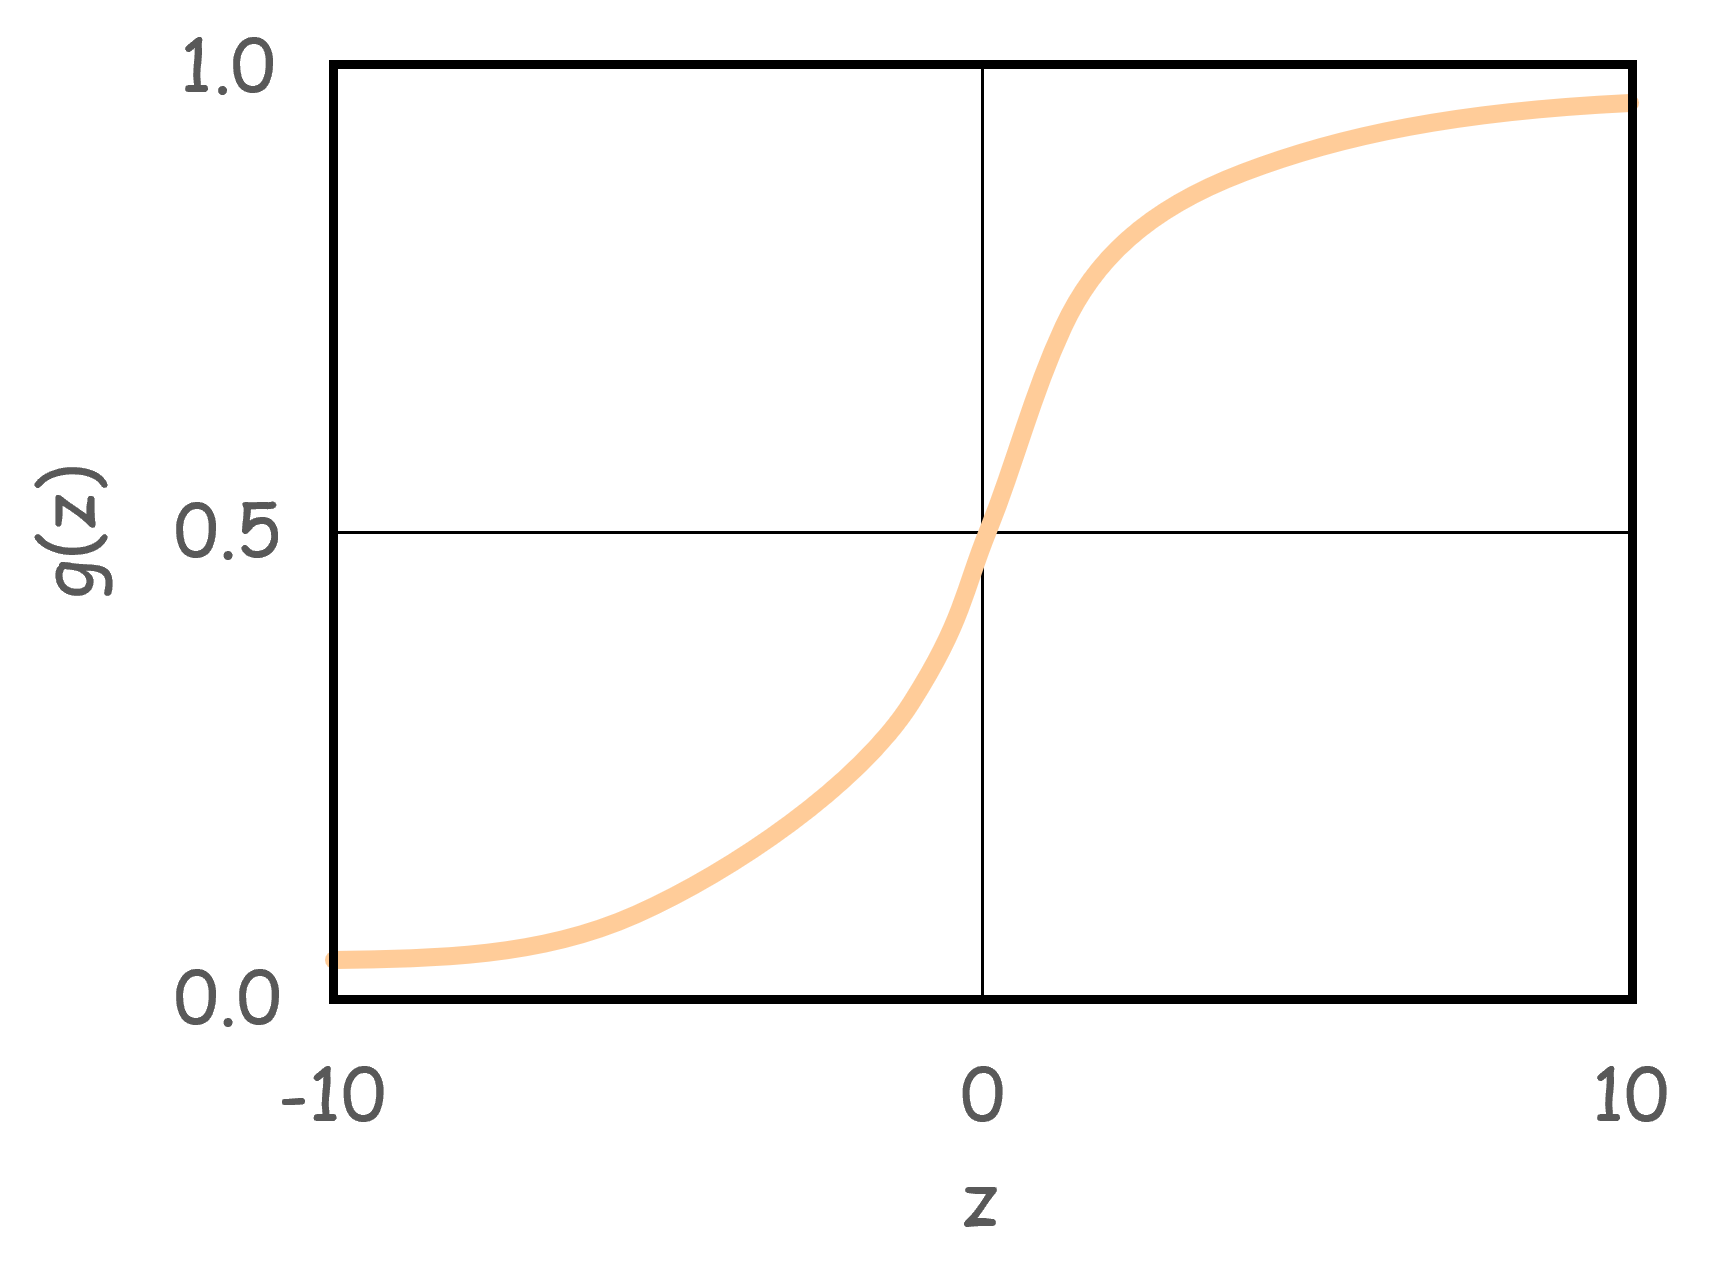
\includegraphics[width=2.8in]{./images/sigmoid.png}
        \caption{Logistic function}
    \end{figure}

    \item For a \textbf{binary classification problem}, $y \in (0,1)$, change the form of the hypothesis  $h^{(i)}$ as a logistic function to satify $0 \leq h^{(i)} \leq 1$. Substitute z into $\mathbf{x}^{(i)}\theta$
    \begin{equation}
        h^{(i)} = \frac{1}{1+e^{-\mathbf{x}^{(i)}\theta}}
    \end{equation}
    where
    \begin{equation}
        \mathbf{x}^{(i)} = 
        \left[
            \begin{array}{cccc}
                x_0^{(i)} & x_1^{(i)} & \dots & x_n^{(i)}  
            \end{array}
        \right],
        \theta = 
        \left[
            \begin{array}{c}
                \theta_0 \\ \theta_1 \\ \vdots \\ \theta_n
            \end{array}
        \right]
    \end{equation}
    Let
    \begin{eqnarray}
        \mathbf{h} = 
        \left[
        \begin{array}{c}
            h^{(1)} \\ h^{(2)} \\ \vdots \\ h^{(m)}
        \end{array}
        \right]
    \end{eqnarray}
    \item The hypothesis $h^{(i)}$ will give the \textbf{probability}. For example, $h^{(i)}=0.7$ means the probability of 70\% that the output is ``1''.
    \begin{equation}
        h^{(i)} = P(y=1|x;\theta) = 1 - P(y=0|x;\theta)
    \end{equation}
\end{itemize}


\section{Cost Function}
\begin{itemize}
    \item If the cost function of a logistic function is used the same as for linear regression, it will cause many local optima. (Not a \textbf{convex} function)
    Instead, the cost function for logistic regression looks like:
    \begin{equation}
        \begin{split}
            J(\theta) = \frac{1}{m}\sum_{i=1}^{m}{L(h^{(i)},y^{(i)})}\\
        \end{split}
    \end{equation}
    
    where,
    \begin{equation}
        L(h^{(i)},y^{(i)}) =
        \left\{
        \begin{array}{ll}
            -\log{(h^{(i)})}   & \mbox{if $y^{(i)}=1$}\\
            -\log{(1-h^{(i)})} & \mbox{if $y^{(i)}=0$}
        \end{array}
        \right.
    \end{equation}
    
    These two cases are shown as Figure \ref{fig:logisticCostttt}. 
    \begin{figure}[!htbp]\label{fig:logisticCostttt}
        \centering
        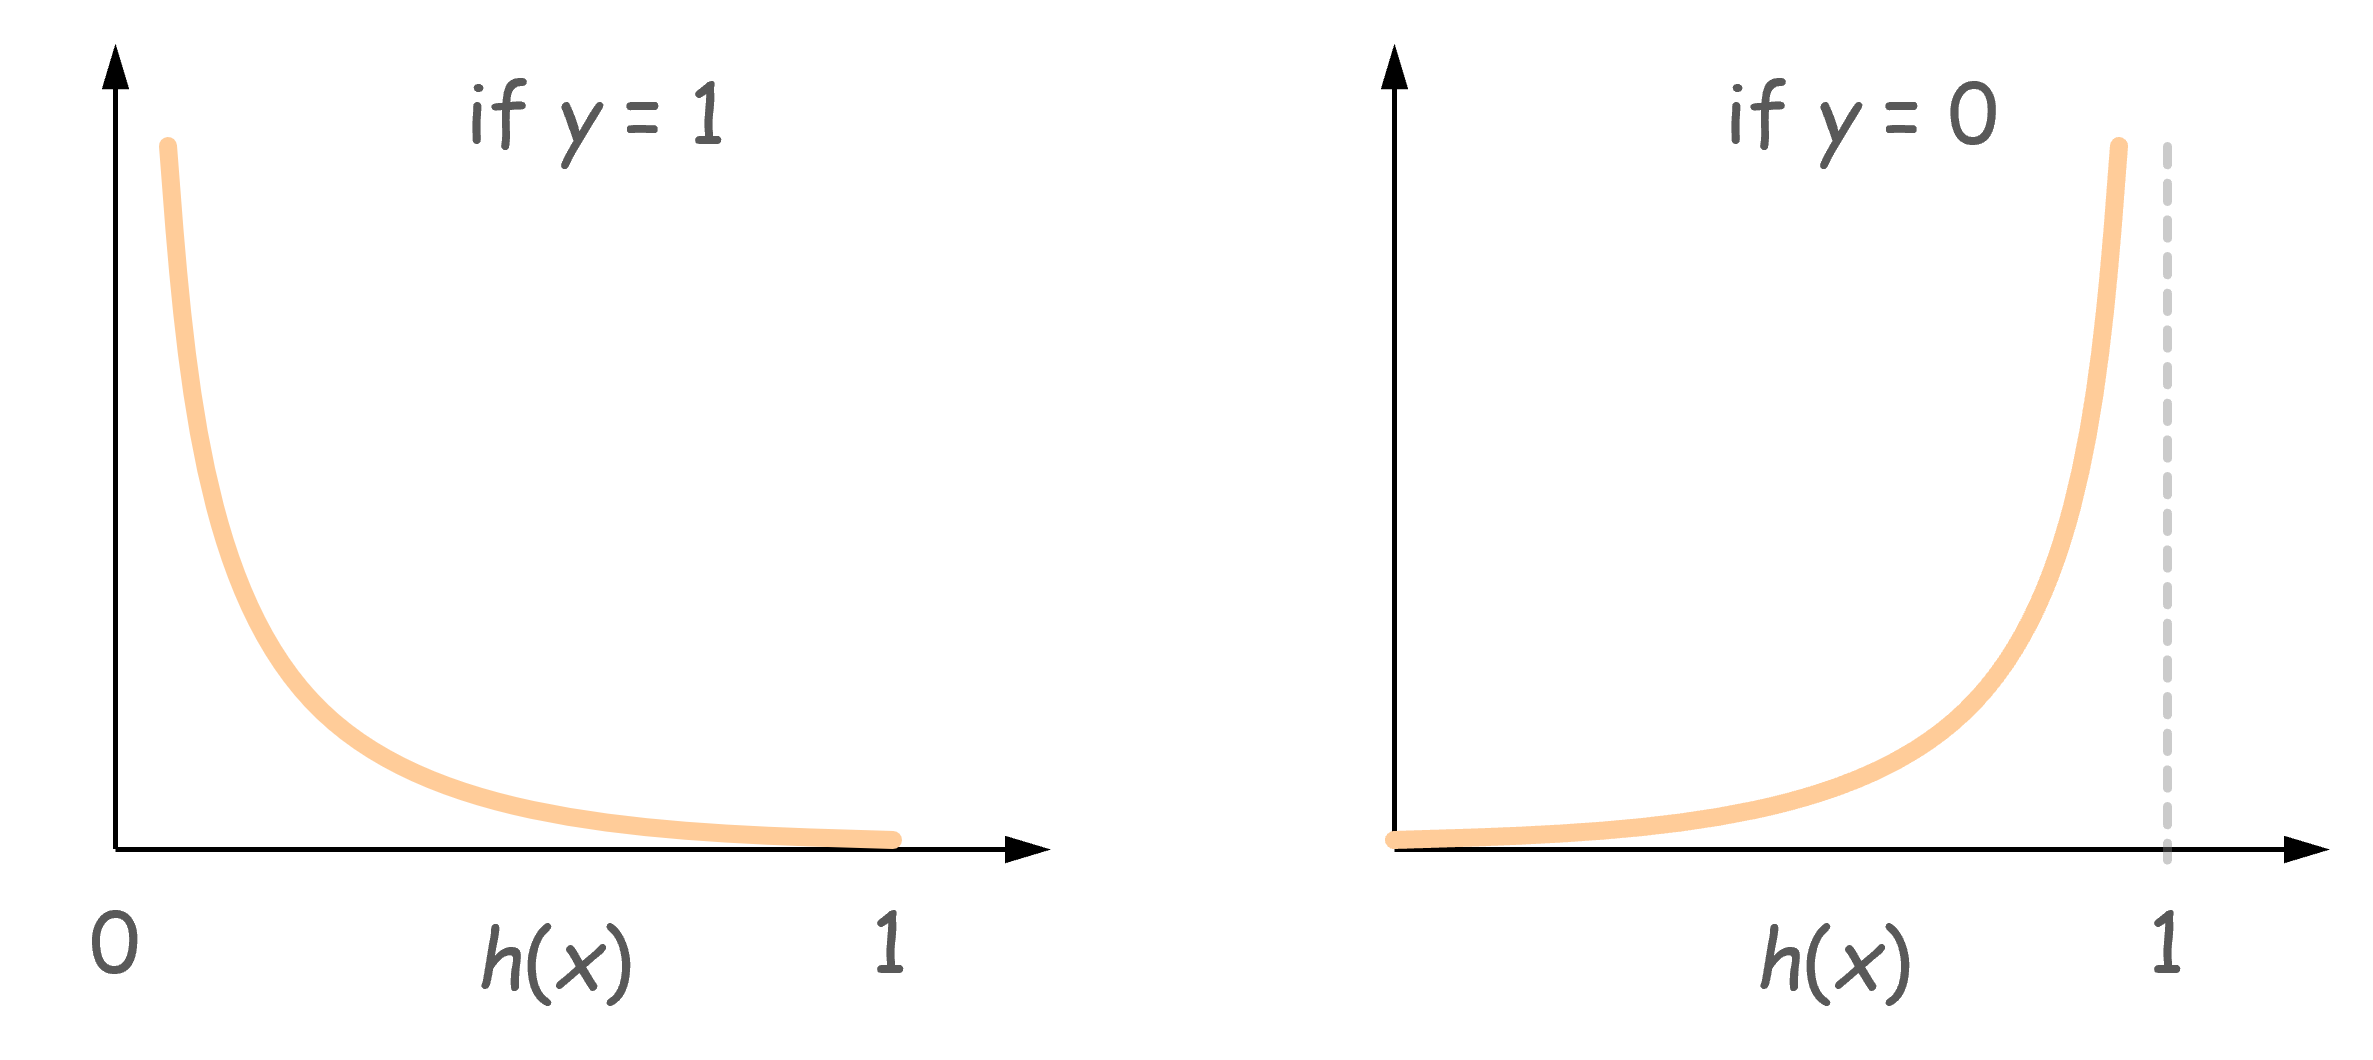
\includegraphics[width=3.2in]{./images/logisticCost.png}
        \caption{Cost of logistic function}
    \end{figure}

    The function $L$ can be compressed into one case
    \begin{equation}
        L(h^{(i)},y^{(i)}) = -y^{(i)}\log{(h^{(i)})}-(1-y^{(i)})\log{(1-h^{(i)})}
    \end{equation}
    
    Thus, the entire cost function as follows:
    \begin{equation}
        J(\theta) = -\frac{1}{m} \sum_{i=1}^{m} \left[ {y^{(i)}\log{(h^{(i)})}+(1-y^{(i)})\log{(1-h^{(i)})}} \right]
    \end{equation}
    
    A vectorized implementation is:
    \begin{equation}
        J(\theta) = -\frac{1}{m} \left( \mathbf{y}^T\log{(\mathbf{h})} + \mathbf{(1-y)}^T\log{(\mathbf{1-h})} \right)
    \end{equation}
\end{itemize}


\section{Gradient Descent}
\begin{itemize}
    \item Repeat until convergence
    \begin{equation}
        \begin{split}
            \theta_j &\coloneqq \theta_j - \alpha \frac{\partial}{\partial\theta_j}J\left(\theta\right)\\
            &\coloneqq \theta_j - \frac{\alpha}{m} \sum_{i=1}^{m}\left[\left(h^{(i)}-y^{(i)}\right)x^{(i)}_j\right]
        \end{split}
    \end{equation}
    for $j=0,1,\dots,n$. 
    \item Surprisingly, the update rule is the same as the one derived in linear regression. As a result, the same gradient descent formula can be used for logistic regression as well.
    
    \item
    \begin{proof}
        The derivative for the cost function is
        \begin{equation}
            \frac{\partial J(\theta)}{\partial\theta_j} = \frac{-1}{m} \sum_{i=1}^{m} \frac{\partial}{\partial h^{(i)}} L\left(h^{(i)},y^{(i)}\right) \frac{\partial h^{(i)}}{\partial \theta_j}
        \end{equation}
        
        Compute the first derivative term, consider the base number of logarithm is $e$
        \begin{equation}
            \begin{split}
                \frac{\partial}{\partial h^{(i)}} L\left(h^{(i)},y^{(i)}\right)  &= y^{(i)} \frac{\partial}{\partial h^{(i)}} \log\left(h^{(i)}\right) + \left(1-y^{(i)}\right) \frac{\partial}{\partial h^{(i)}} \log\left(1-h^{(i)}\right)\\
                &= \frac{y^{(i)}}{h^{(i)}} - \frac{1-y^{(i)}}{1-h^{(i)}}\\
                &= - \frac{h^{(i)}-y^{(i)}}{{h^{(i)}}\left(1-h^{(i)}\right)}
            \end{split}
        \end{equation}
        
        And the second derivative term,
        \begin{equation}
            \begin{split}
                \frac{\partial h^{(i)}}{\partial \theta_j} &= \frac{\partial}{\partial \theta_j} \frac{1}{1+e^{-\mathbf{x}^{(i)}\theta}}
            \end{split}
        \end{equation}
        
        Let
        \begin{equation}
            \begin{split}
                \alpha &= 1 + e^{-\mathbf{x}^{(i)\theta}}\\
                \beta  &= -\mathbf{x}^{(i)}\theta
            \end{split}
        \end{equation}
        
        Then
        \begin{equation}
            \begin{split}
                \frac{\partial h^{(i)}}{\partial \theta_j} &= \frac{\partial h^{(i)}}{\partial \alpha} \frac{\partial \alpha}{\partial \beta} \frac{\partial \beta}{\partial \theta_j}\\
                &= \frac{-1}{\left(1 + e^{-\mathbf{x}^{(i)\theta}}\right)^2} e^{-\mathbf{x}^{(i)\theta}} \left(-x^{(i)}_j\right)\\
                &= \frac{1}{1+e^{-\mathbf{x}^{(i)\theta}}} \left(\frac{-e^{-\mathbf{x}^{(i)\theta}}}{1+e^{-\mathbf{x}^{(i)\theta}}}\right)\left(-x^{(i)}_j\right)\\
                &= h^{(i)} \left(1-h^{(i)}\right) \left(-x^{(i)}_j\right)
            \end{split}
        \end{equation}
        
        So
        \begin{equation}
            \frac{\partial J(\theta)}{\partial\theta_j} = \frac{-1}{m} \sum_{i=1}^{m} \left[\left(h^{(i)}-y^{(i)}\right)x^{(i)}_j\right]
        \end{equation}
    \end{proof}

    \item The vectorized implementation is
    \begin{equation}
        \mathbf{\theta} \coloneqq \mathbf{\theta} - \frac{\alpha}{m}\mathbf{X}^T\left(\mathbf{h}-\mathbf{y}\right)
    \end{equation}


\end{itemize}


\section{Decision Boundary}
\begin{itemize}
    \item After the optimization of parameters $\theta_j$ where $j=0,\dots,n$, the decision boundary is
    \begin{equation}
        \theta_0 x_0 + \theta_1 x_1 + \dots + \theta_n x_n = 0
    \end{equation}
    
    \item For example. If
    \begin{equation}
        \theta = 
        \left[\begin{array}{ccc} -3 & 1 & 1 \end{array}\right]^T
    \end{equation}
    
    The decision boundary is
    \begin{equation}
        -3 x_0 + x_1 + x_2 = 0
    \end{equation}

    For those points located at the upper-right side of the decision boundary, the predictions are $y=1$.
    On the contrary, for those points located at the lower-left side are $y=0$.
    \begin{figure}[!htbp]
        \centering
        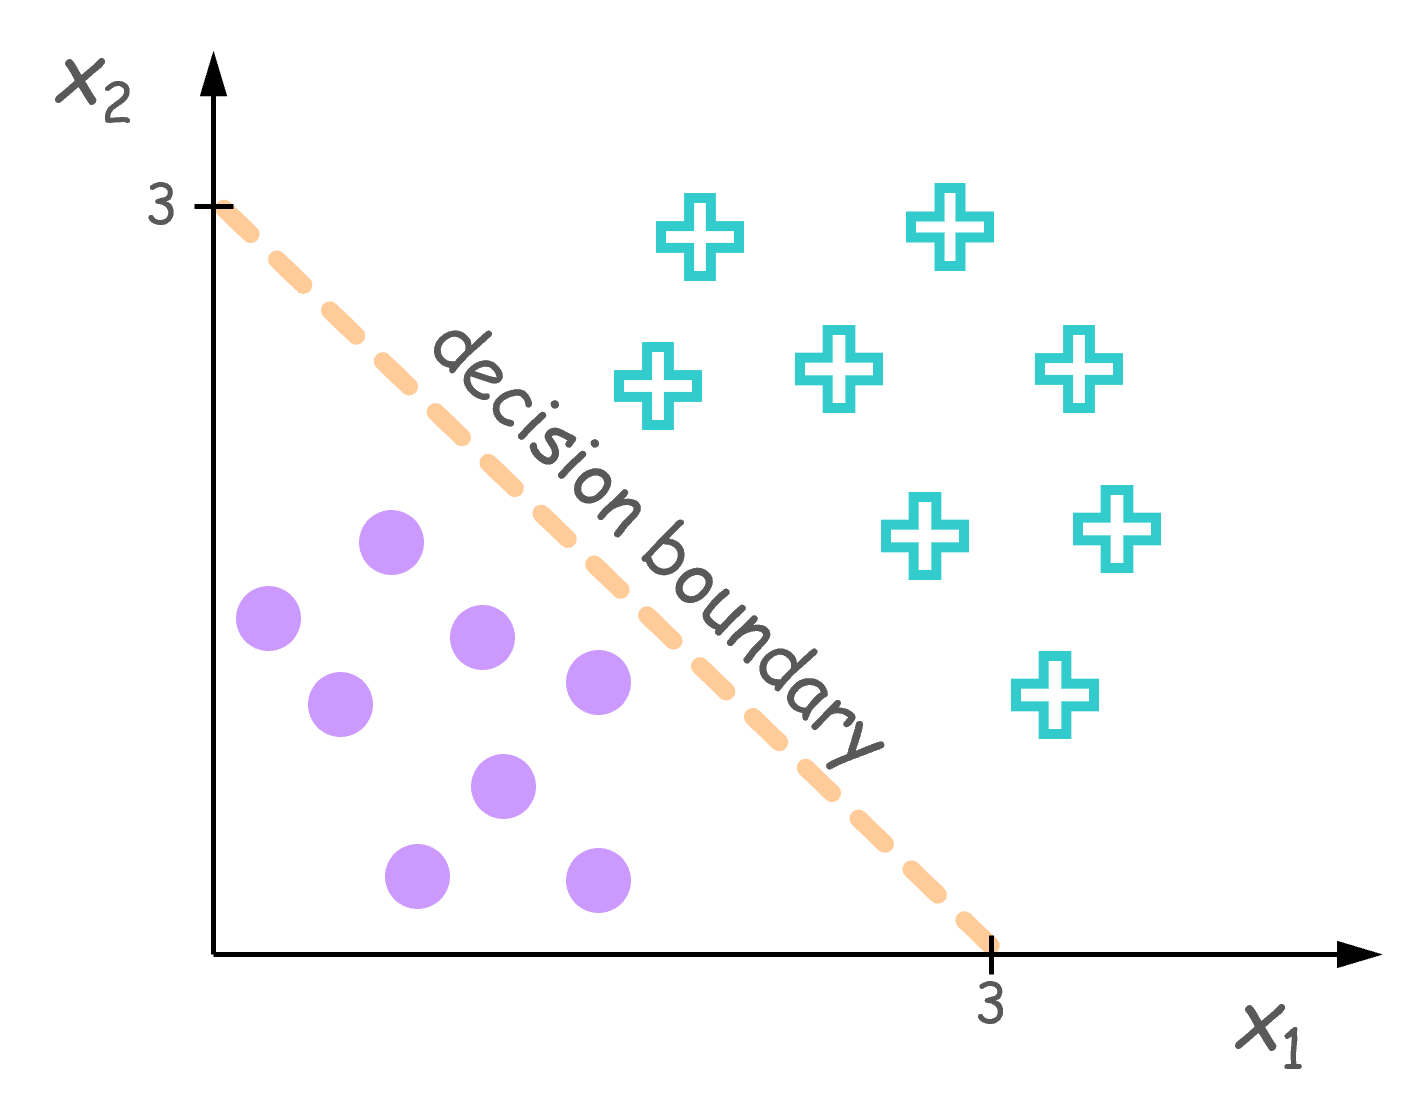
\includegraphics[width=2.6in]{./images/decision boundary.png}
        \caption{Logistic function}
    \end{figure}
    
    \item An non-linear decision boundary can also be created by adding polynomial terms in the array of parameters, such as
    \begin{equation}
        \theta = 
        \left[\begin{array}{ccccc} \theta_0 & \theta_1 & \theta_2 & \theta_1^2 & \theta_2^2 \end{array}\right]^T
    \end{equation}
    
    For this case, the optimized parameters would be like
    \begin{equation}
        \theta = 
        \left[\begin{array}{ccccc} -1 & 0 & 0 & 1 & 1 \end{array}\right]^T
    \end{equation}
    
    Then the decision boundary is
    \begin{equation}
        -1 + x_1^2 + x_2^2 = 0
    \end{equation}

    The prediction would be
    \begin{equation}
        y = \left\{\begin{aligned}
            1 &\text{, for } x_1^2 + x_2^2 \geq 1\\
            0 &\text{, for } x_1^2 + x_2^2 < 1
        \end{aligned}\right.
    \end{equation}

    \begin{figure}[!htbp]
        \centering
        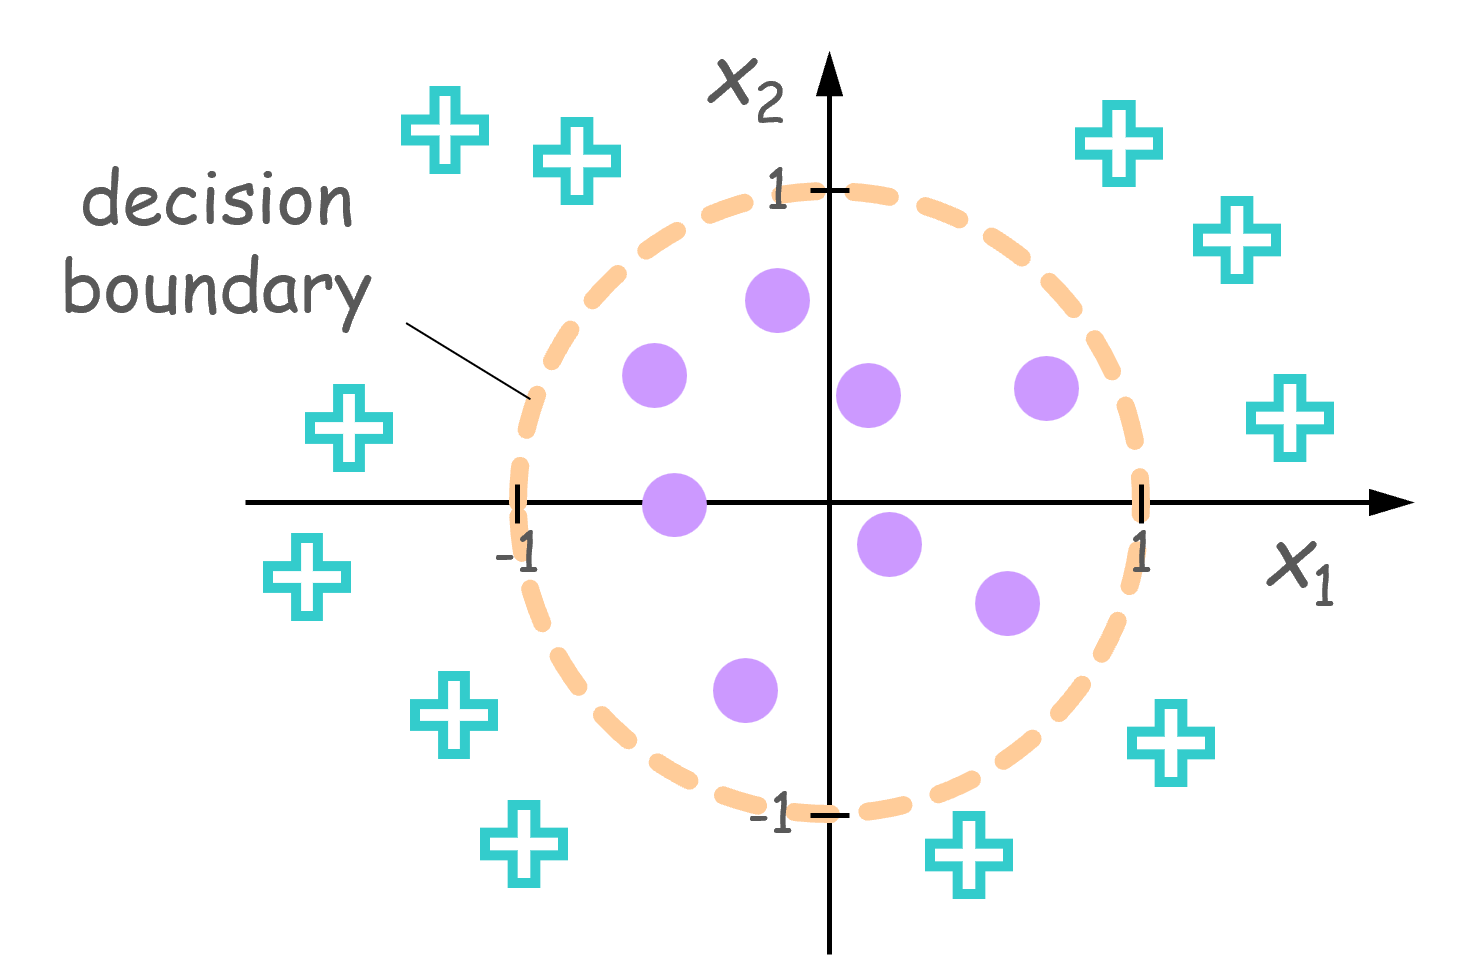
\includegraphics[width=2.6in]{./images/decision boundary_nonlinear.png}
        \caption{Logistic function}
    \end{figure}
    
\end{itemize}
    \chapter{Regularization}


\section{Overfitting}
\begin{itemize}
    \item The hypothesis in Figure \ref{fig:overfitting} are:
        \begin{itemize}
            \item $h(x) = \theta_0 + \theta_1x \Rightarrow$ underfitting
            \item $h(x) = \theta_0 + \theta_1x + \theta_2x^2$
            \item $h(x) = \theta_0 + \theta_1x + \theta_2x^2 + \theta_3x^3 + \theta_4x^4 \Rightarrow$ overfitting
        \end{itemize}
    \begin{figure}[!htbp]\label{fig:overfitting}
        \centering
        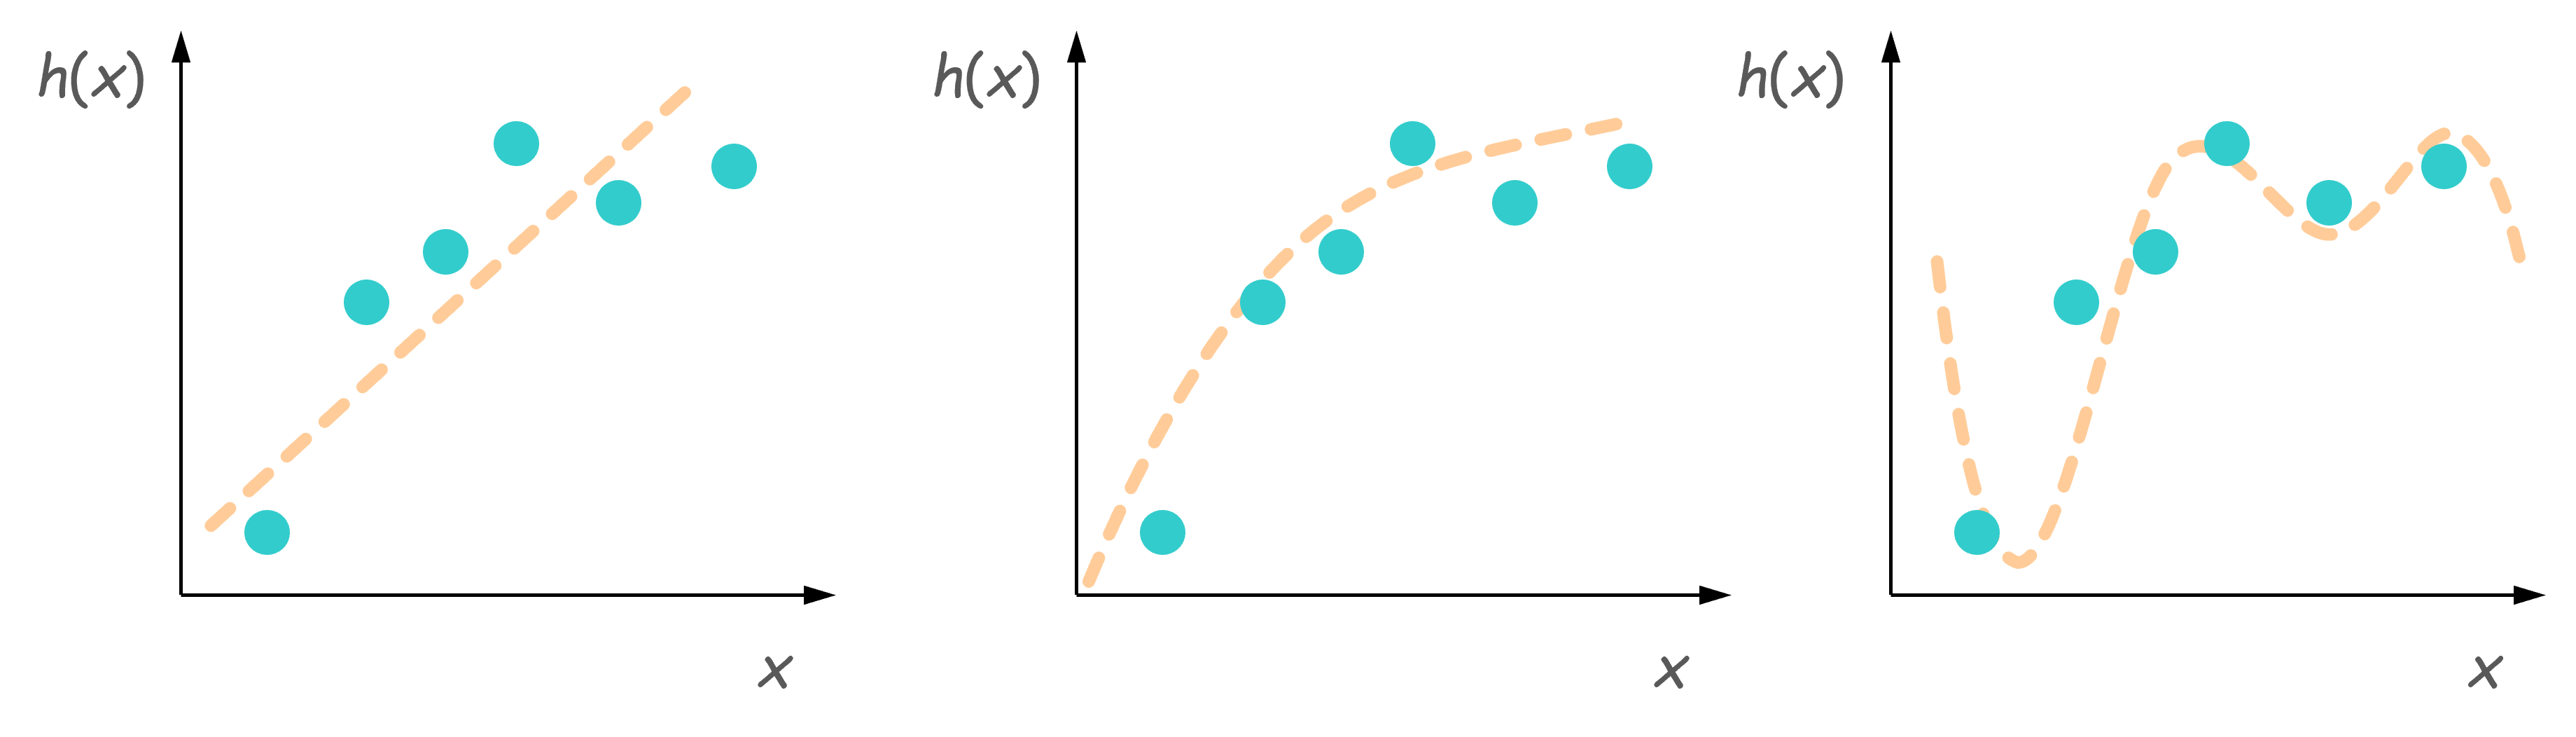
\includegraphics[width=5.4in]{./images/overfitting.png}
        \caption{Three different regression models}
    \end{figure}
    Two main options to address these issue, \textbf{reducing features} and \textbf{regularization}.
    
    \item \textbf{Reduce the number of features}
        \begin{itemize}
            \item Manually select
            \item Use a model selection algorithm
        \end{itemize}
    \item \textbf{Regularization}
        \begin{itemize}
            \item Keep all the features, but reduce the magnitude of parameters $\theta_j$
            \item Works well when slightly features are useful.
        \end{itemize}
\end{itemize}


\section{Regularized Linear Regression}
\begin{itemize}
    \item The intuition of regularization is shown as \ref{fig:intuitionRegularization}
    \begin{figure}[H]\label{fig:intuitionRegularization}
        \centering
        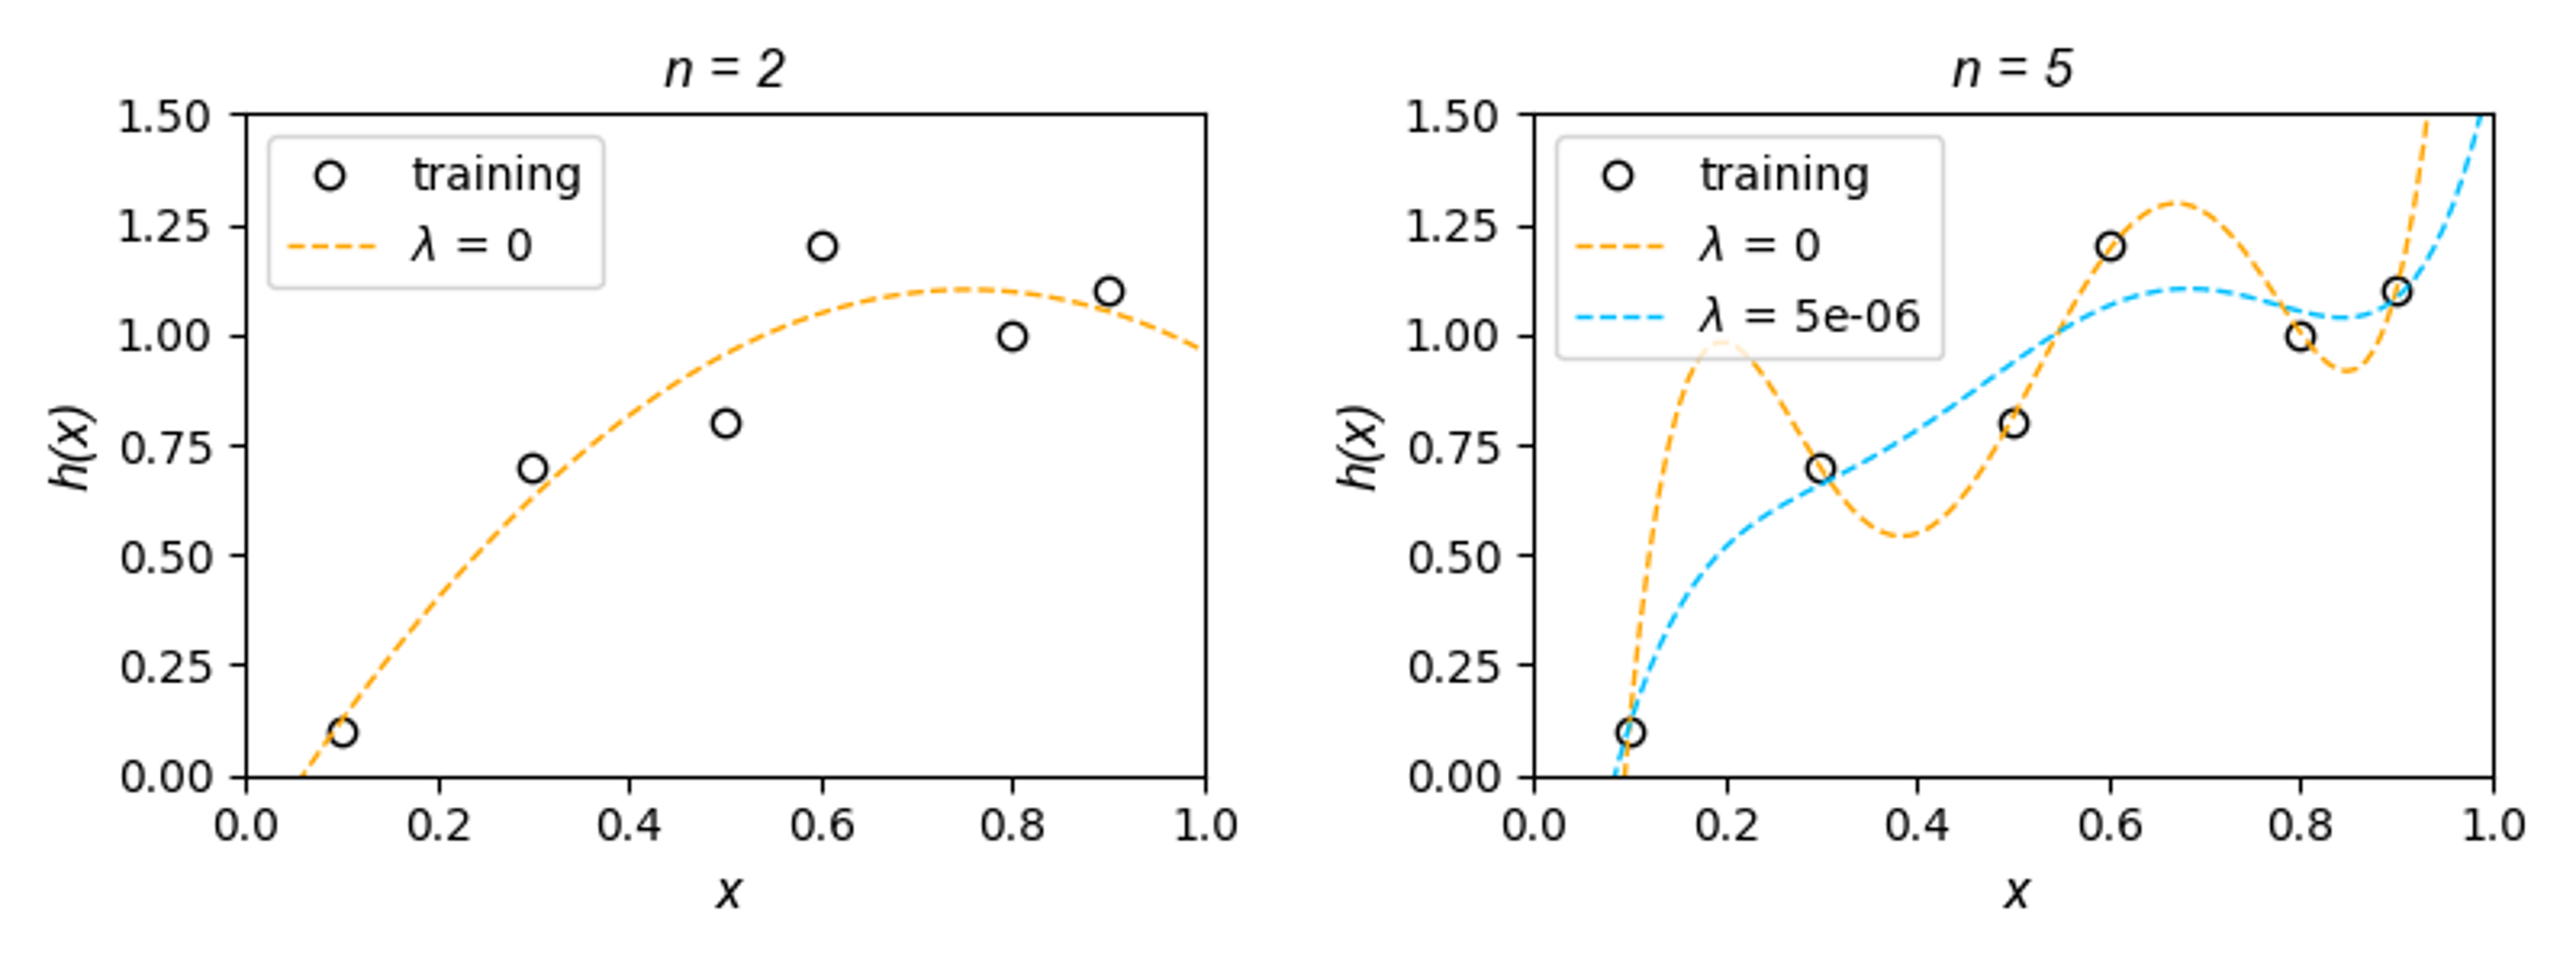
\includegraphics[width=5.4in]{./images/intuitionRegularization.png}
        \caption{The intuition of regularization}
    \end{figure}
    
    \item A regularization term (or regularizer) $\sum_{j=1}^{n}{\theta_j^2}$ is added to the cost function to impose a penalty on the complexity of $h^{(i)}$.
    \begin{equation}\label{eqn:regularCostLinear}
        J(\theta) = \frac{1}{2m} \left[ \sum_{i=1}^{m} { (h^{(i)} - y^{(i)})^2} + \lambda \sum_{j=1}^{n}{\theta_j^2} \right]
    \end{equation}
    The $\mathbf{\lambda}$ is the regularization parameter which controls the importance of the regularization term.
    To reduce the function variety, only the higher-order terms would be penalized, so $\theta_0$ is excluded from the regularization term.

    \item The way to choose the parameters is to find \begin{equation} \min_{\theta}{J\left(\theta\right)} \end{equation}
    Because the regularization term is add to the cost function, the minimization process would not find out the optimum which make $h^{(i)}$ closest to $y^{(i)}$.
    The errors between each $h^{(i)}$ and $y^{(i)}$ would be bigger, so the shape of function would not be too \emph{overfitting}.

    \item To prevent penalize $\theta_0$, it is separated out from the rest of parameters of \textbf{gradient descent} function. 
    \begin{equation}
        \left\{
        \begin{aligned}
            \theta_0 &\coloneqq \theta_0 - \frac{\alpha}{m} \sum_{i=1}^{m} {\left(h^{(i)} - y^{(i)}\right)x_0^{(i)}}\\
            \theta_j &\coloneqq \theta_j - \frac{\alpha}{m} \sum_{i=1}^{m} \left[ {\left( h^{(i)} - y^{(i)}\right)x_j^{(i)} + \lambda\theta_j} \right]\\
        \end{aligned}
        \right.
    \end{equation}
    for $j = 1, \dots, n$ and $j \neq 0$. The vectorized implementation would be
    \begin{equation}
        \mathbf{\theta} \coloneqq \mathbf{\theta} - \frac{\alpha}{m} \left[ \mathbf{X}^T \left(\mathbf{h} - \mathbf{y}\right) + \lambda\mathbf{L}\mathbf{\theta} \right]
    \end{equation}
    where
    \begin{equation}
        \mathbf{L} = 
        \left[
        \begin{matrix}
            0      &        &        &        &       \\
                   & 1      &        &        &       \\
                   &        & 1      &        &       \\
                   &        &        & \ddots &       \\
                   &        &        &        & 1     \\
        \end{matrix}
        \right]
    \end{equation}
    \item And the regularized \textbf{normal equation} becomes
    \begin{equation}\label{eqn:normalRegularized}
        \begin{split}
            \mathbf{\theta} = \left(\mathbf{X}^T\mathbf{X} + \lambda \mathbf{L}\right)^{-1}\mathbf{X}^T\mathbf{y}\\
        \end{split}
    \end{equation}

    Recall that if $m<n$, then $\mathbf{X}^T\mathbf{X}$ is non-invertible. However, when we add the term $\lambda\mathbf{L}$, then $\mathbf{X}^T\mathbf{X} + \lambda\mathbf{L}$ becomes invertible.
    \begin{proof}
        \begin{equation}
            \begin{split}
                J(\mathbf{\theta}) &= \frac{1}{2m} \left[ \left(\mathbf{X}\mathbf{\theta}-\mathbf{y}\right)^{T}\left(\mathbf{X}\mathbf{\theta}-\mathbf{y}\right) + \lambda\mathbf{\theta}^T\mathbf{L}\mathbf{\theta} \right]\\
                                   &= \frac{1}{2m} \left[ \mathbf{\theta}^{T}\mathbf{X}^{T}\mathbf{X}\mathbf{\theta} - 2\left(\mathbf{X}\mathbf{\theta}\right)^{T}\mathbf{y} + \mathbf{y}^{T}\mathbf{y} + \lambda\mathbf{\theta}^T\mathbf{L}\mathbf{\theta} \right]
            \end{split}
        \end{equation}

        Derive by $\mathbf{\theta}$ and compare to 0, $\frac{\partial J}{\partial\mathbf{\theta}} = 0$
        \begin{equation}
            \begin{split}
                2\mathbf{X}^T\mathbf{X}\mathbf{\theta} - 2\mathbf{X}^T\mathbf{y} + 2\lambda\mathbf{L}\mathbf{\theta}= 0\\
                (\mathbf{X}^T\mathbf{X} + \lambda\mathbf{L})\mathbf{\theta} = \mathbf{X}^T\mathbf{y}\\
                \mathbf{\theta} = \left(\mathbf{X}^T\mathbf{X} + \lambda\mathbf{L}\right)^{-1}\mathbf{X}^T\mathbf{y}
            \end{split}
        \end{equation}
    \end{proof}
\end{itemize}


\section{Regularized Logistic Regression}
\begin{itemize}
    \item The way to regularize a logistic regression is similar to linear regression.
    \begin{figure}[H]\label{fig:logisticFit}
        \centering
        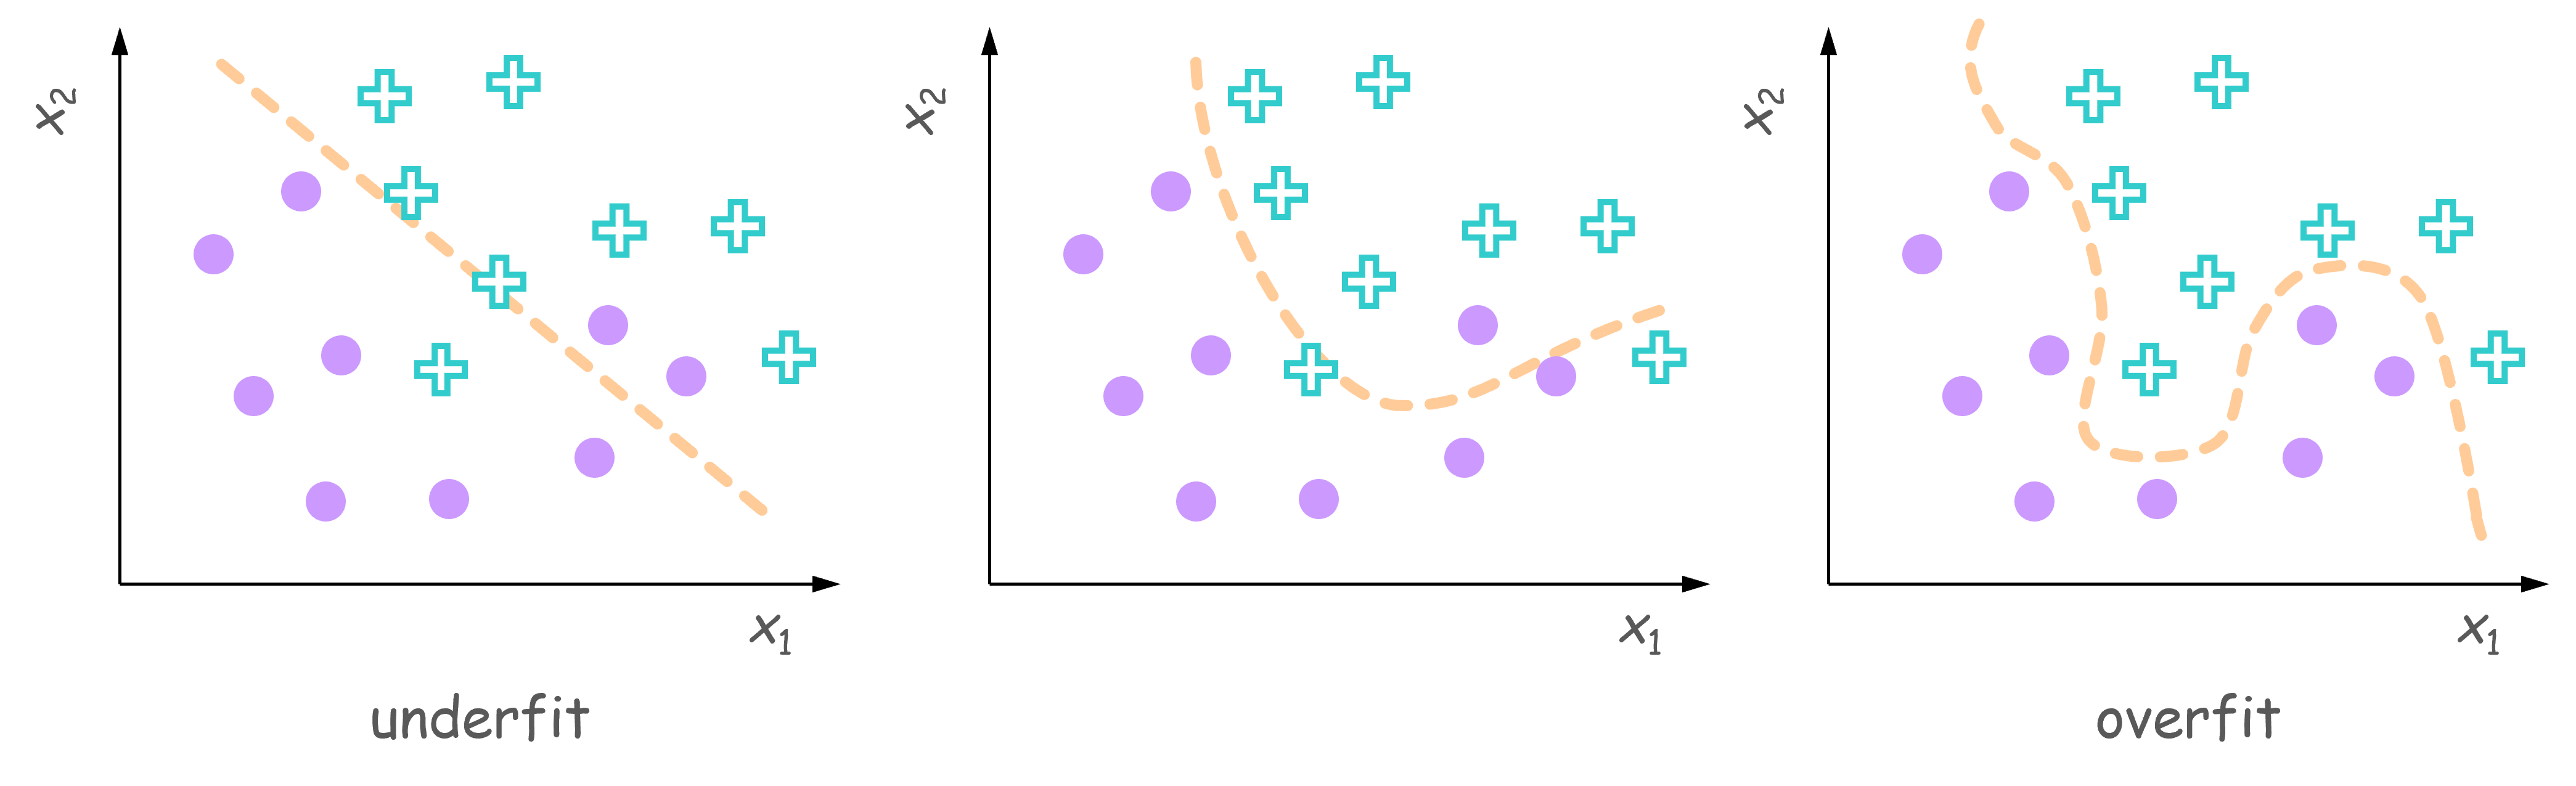
\includegraphics[width=5.4in]{./images/logisticFit.png}
        \caption{Three different regression models}
    \end{figure}
    
    \item Define the cost function
    \begin{equation}
        J(\mathbf{\theta}) = \frac{-1}{m}\sum_{i=1}^{m}{\left[y^{(i)} \log{(h^{(i)})} + (1-y^{(i)}) \log{(1-h^{(i)})} \right]} + \frac{\lambda}{2m}\sum_{j=1}^{n}{\theta_j^2}
    \end{equation}
    The regularization term is added and it is the same as which in (\ref{eqn:regularCostLinear}).
    
    \item Gradient descent
    \begin{equation}
        \left\{
        \begin{aligned}
            \theta_0 &\coloneqq \theta_0 - \frac{\alpha}{m} \sum_{i=1}^{m} {\left(h^{(i)} - y^{(i)}\right)x_0^{(i)}}\\
            \theta_j &\coloneqq \theta_j - \frac{\alpha}{m} \sum_{i=1}^{m} \left[ {\left( h^{(i)} - y^{(i)}\right)x_j^{(i)} + \lambda\theta_j} \right]\\
        \end{aligned}
        \right.    
    \end{equation}
    for $j = 1, \dots, n$ and $j \neq 0$. The vectorized implementation would be
    \begin{equation}
        \mathbf{\theta} \coloneqq \mathbf{\theta} - \frac{\alpha}{m} \left[ \mathbf{X}^T \left(\mathbf{h} - \mathbf{y}\right) + \lambda\mathbf{L}\mathbf{\theta} \right]
    \end{equation}
\end{itemize}
    
    \chapter{Neural Networks}


\section{Model Representation}
\begin{itemize}
    \item Neural networks were developed as simulating neurons or networks of neurons in the brain.
    \item Neurons are basically computational units that take inputs (dendrites) as electrical inputs (called ``spikes'') that are channeled to outputs (axons).
    \begin{figure}[H]
        \centering
        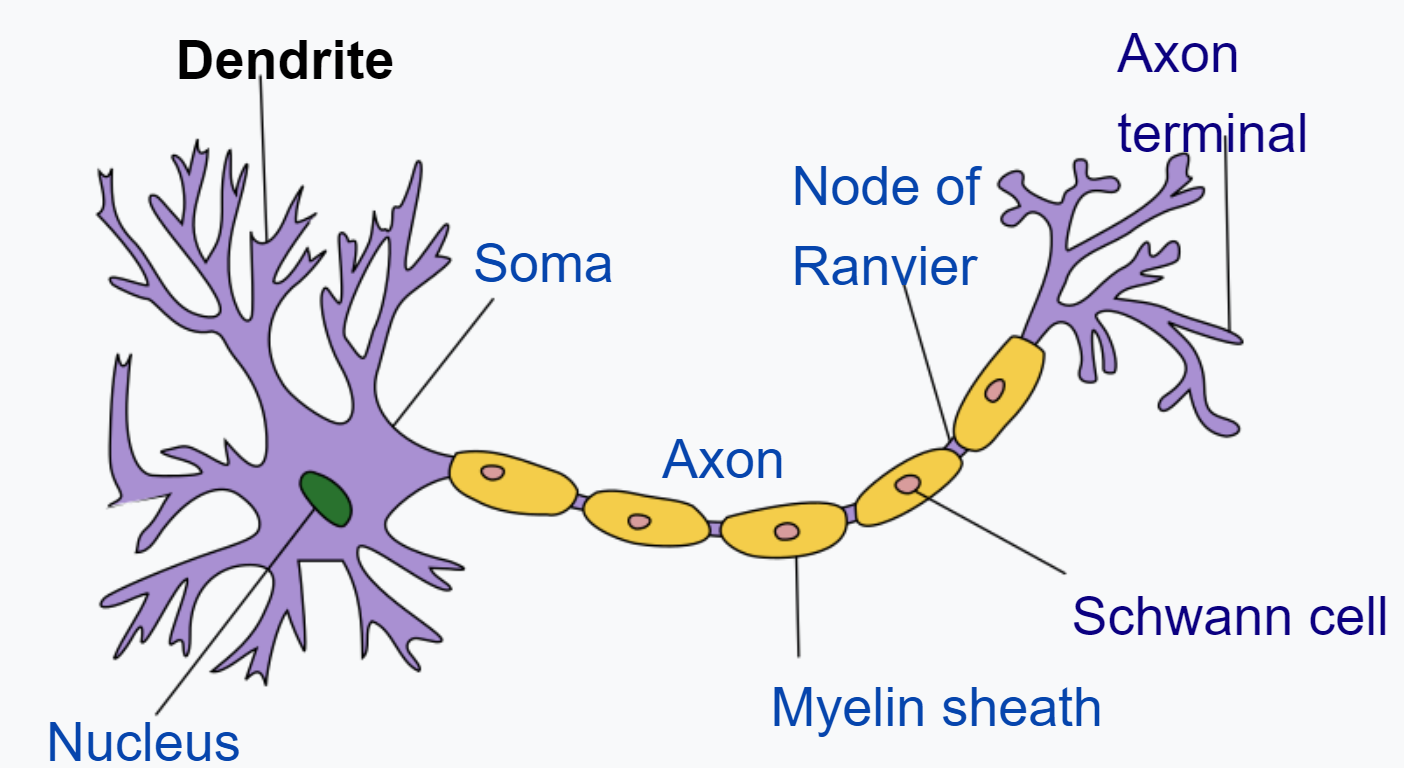
\includegraphics[width=2.8in]{./images/neuron.png}
        \caption{Neuron in the brain}
    \end{figure}
    
    \item Visually, a simple forward propagation looks like:
    \begin{figure}[H]
        \centering
        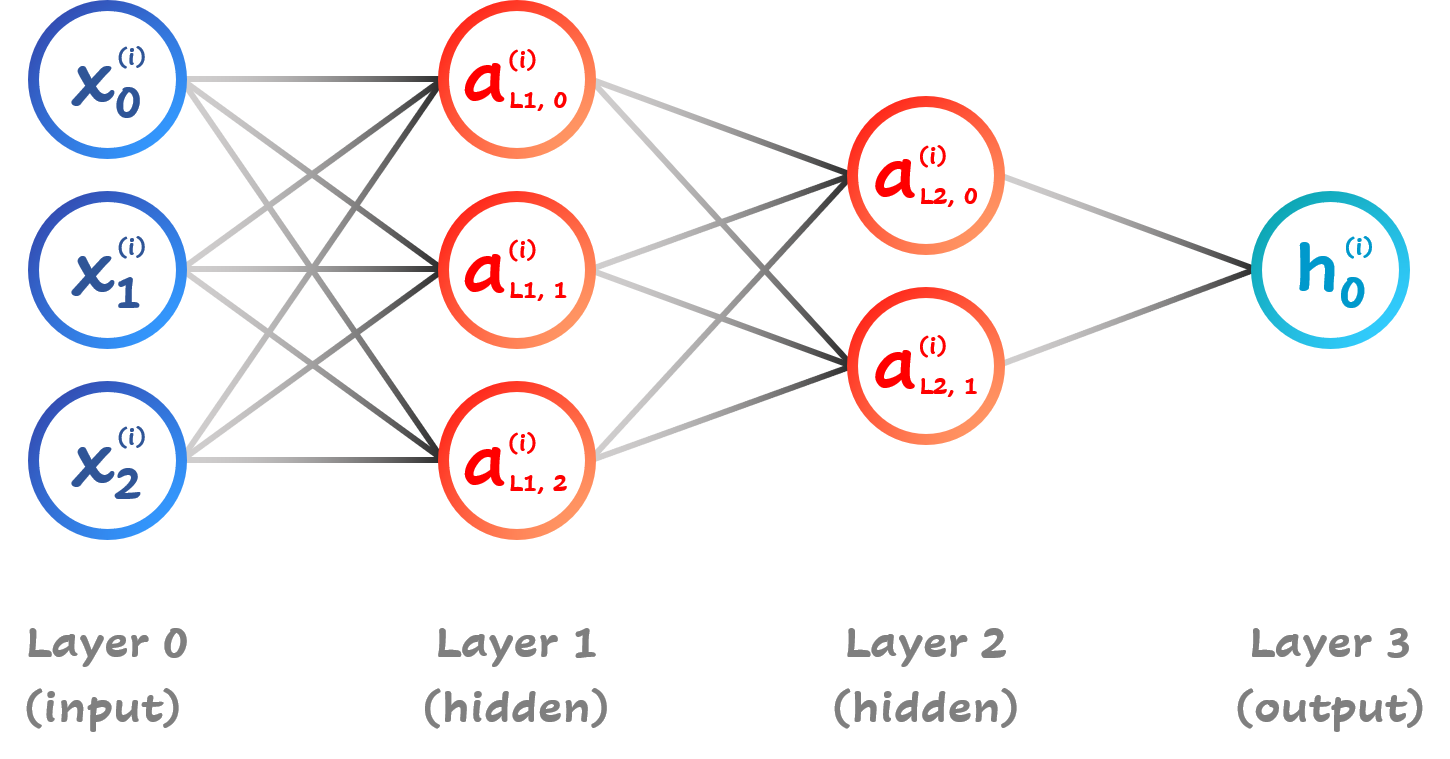
\includegraphics[width=3.8in]{./images/neuron_networks_architecture.png}
        \caption{Neural networks architecture}
    \end{figure}

    \begin{figure}[H]
        \centering
        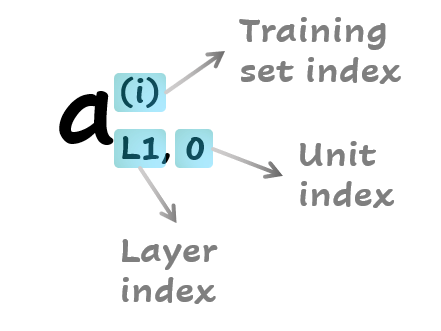
\includegraphics[width=2.1in]{./images/super_subscript.png}
        \caption{The convention of the superscript and subscript in neural networks}
    \end{figure}
    
    \item Neural networks can also do multiclass classification
    \begin{figure}[H]
        \centering
        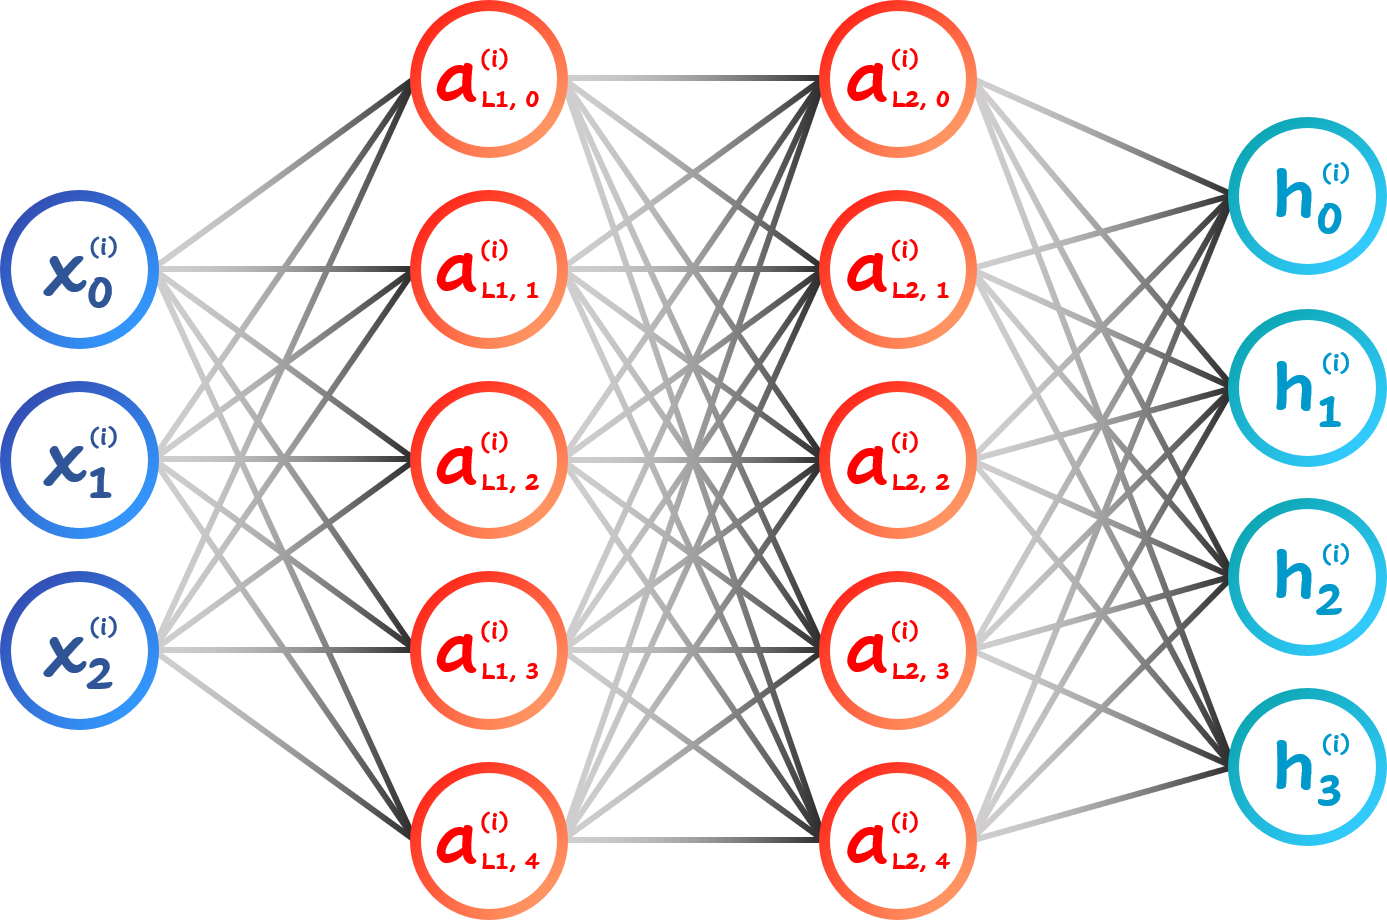
\includegraphics[width=3.8in]{./images/multiClassClassification.png}
        \caption{neural network for multi-class classification}
    \end{figure}

    \begin{equation}
        \mathbf{h} \approx \left\{ \begin{array}{l}

        \left[ \begin{matrix} 1 & 0 & 0 & 0 \end{matrix} \right]^T \text{, for pedestrian}\\
        \left[ \begin{matrix} 0 & 1 & 0 & 0 \end{matrix} \right]^T \text{, for car}\\
        \left[ \begin{matrix} 0 & 0 & 1 & 0 \end{matrix} \right]^T \text{, for motocycle}\\
        \left[ \begin{matrix} 0 & 0 & 0 & 1 \end{matrix} \right]^T \text{, for truck}\\

        \end{array}\right.
    \end{equation}

    \item In neural networks, the logistic function is sometimes called a \textbf{activation} function. In this situation, parameters are sometimes called \textbf{weights}.
    The values for each of the activation nodes is obtained as follows:
    \begin{equation}
        \begin{aligned}
            a_{L1,0} &= g(\theta_{L1, 00}x_0 + \theta_{L1, 01}x_1 + \theta_{L1, 02}x_2 + \theta_{L1, 03}x_3) &= g(z_{L1, 0})\\
            a_{L1,1} &= g(\theta_{L1, 10}x_0 + \theta_{L1, 11}x_1 + \theta_{L1, 12}x_2 + \theta_{L1, 13}x_3) &= g(z_{L1, 0})\\
            a_{L1,2} &= g(\theta_{L1, 20}x_0 + \theta_{L1, 21}x_1 + \theta_{L1, 22}x_2 + \theta_{L1, 23}x_3) &= g(z_{L1, 0})\\
        \end{aligned}
    \end{equation}

    Where $a_{Lj,i}$ means the activation of \textbf{unit} $i$ in layer $j$, and $\Theta_{Lj}$ means a mapping matrix of weights from layer $j-1$ to layer $j$.
    If there are $s_j$ units in layer $j$ and $s_{j-1}$ units in layer $j-1$, then.
    \begin{equation}
        \Theta_{Lj} =
        \left[
        \begin{matrix}
            \theta_{Lj, 00}     & \theta_{Lj, 01}     & \dots   & \theta_{Lj, 0{s_{j-1}}}     \\
            \theta_{Lj, 10}     & \theta_{Lj, 11}     & \dots   & \theta_{Lj, 1{s_{j-1}}}     \\
            \vdots              & \vdots              & \ddots  & \vdots                      \\
            \theta_{Lj, {s_j}0} & \theta_{Lj, {s_j}1} & \dots   & \theta_{Lj, {s_j}{s_{j-1}}} \\
        \end{matrix}
        \right]_{{(s_j+1)} \times {(s_{j-1}+1)}}
    \end{equation}
\end{itemize}

    
\section{Simplified Expressions}
\begin{itemize}
    \item The neural network looks too fancy. Let's try to make it simpler but more boring. The network could be expressed like:

    \begin{equation}
        \left[\begin{matrix} x^{(i)}_0 \\ x^{(i)}_1 \\ x^{(i)}_2 \end{matrix}\right]_{3 \times 1} \xRightarrow{[\Theta_{L1}]_{5 \times 3}}
        \left[\begin{matrix} a^{(i)}_{L1, 0} \\ a^{(i)}_{L1, 1} \\ a^{(i)}_{L1, 2} \\ a^{(i)}_{L1, 3} \\ a^{(i)}_{L1, 4} \end{matrix}\right]_{5 \times 1} \xRightarrow{[\Theta_{L2}]_{5 \times 5}}
        \left[\begin{matrix} a^{(i)}_{L2, 0} \\ a^{(i)}_{L2, 1} \\ a^{(i)}_{L2, 2} \\ a^{(i)}_{L2, 3} \\ a^{(i)}_{L2, 4} \end{matrix}\right]_{5 \times 1} \xRightarrow{[\Theta_{L3}]_{4 \times 5}}
        \left[\begin{matrix} h_0 \\ h_1 \\ h_2 \\ h_3 \end{matrix}\right]_{4 \times 1}
    \end{equation}

    \item Or in a vectorized form:
    \begin{equation}
        \mathbf{x}^{(i)} \xRightarrow{\Theta_{L1}}
        \mathbf{a}^{(i)}_{L1} \xRightarrow{\Theta_{L2}}
        \mathbf{a}^{(i)}_{L2} \xRightarrow{\Theta_{L3}}
        \mathbf{h}^{(i)}
    \end{equation}

    \item Actually, only three linear algebra equations are needed for this neural network
    \begin{equation}
        \begin{aligned}
            \mathbf{a}^{(i)}_{L1} &= g(\Theta_{L1} \times \mathbf{x}^{(i)})\\
            \mathbf{a}^{(i)}_{L2} &= g(\Theta_{L2} \times \mathbf{a}^{(i)}_{L1})\\
            \mathbf{h}^{(i)}      &= g(\Theta_{L3} \times \mathbf{a}^{(i)}_{L2})\\
        \end{aligned}
    \end{equation}
\end{itemize}

\section{Cost Function}
\begin{itemize}
    \item The cost function of a neural network with $m$ data sets, $K$ classifications and $L$ layers
    \begin{equation}
        J(\theta) = \frac{-1}{m}\sum_{i=1}^{m}\sum_{k=1}^{K}\left[ y^{(i)}_k \log\left(h^{(i)}_k\right) + \left(1 - y^{(i)}_k \right) \log\left(1 - h^{(i)}_k\right) \right] + \frac{\lambda}{2m}\sum_{l=1}^{L}||\Theta_{Ll}||_2^2
    \end{equation}
    Where $||\Theta_{Ll}||_2$ means \href{https://mathworld.wolfram.com/FrobeniusNorm.html}{Frobenius norm} of the matrix $\Theta_{Ll}$ 
\end{itemize}


\section{Backpropagation Algorithm}
\begin{itemize}
    \item Consider a simple neural network with only one data set
    \begin{figure}[H]
        \centering
        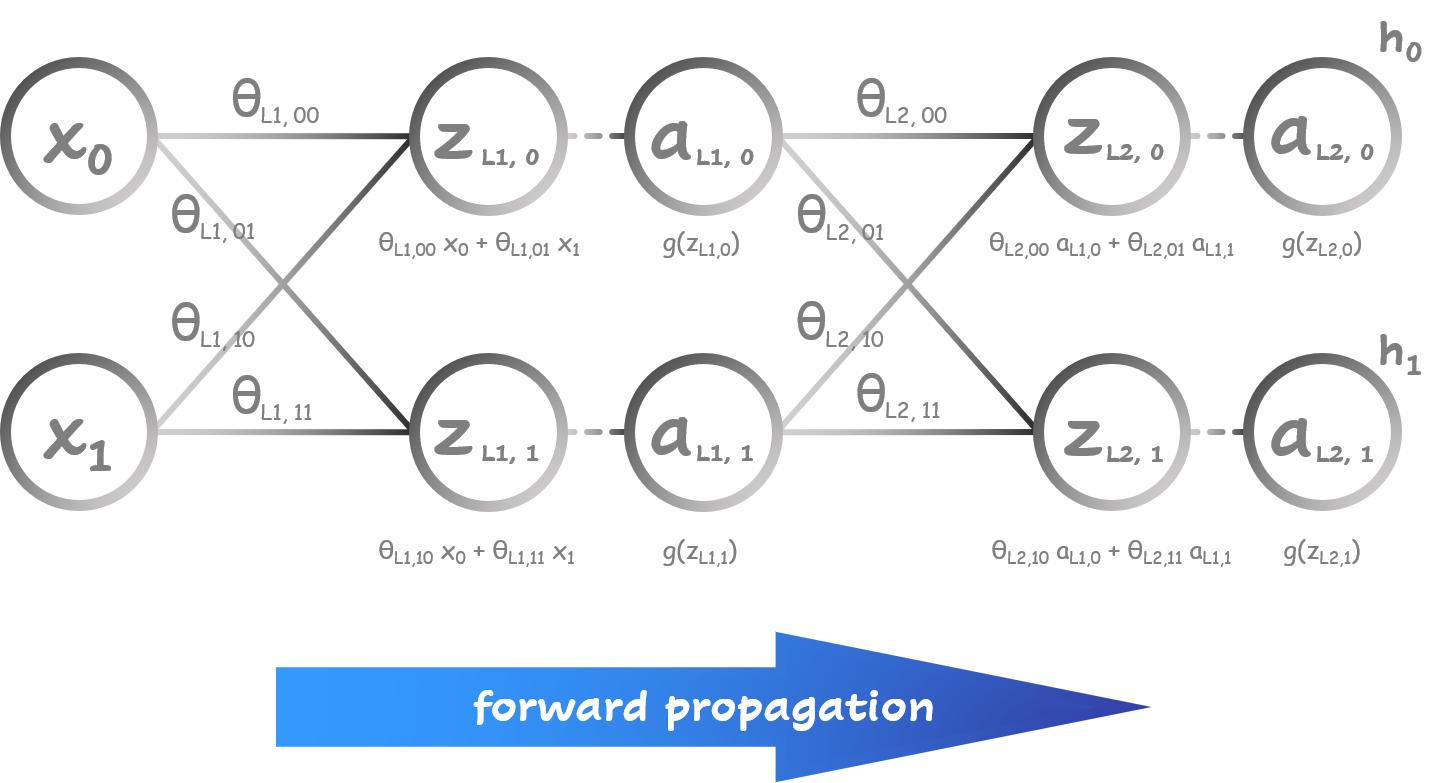
\includegraphics[width=4.8in]{./images/neural_network_forward.png}
        \caption{A simple neural network}
    \end{figure}
    
    The cost function would be
    \begin{equation}
        J(\theta) = \left[ 
                        y_0 \log\left(h_0\right) + \left(1 - y_0 \right) \log\left(1 - h_0\right) + 
                        y_1 \log\left(h_1\right) + \left(1 - y_1 \right) \log\left(1 - h_1\right) 
                    \right]
    \end{equation}

    And the gradient descent iteration would be:
    \begin{equation}
        \theta_{l, ij} \coloneqq \theta_{l, ij} - \alpha\frac{\partial J(\theta)}{\partial \theta_{l, ij}} 
    \end{equation}
    
    To compute the gradient descent for $\theta_{l, ij}$, it's needed to find out the regulation of $\frac{\partial J}{\partial \theta_{l,ij}}$.
    First, try to do the partial derivatives at the second layer.
    
    \begin{equation}
        \frac{\partial J}{\partial \theta_{L2,00}} = \frac{\partial J}{\partial a_{L2,0}}\frac{\partial a_{L2,0}}{\partial z_{L2,0}}\frac{\partial z_{L2,0}}{\partial \theta_{L2,00}} = \frac{\partial J}{\partial a_{L2,0}} g'(z_{L2,0}) a_{L1,0}
    \end{equation}
    \begin{equation}
        \frac{\partial J}{\partial \theta_{L2,01}} = \frac{\partial J}{\partial a_{L2,0}}\frac{\partial a_{L2,0}}{\partial z_{L2,0}}\frac{\partial z_{L2,0}}{\partial \theta_{L2,01}} = \frac{\partial J}{\partial a_{L2,0}} g'(z_{L2,0}) a_{L1,1}
    \end{equation}
    \begin{equation}
        \frac{\partial J}{\partial \theta_{L2,10}} = \frac{\partial J}{\partial a_{L2,1}}\frac{\partial a_{L2,1}}{\partial z_{L2,1}}\frac{\partial z_{L2,1}}{\partial \theta_{L2,10}} = \frac{\partial J}{\partial a_{L2,1}} g'(z_{L2,1}) a_{L1,0}
    \end{equation}
    \begin{equation}
        \frac{\partial J}{\partial \theta_{L2,11}} = \frac{\partial J}{\partial a_{L2,1}}\frac{\partial a_{L2,1}}{\partial z_{L2,1}}\frac{\partial z_{L2,1}}{\partial \theta_{L2,11}} = \frac{\partial J}{\partial a_{L2,1}} g'(z_{L2,1}) a_{L1,1}
    \end{equation}
    
    Then, try to do the partial derivatives at the first layer.
    \begin{equation}\label{eqn:partialDerivative}
        \begin{aligned}
            \frac{\partial J}{\partial \theta_{L1,00}} &= \left({ \frac{\partial J}{\partial a_{L2,0}}\frac{\partial a_{L2,0}}{\partial z_{L2,0}}\frac{\partial z_{L2,0}}{\partial a_{L1,0}} + \frac{\partial J}{\partial a_{L2,1}}\frac{\partial a_{L2,1}}{\partial z_{L2,1}}\frac{\partial z_{L2,1}}{\partial a_{L1,0}} }\right) \frac{\partial a_{L1,0}}{\partial z_{L1,0}}\frac{\partial z_{L1,0}}{\partial \theta_{L1,00}}\\
                                                        &= \left({ \frac{\partial J}{\partial a_{L2,0}} g'(z_{L2,0}) \theta_{L2,00} + \frac{\partial J}{\partial a_{L2,1}} g'(z_{L2,1}) \theta_{L2,10}} \right) g'(z_{L1,0}) x_0 \\
                                                        &= \frac{\partial J}{\partial a_{L1,0}} g'(z_{L1,0}) x_0 \\
        \end{aligned}
    \end{equation}
    
    So the others would be like
    \begin{equation}
        \frac{\partial J}{\partial \theta_{L1,01}} = \frac{\partial J}{\partial a_{L1,0}} g'(z_{L1,0}) x_1
    \end{equation}
    \begin{equation}
        \frac{\partial J}{\partial \theta_{L1,10}} = \frac{\partial J}{\partial a_{L1,1}} g'(z_{L1,1}) x_0
    \end{equation}
    \begin{equation}
        \frac{\partial J}{\partial \theta_{L1,11}} = \frac{\partial J}{\partial a_{L1,1}} g'(z_{L1,1}) x_1
    \end{equation}
    
    It can be seen that $\frac{\partial{J}}{\partial{a_{l,i}}}$ are necessary for $\frac{\partial{J}}{\partial{\theta_{l,ij}}}$.
    However, if using a forward propagation to do the gradient descent process,
    it would be unavailable for $\frac{\partial{J}}{\partial{a_{l,i}}}$ at a previous layer because of the dependency in a neural network.
    To solve this inconvenience, backpropagation should be adopted.
    
    That is to say the training processes of a neural network containing 
    one forward process to get the values of each activations ($a_{l,i}$) and 
    one backpropagation process to get the values of derivatives corresponded to each activations ($\frac{\partial{J}}{\partial{a_{L,i}}}$).
    Then the values derived from the backpropagation are necessary for the gradient descent process.
    
    Observe equation \ref{eqn:partialDerivative}, there is a regulation of $\frac{\partial{J}}{\partial{a_{l,i}}}$ can be found. 
    The regulation can be seen as actions of the backpropagation process in Figure \ref{fig:backpropagation}.
    
    \begin{figure}[H] \label{fig:backpropagation}
        \centering
        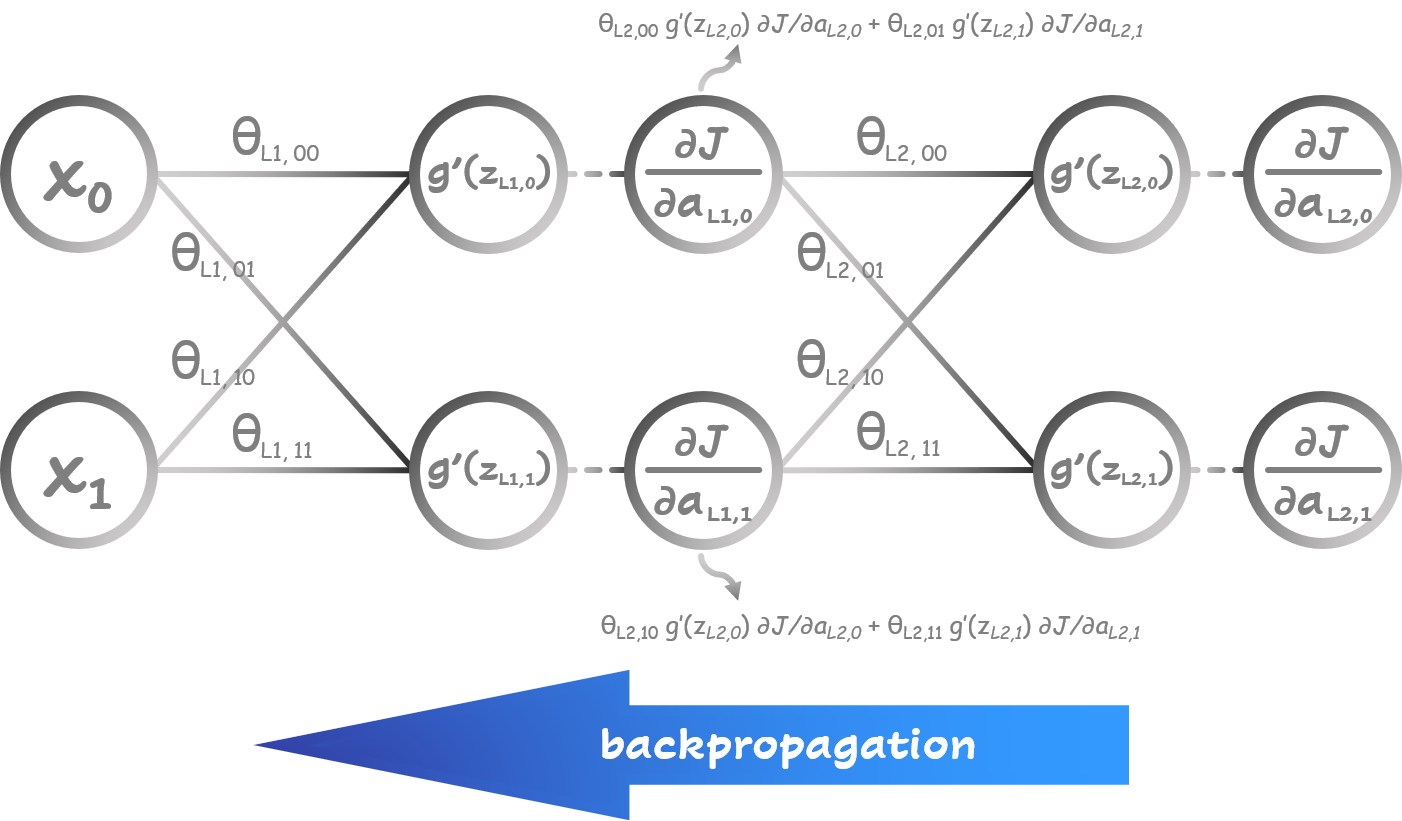
\includegraphics[width=4.8in]{./images/neural_network_back.png}
        \caption{The backpropagation in a neural network}
    \end{figure}
    
    Once the backpropagation process was completed, the partial derivatives of each weight ($\frac{\partial J}{\partial \theta_{l,ij}}$) 
    can computed which is shown as figure \ref{fig:gradientDescentNN} and equation \ref{eqn:gradientDescentNN}
    
    \begin{figure}[H] \label{fig:gradientDescentNN}
        \centering
        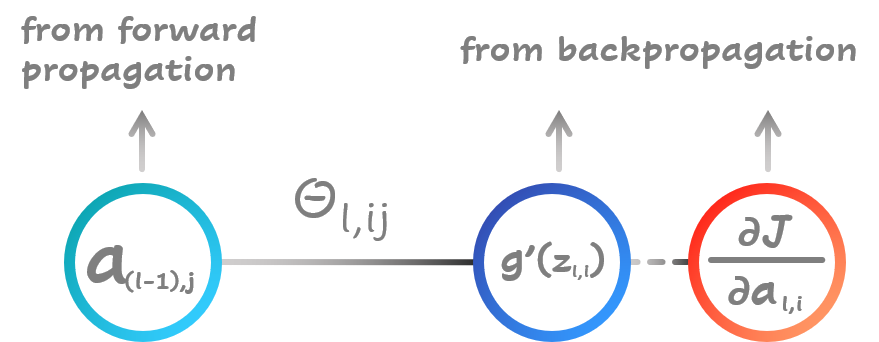
\includegraphics[width=3.6in]{./images/gradient_descent_neural_network.png}
        \caption{The backpropagation in a neural network}
    \end{figure}
    
    \begin{equation} \label{eqn:gradientDescentNN}
        \frac{\partial J}{\partial \theta_{l,ij}} = \color{RedOrange} \frac{\partial J}{\partial a_{l,i}} \color{blue} g'(z_{l,i}) \color{cyan} a_{(l-1),j} \color{black}
    \end{equation}
\end{itemize}
    
    
\section{Non-linear Classification Example}
\begin{itemize}
    \item Logical functions in figure \ref{fig:logicGates} would be examples to show how neural networks really work.
    \begin{figure}[H]\label{fig:logicGates}
        \centering
        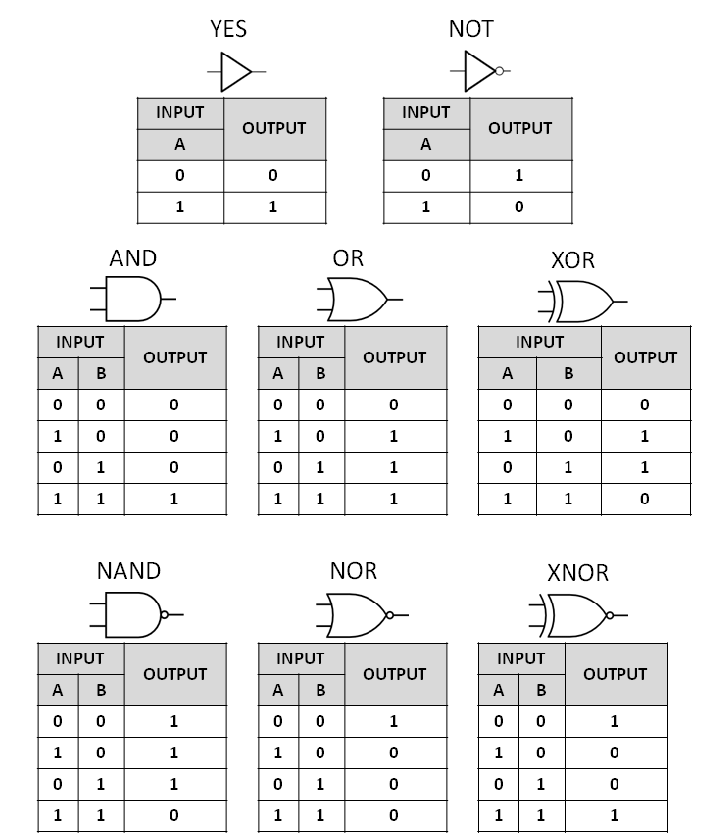
\includegraphics[width=3.6in]{./images/logicGates.png}
        \caption{The common Boolean logic gates with symbols and truth tables}
    \end{figure}
    
    % \item First, remind that sigmoid function looks like figure \ref{fig:RemindSigmoid}.
    \begin{figure}[H]\label{fig:RemindSigmoid}
        \centering
        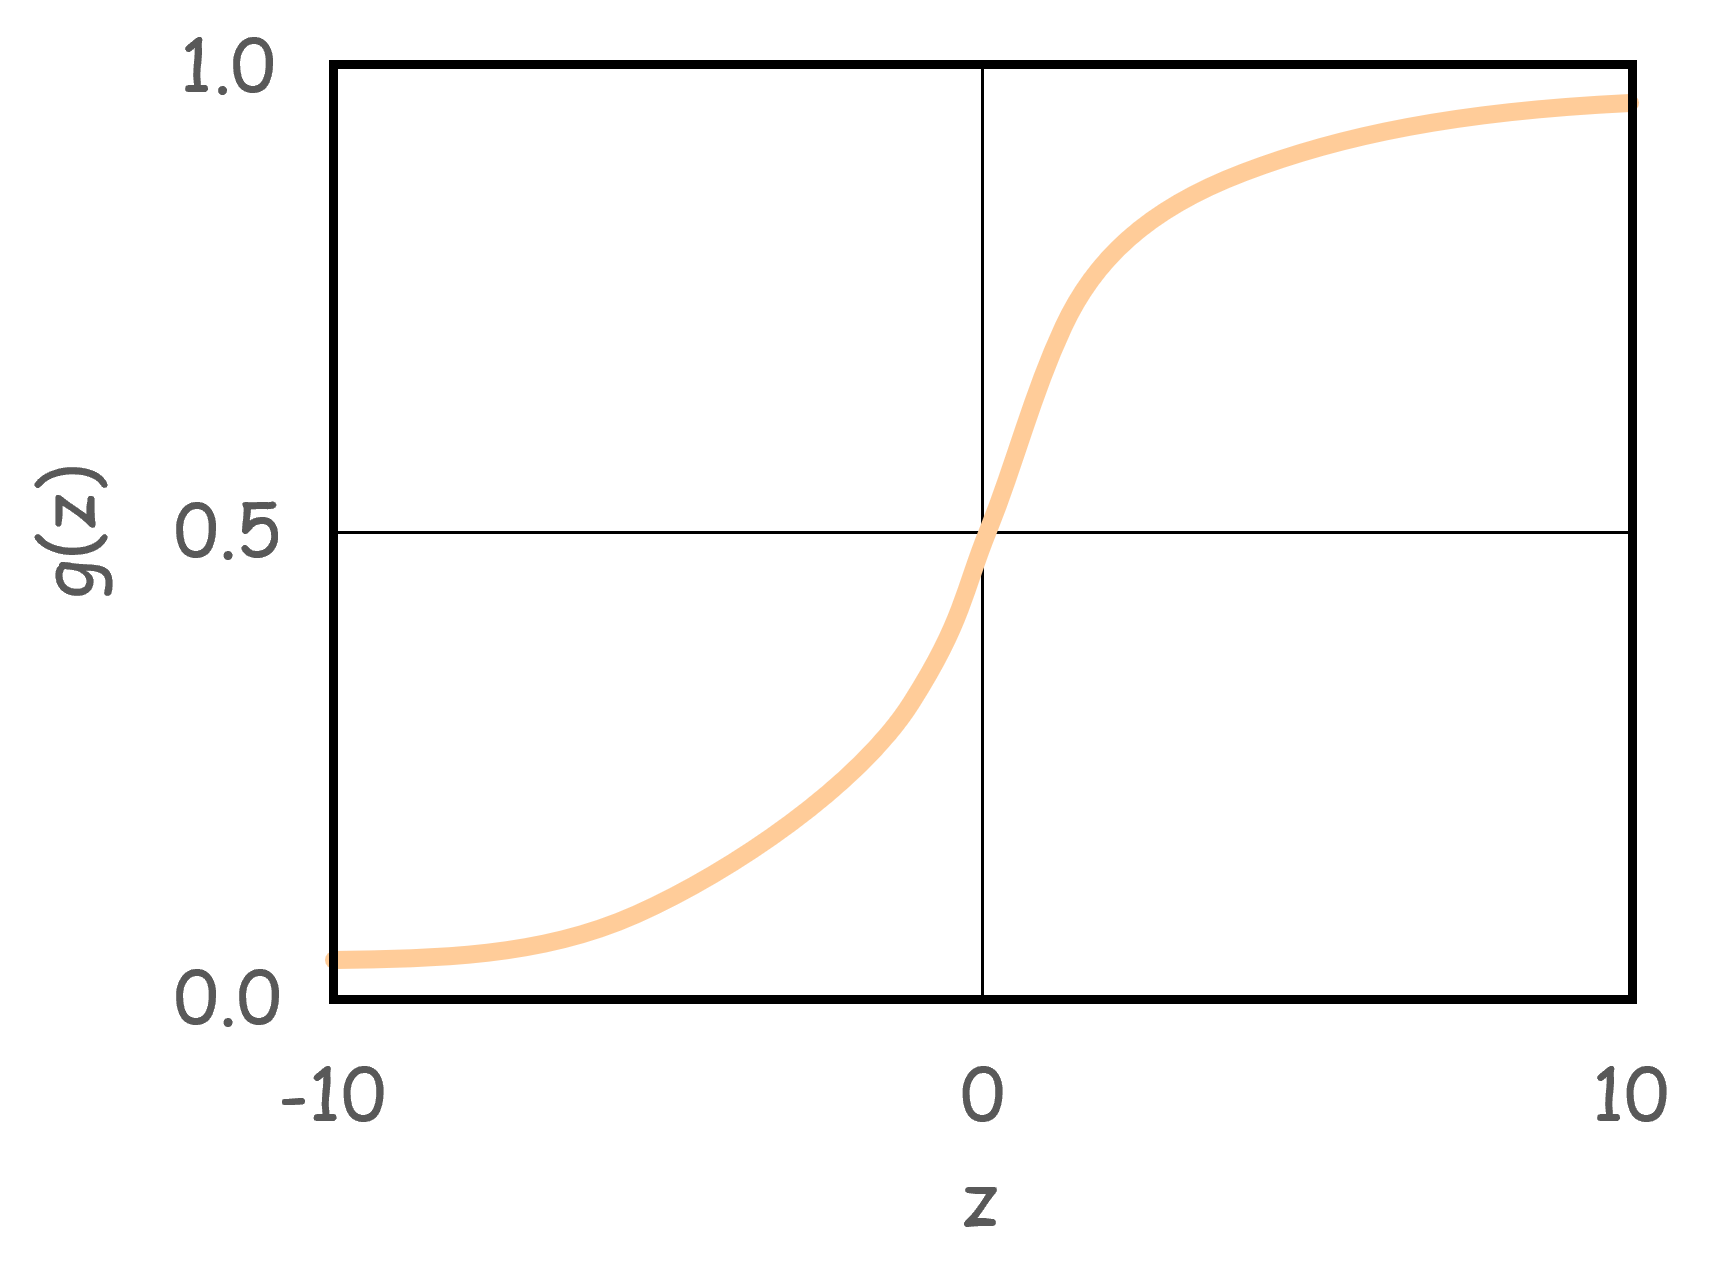
\includegraphics[width=2.8in]{./images/sigmoid.png}
        \caption{Logistic function}
    \end{figure}
    
    \begin{figure}[H]
        \centering
        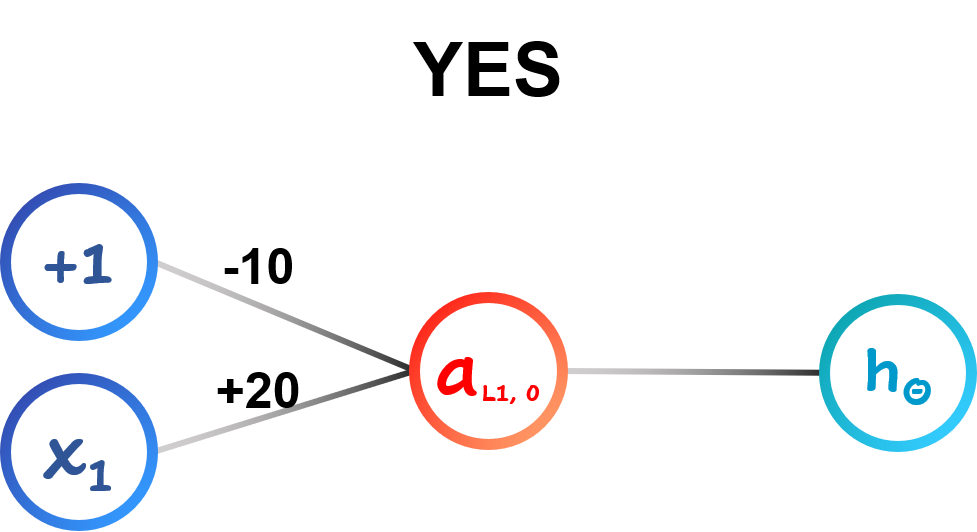
\includegraphics[width=2.4in]{./images/logicGate_YES.png}
        \caption{neural network of logical function YES}
    \end{figure}

    \begin{table}[H]
        \renewcommand\arraystretch{1.5}
        \caption{YES calculation}
        \centering
        \begin{tabular}{ccc}
            \hline\hline %%%%%%%%%%%%%%%%%%%%%%%%%%%%%%%%%%%%%%%%%%%%%%%%%%%%%%%%%%%%%%%%%%%%%%%%%%%%
            Inputs                                                 & Activations        & Outputs    \\ 
            $\begin{array}{ccc} x_0 & x_1 \end{array}$             & $a^{(1)}_0$        & $h$        \\ 
            \hline %%%%%%%%%%%%%%%%%%%%%%%%%%%%%%%%%%%%%%%%%%%%%%%%%%%%%%%%%%%%%%%%%%%%%%%%%%%%%%%%%%
            $\left[{\begin{array}{ccc} 1 & 0 \end{array}}\right]$  & $g(-10) \approx 0$ & $0$        \\
            $\left[{\begin{array}{ccc} 1 & 1 \end{array}}\right]$  & $g(+10) \approx 1$ & $1$        \\[1ex]
            \hline\hline %%%%%%%%%%%%%%%%%%%%%%%%%%%%%%%%%%%%%%%%%%%%%%%%%%%%%%%%%%%%%%%%%%%%%%%%%%%%
        \end{tabular}
    \end{table}
    
    \begin{figure}[H]
        \centering
        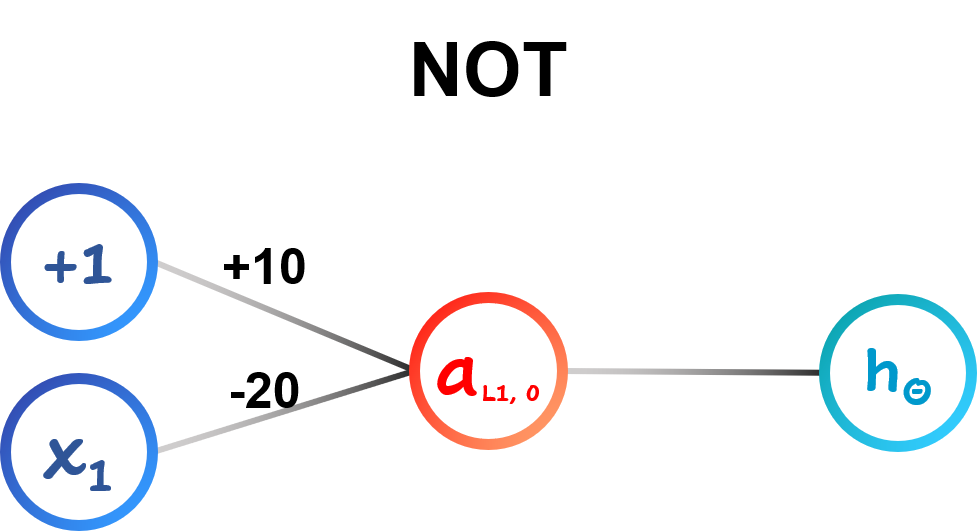
\includegraphics[width=2.4in]{./images/logicGate_NOT.png}
        \caption{neural network of logical function NOT}
    \end{figure}

    \begin{table}[H]
        \renewcommand\arraystretch{1.5}
        \caption{NOT calculation}
        \centering
        \begin{tabular}{ccc}
            \hline\hline %%%%%%%%%%%%%%%%%%%%%%%%%%%%%%%%%%%%%%%%%%%%%%%%%%%%%%%%%%%%%%%%%%%%%%%%%%%%
            Inputs                                                 & Activations        & Outputs    \\ 
            $\begin{array}{ccc} x_0 & x_1 \end{array}$             & $a^{(1)}_0$        & $h$        \\ 
            \hline %%%%%%%%%%%%%%%%%%%%%%%%%%%%%%%%%%%%%%%%%%%%%%%%%%%%%%%%%%%%%%%%%%%%%%%%%%%%%%%%%%
            $\left[{\begin{array}{ccc} 1 & 0 \end{array}}\right]$  & $g(+10) \approx 1$ & $1$        \\
            $\left[{\begin{array}{ccc} 1 & 1 \end{array}}\right]$  & $g(-10) \approx 0$ & $0$        \\[1ex]
            \hline\hline %%%%%%%%%%%%%%%%%%%%%%%%%%%%%%%%%%%%%%%%%%%%%%%%%%%%%%%%%%%%%%%%%%%%%%%%%%%%
        \end{tabular}
    \end{table}
    
    \begin{figure}[H]
        \centering
        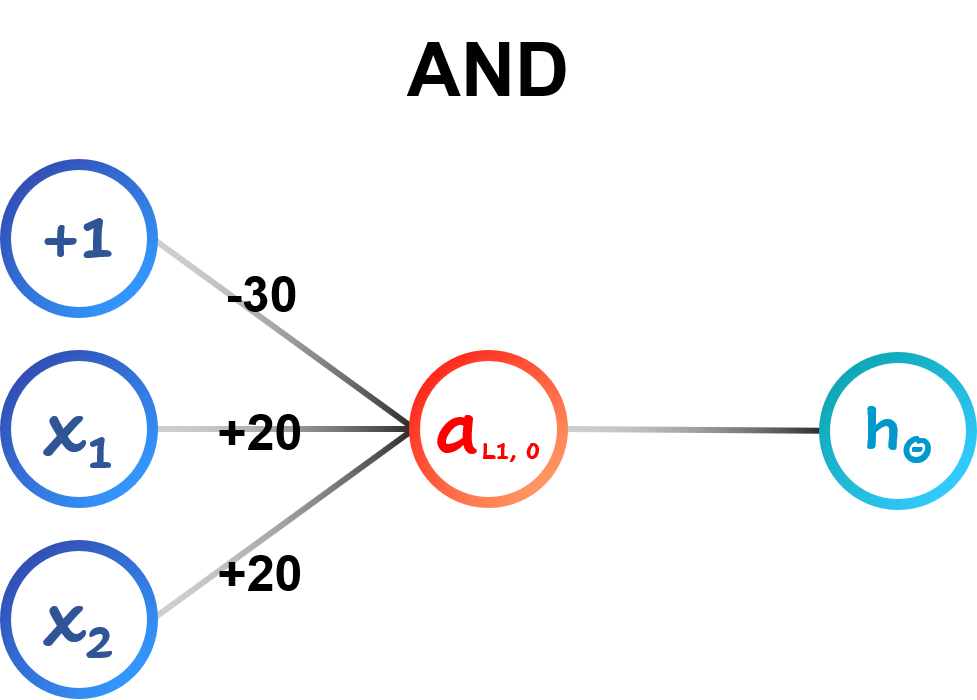
\includegraphics[width=2.4in]{./images/logicGate_AND.png}
        \caption{neural network of logical function AND}
    \end{figure}

    \begin{table}[H]
        \renewcommand\arraystretch{1.5}
        \caption{AND calculation}
        \centering
        \begin{tabular}{ccc}
            \hline\hline %%%%%%%%%%%%%%%%%%%%%%%%%%%%%%%%%%%%%%%%%%%%%%%%%%%%%%%%%%%%%%%%%%%%%%%%%%%%%%%%%%
            Inputs                                                     & Activations        & Outputs    \\ 
            $\begin{array}{ccc} x_0 & x_1 & x_2 \end{array}$           & $a^{(1)}_0$        & $h$        \\ 
            \hline %%%%%%%%%%%%%%%%%%%%%%%%%%%%%%%%%%%%%%%%%%%%%%%%%%%%%%%%%%%%%%%%%%%%%%%%%%%%%%%%%%%%%%%%
            $\left[{\begin{array}{ccc} 1 & 0 & 0 \end{array}}\right]$  & $g(-30) \approx 0$ & $0$        \\ 
            $\left[{\begin{array}{ccc} 1 & 0 & 1 \end{array}}\right]$  & $g(-10) \approx 0$ & $0$        \\
            $\left[{\begin{array}{ccc} 1 & 1 & 0 \end{array}}\right]$  & $g(-10) \approx 0$ & $0$        \\
            $\left[{\begin{array}{ccc} 1 & 1 & 1 \end{array}}\right]$  & $g(+10) \approx 1$ & $1$        \\[1ex]
            \hline\hline %%%%%%%%%%%%%%%%%%%%%%%%%%%%%%%%%%%%%%%%%%%%%%%%%%%%%%%%%%%%%%%%%%%%%%%%%%%%%%%%%%
        \end{tabular}
    \end{table}

    \begin{figure}[H]
        \centering
        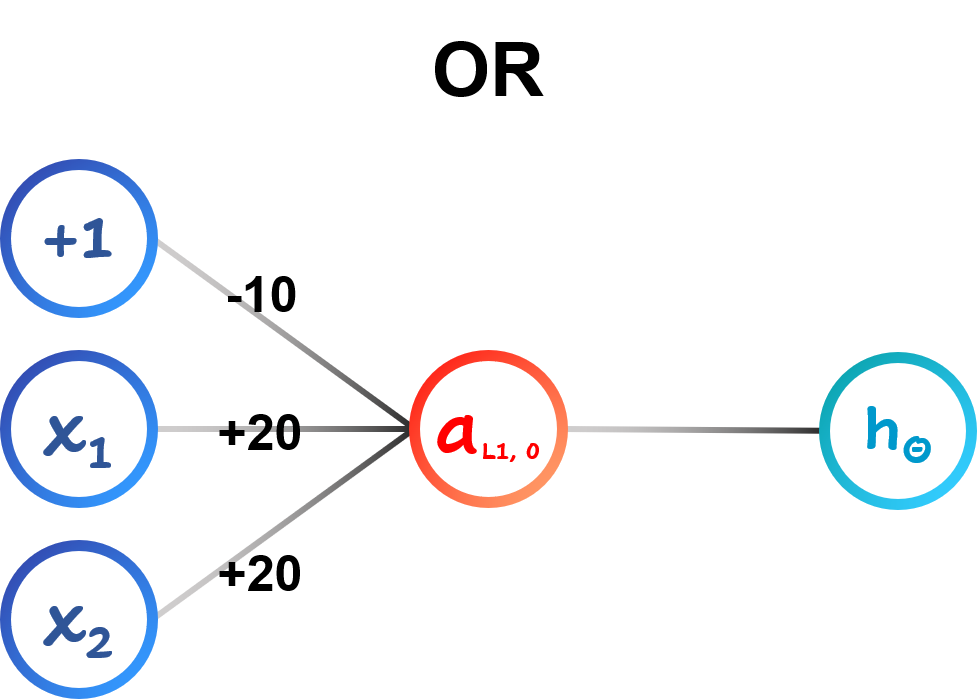
\includegraphics[width=2.4in]{./images/logicGate_OR.png}
        \caption{neural network of logical function OR}
    \end{figure}

    \begin{table}[H]
        \renewcommand\arraystretch{1.5}
        \caption{OR calculation}
        \centering
        \begin{tabular}{ccc}
            \hline\hline %%%%%%%%%%%%%%%%%%%%%%%%%%%%%%%%%%%%%%%%%%%%%%%%%%%%%%%%%%%%%%%%%%%%%%%%%%%%%%%%%%
            Inputs                                                     & Activations        & Outputs    \\ 
            $\begin{array}{ccc} x_0 & x_1 & x_2 \end{array}$           & $a^{(1)}_0$        & $h$        \\ 
            \hline %%%%%%%%%%%%%%%%%%%%%%%%%%%%%%%%%%%%%%%%%%%%%%%%%%%%%%%%%%%%%%%%%%%%%%%%%%%%%%%%%%%%%%%%
            $\left[{\begin{array}{ccc} 1 & 0 & 0 \end{array}}\right]$  & $g(-10) \approx 0$ & $0$        \\ 
            $\left[{\begin{array}{ccc} 1 & 0 & 1 \end{array}}\right]$  & $g(+10) \approx 1$ & $1$        \\
            $\left[{\begin{array}{ccc} 1 & 1 & 0 \end{array}}\right]$  & $g(+10) \approx 1$ & $1$        \\
            $\left[{\begin{array}{ccc} 1 & 1 & 1 \end{array}}\right]$  & $g(+30) \approx 1$ & $1$        \\[1ex]
            \hline\hline %%%%%%%%%%%%%%%%%%%%%%%%%%%%%%%%%%%%%%%%%%%%%%%%%%%%%%%%%%%%%%%%%%%%%%%%%%%%%%%%%%
        \end{tabular}
    \end{table}
    
    \begin{figure}[H]
        \centering
        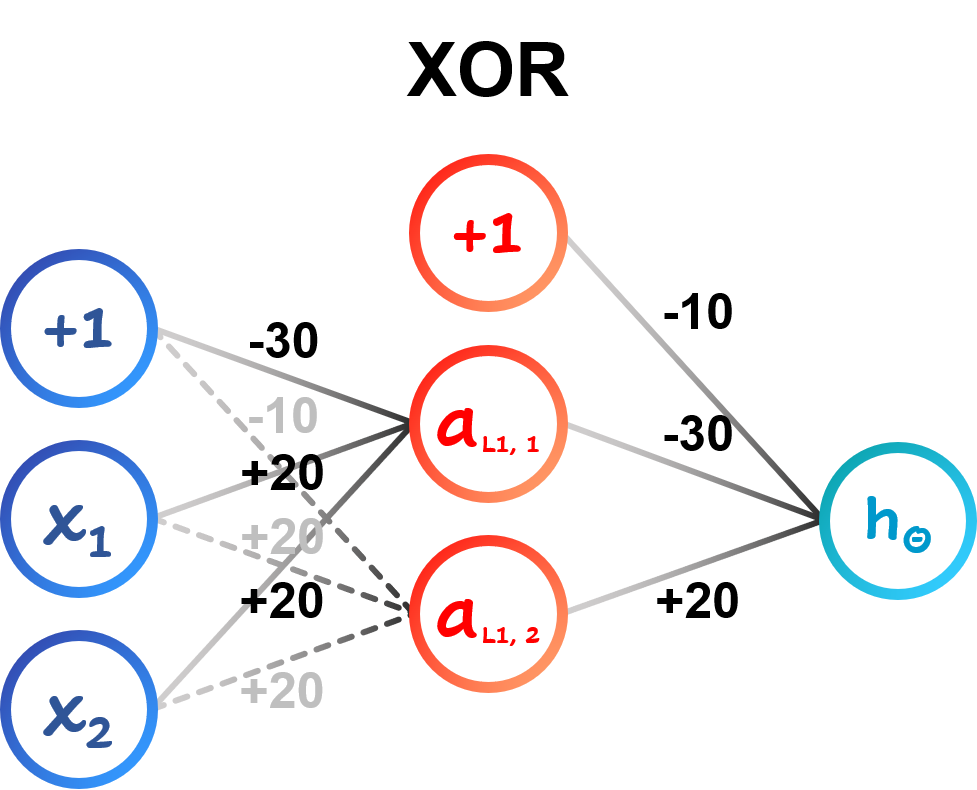
\includegraphics[width=2.4in]{./images/logicGate_XOR.png}
        \caption{neural network of logical function XOR}
    \end{figure}
    
    \begin{table}[H]
        \renewcommand\arraystretch{1.5}
        \caption{XOR calculation}
        \centering
        \begin{tabular}{ccc}
            \hline\hline %%%%%%%%%%%%%%%%%%%%%%%%%%%%%%%%%%%%%%%%%%%%%%%%%%%%%%%%%%%%%%%%%%%%%%%%%%%%%%%%%%%%%%%%%%%%%%%%%%%%%%%%%%%%%%%%%%%%%%%%%%%%%%%%%%%%%%%%%%%%%%%%%%%%%%%%%%%%%%%%%%%%%%%%%%%%%%%%%%%%%%%%%%%%%%%%%%%%%%%%%%%
            Inputs                                                     & Activations                                                                                                                         & Outputs            \\ 
            $\begin{array}{ccc} x_0 & x_1 & x_2 \end{array}$           & $\begin{array}{ccc} a^{(1)}_0 & a^{(1)}_1 & a^{(1)}_2 \end{array}$                                                                  & $h$                \\ 
            \hline %%%%%%%%%%%%%%%%%%%%%%%%%%%%%%%%%%%%%%%%%%%%%%%%%%%%%%%%%%%%%%%%%%%%%%%%%%%%%%%%%%%%%%%%%%%%%%%%%%%%%%%%%%%%%%%%%%%%%%%%%%%%%%%%%%%%%%%%%%%%%%%%%%%%%%%%%%%%%%%%%%%%%%%%%%%%%%%%%%%%%%%%%%%%%%%%%%%%%%%%%%%%%%%%%
            $\left[{\begin{array}{ccc} 1 & 0 & 0 \end{array}}\right]$  & $\left[{\begin{array}{ccc} 1 & g(-30) & g(-10) \end{array}}\right] \approx \left[{\begin{array}{ccc} 1 & 0 & 0 \end{array}}\right]$ & $g(-10) \approx 0$ \\ 
            $\left[{\begin{array}{ccc} 1 & 0 & 1 \end{array}}\right]$  & $\left[{\begin{array}{ccc} 1 & g(-10) & g(+10) \end{array}}\right] \approx \left[{\begin{array}{ccc} 1 & 0 & 1 \end{array}}\right]$ & $g(+10) \approx 1$ \\
            $\left[{\begin{array}{ccc} 1 & 1 & 0 \end{array}}\right]$  & $\left[{\begin{array}{ccc} 1 & g(-10) & g(+10) \end{array}}\right] \approx \left[{\begin{array}{ccc} 1 & 0 & 1 \end{array}}\right]$ & $g(+10) \approx 1$ \\
            $\left[{\begin{array}{ccc} 1 & 1 & 1 \end{array}}\right]$  & $\left[{\begin{array}{ccc} 1 & g(+10) & g(+30) \end{array}}\right] \approx \left[{\begin{array}{ccc} 1 & 1 & 1 \end{array}}\right]$ & $g(-10) \approx 0$ \\[1ex]
            \hline\hline %%%%%%%%%%%%%%%%%%%%%%%%%%%%%%%%%%%%%%%%%%%%%%%%%%%%%%%%%%%%%%%%%%%%%%%%%%%%%%%%%%%%%%%%%%%%%%%%%%%%%%%%%%%%%%%%%%%%%%%%%%%%%%%%%%%%%%%%%%%%%%%%%%%%%%%%%%%%%%%%%%%%%%%%%%%%%%%%%%%%%%%%%%%%%%%%%%%%%%%%%%%
        \end{tabular}
    \end{table}

    \begin{figure}[H]
        \centering
        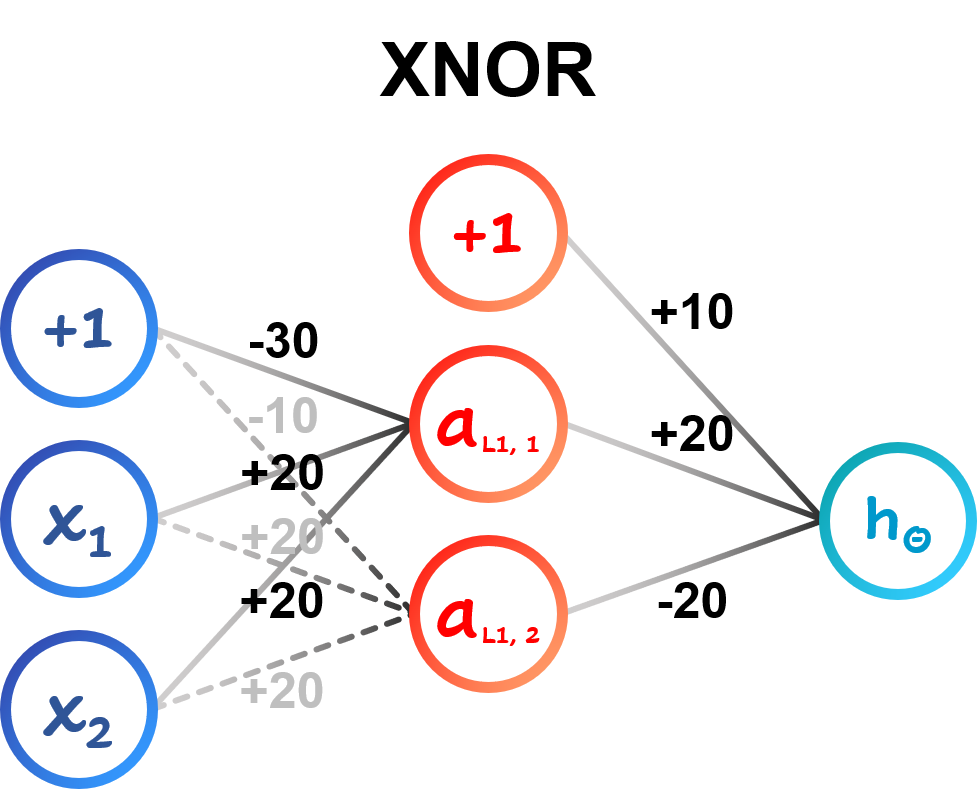
\includegraphics[width=2.4in]{./images/logicGate_XNOR.png}
        \caption{neural network of logical function XNOR}
    \end{figure}
    
    \begin{table}[H]
        \renewcommand\arraystretch{1.5}
        \caption{XNOR calculation}
        \centering
        \begin{tabular}{ccc}
            \hline\hline %%%%%%%%%%%%%%%%%%%%%%%%%%%%%%%%%%%%%%%%%%%%%%%%%%%%%%%%%%%%%%%%%%%%%%%%%%%%%%%%%%%%%%%%%%%%%%%%%%%%%%%%%%%%%%%%%%%%%%%%%%%%%%%%%%%%%%%%%%%%%%%%%%%%%%%%%%%%%%%%%%%%%%%%%%%%%%%%%%%%%%%%%%%%%%%%%%%%%%%%%%%
            Inputs                                                     & Activations                                                                                                                         & Outputs            \\ 
            $\begin{array}{ccc} x_0 & x_1 & x_2 \end{array}$           & $\begin{array}{ccc} a^{(1)}_0 & a^{(1)}_1 & a^{(1)}_2 \end{array}$                                                                  & $h$                \\ 
            \hline %%%%%%%%%%%%%%%%%%%%%%%%%%%%%%%%%%%%%%%%%%%%%%%%%%%%%%%%%%%%%%%%%%%%%%%%%%%%%%%%%%%%%%%%%%%%%%%%%%%%%%%%%%%%%%%%%%%%%%%%%%%%%%%%%%%%%%%%%%%%%%%%%%%%%%%%%%%%%%%%%%%%%%%%%%%%%%%%%%%%%%%%%%%%%%%%%%%%%%%%%%%%%%%%%
            $\left[{\begin{array}{ccc} 1 & 0 & 0 \end{array}}\right]$  & $\left[{\begin{array}{ccc} 1 & g(-30) & g(-10) \end{array}}\right] \approx \left[{\begin{array}{ccc} 1 & 0 & 0 \end{array}}\right]$ & $g(+10) \approx 1$ \\ 
            $\left[{\begin{array}{ccc} 1 & 0 & 1 \end{array}}\right]$  & $\left[{\begin{array}{ccc} 1 & g(-10) & g(+10) \end{array}}\right] \approx \left[{\begin{array}{ccc} 1 & 0 & 1 \end{array}}\right]$ & $g(-10) \approx 0$ \\
            $\left[{\begin{array}{ccc} 1 & 1 & 0 \end{array}}\right]$  & $\left[{\begin{array}{ccc} 1 & g(-10) & g(+10) \end{array}}\right] \approx \left[{\begin{array}{ccc} 1 & 0 & 1 \end{array}}\right]$ & $g(-10) \approx 0$ \\
            $\left[{\begin{array}{ccc} 1 & 1 & 1 \end{array}}\right]$  & $\left[{\begin{array}{ccc} 1 & g(+10) & g(+30) \end{array}}\right] \approx \left[{\begin{array}{ccc} 1 & 1 & 1 \end{array}}\right]$ & $g(+10) \approx 1$ \\[1ex]
            \hline\hline %%%%%%%%%%%%%%%%%%%%%%%%%%%%%%%%%%%%%%%%%%%%%%%%%%%%%%%%%%%%%%%%%%%%%%%%%%%%%%%%%%%%%%%%%%%%%%%%%%%%%%%%%%%%%%%%%%%%%%%%%%%%%%%%%%%%%%%%%%%%%%%%%%%%%%%%%%%%%%%%%%%%%%%%%%%%%%%%%%%%%%%%%%%%%%%%%%%%%%%%%%%
        \end{tabular}
    \end{table}    
\end{itemize}
        
    \chapter{Machine Learning Diagnostic}


\section{Splitting dataset}
\begin{itemize}
    \item To implement a diagonostic test, data sets can be divided into three parts: \textbf{training set} 60\%, \textbf{cross validation set} 20\% and \textbf{test set} 20\%.
    
    \begin{itemize}
        \item \textbf{training set}: to train the different candidate models during the learning process
        \item \textbf{validation set}: to compare performances of these models and decide which one to take, that is to tune the hyperparameters
        \item \textbf{test set}: only to assess the performance such as accuracy, sensitivity, specificity, F-measure, and so on
    \end{itemize}

    \item The cost functions of each sets would be $J_{\text{train}}$, $J_{\text{cv}}$, $J_{\text{test}}$

\end{itemize}


\section{Model selection}
\begin{itemize}
    \item Diagnose degree of polynomial
    \begin{figure}[H]
        \centering
        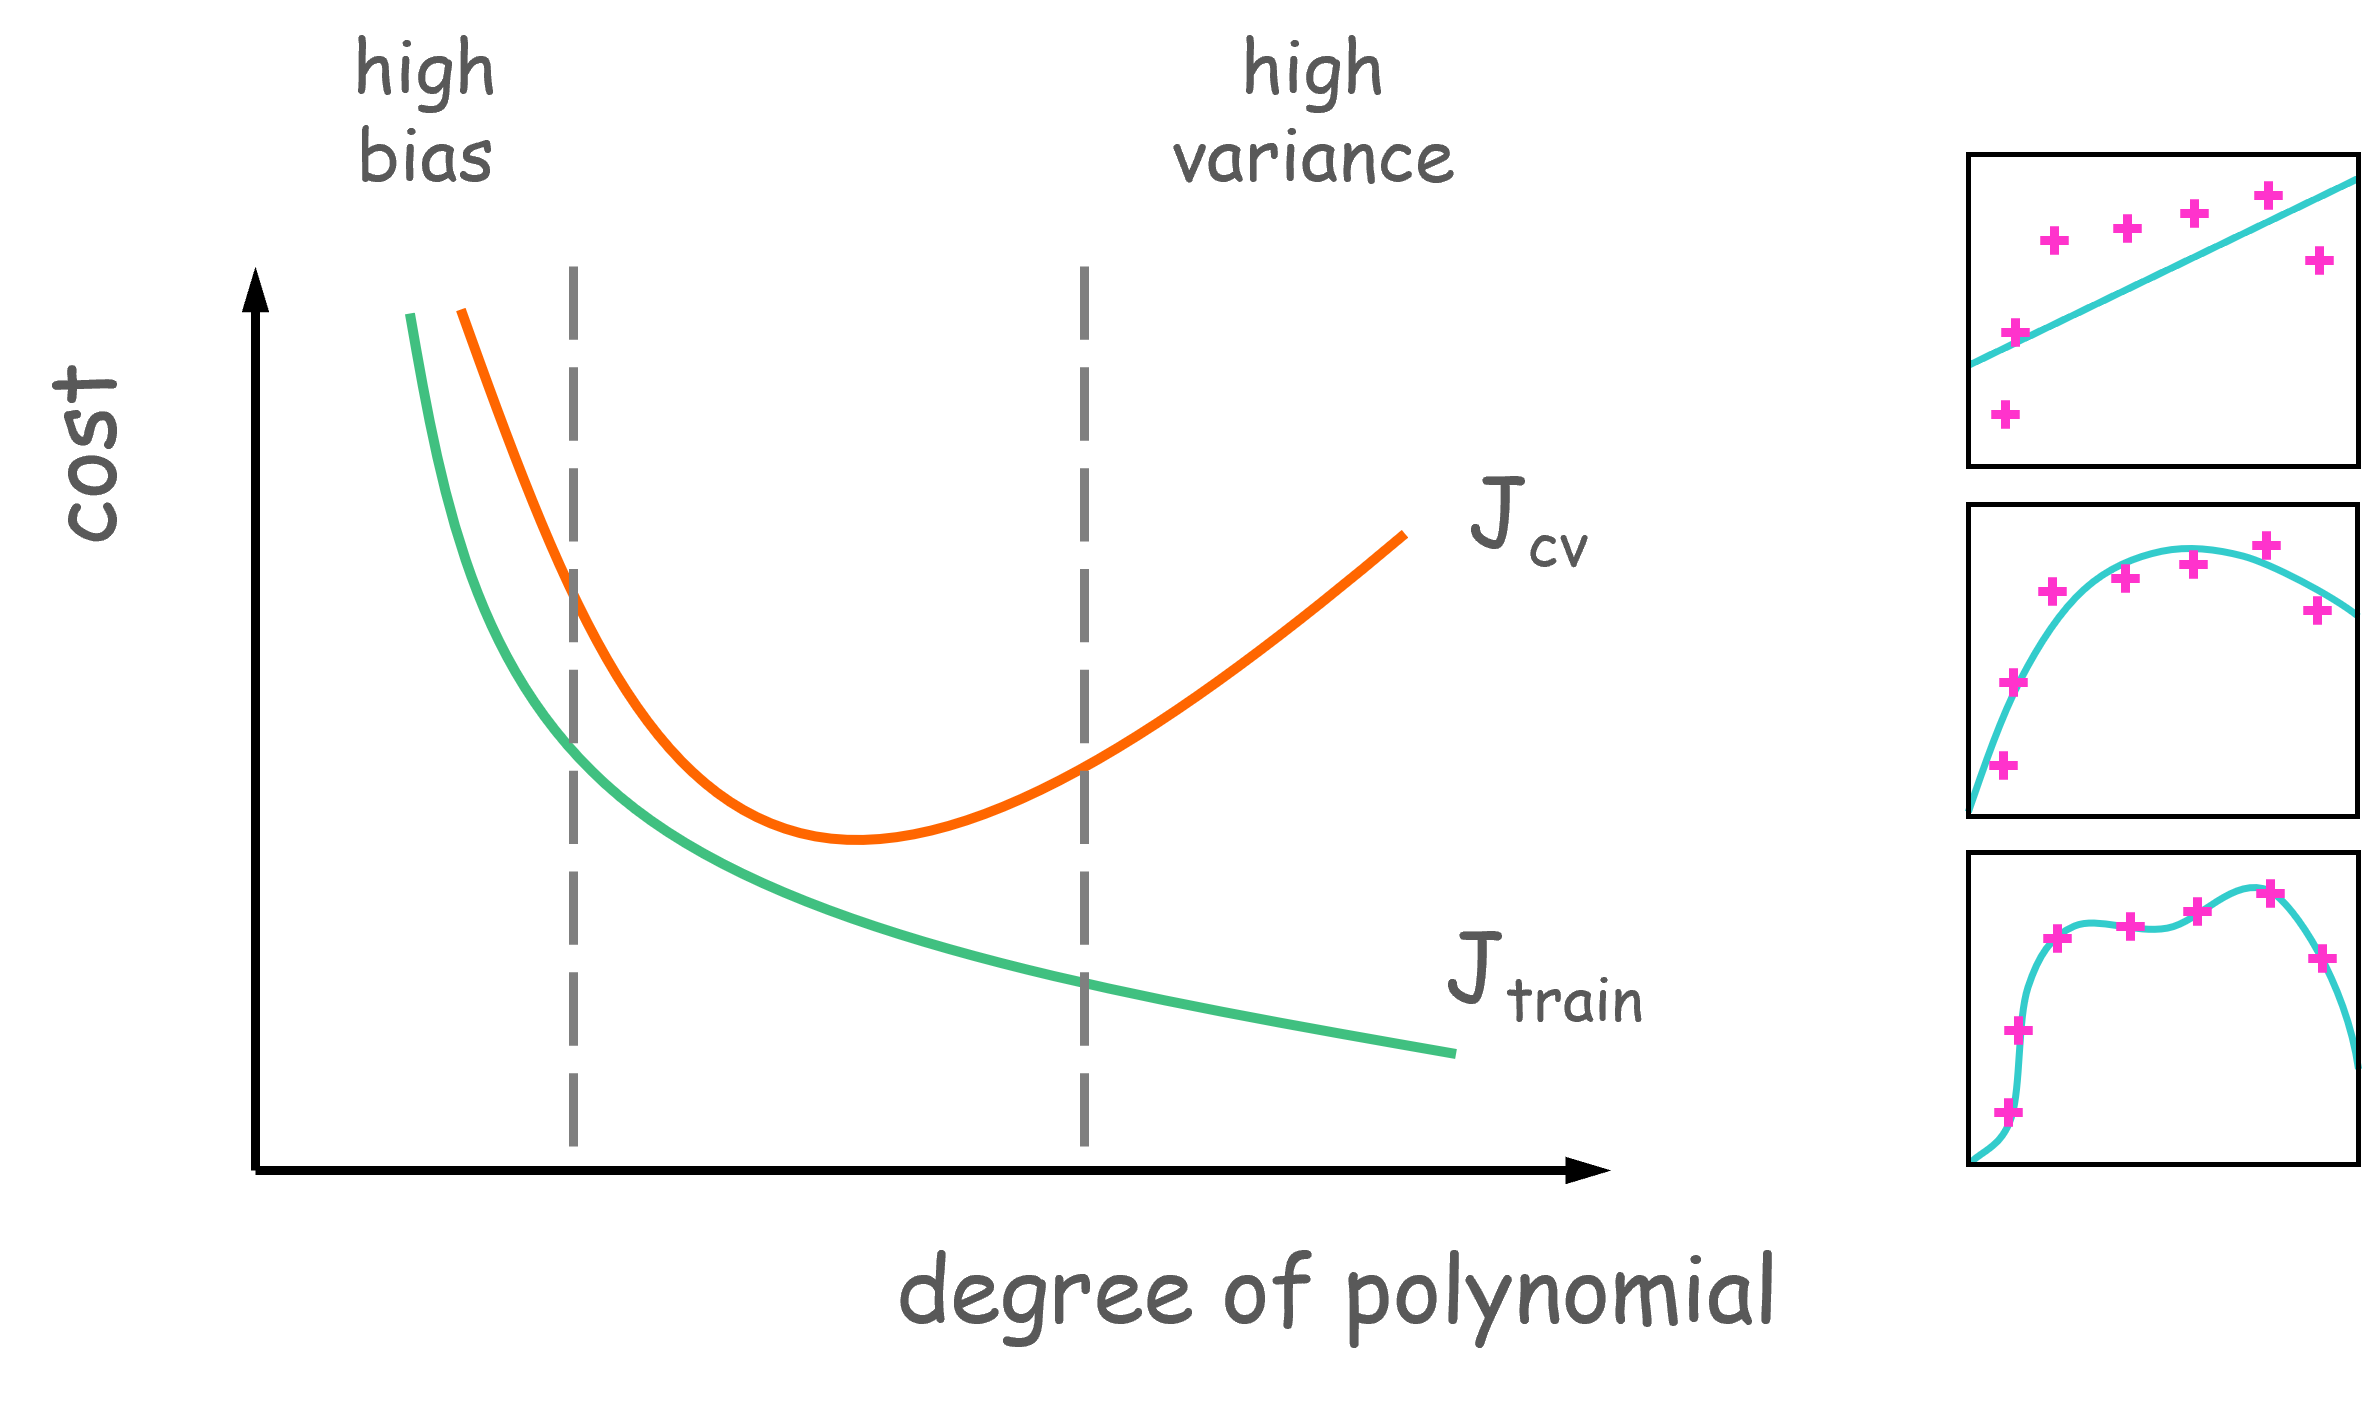
\includegraphics[width=3.8in]{./images/diagnose_degree_of_polynomial.png}
        \caption{Diagnose degree of polynomial $d$}
    \end{figure}

    \item Diagnose regularization parameter
    \begin{figure}[H]
        \centering
        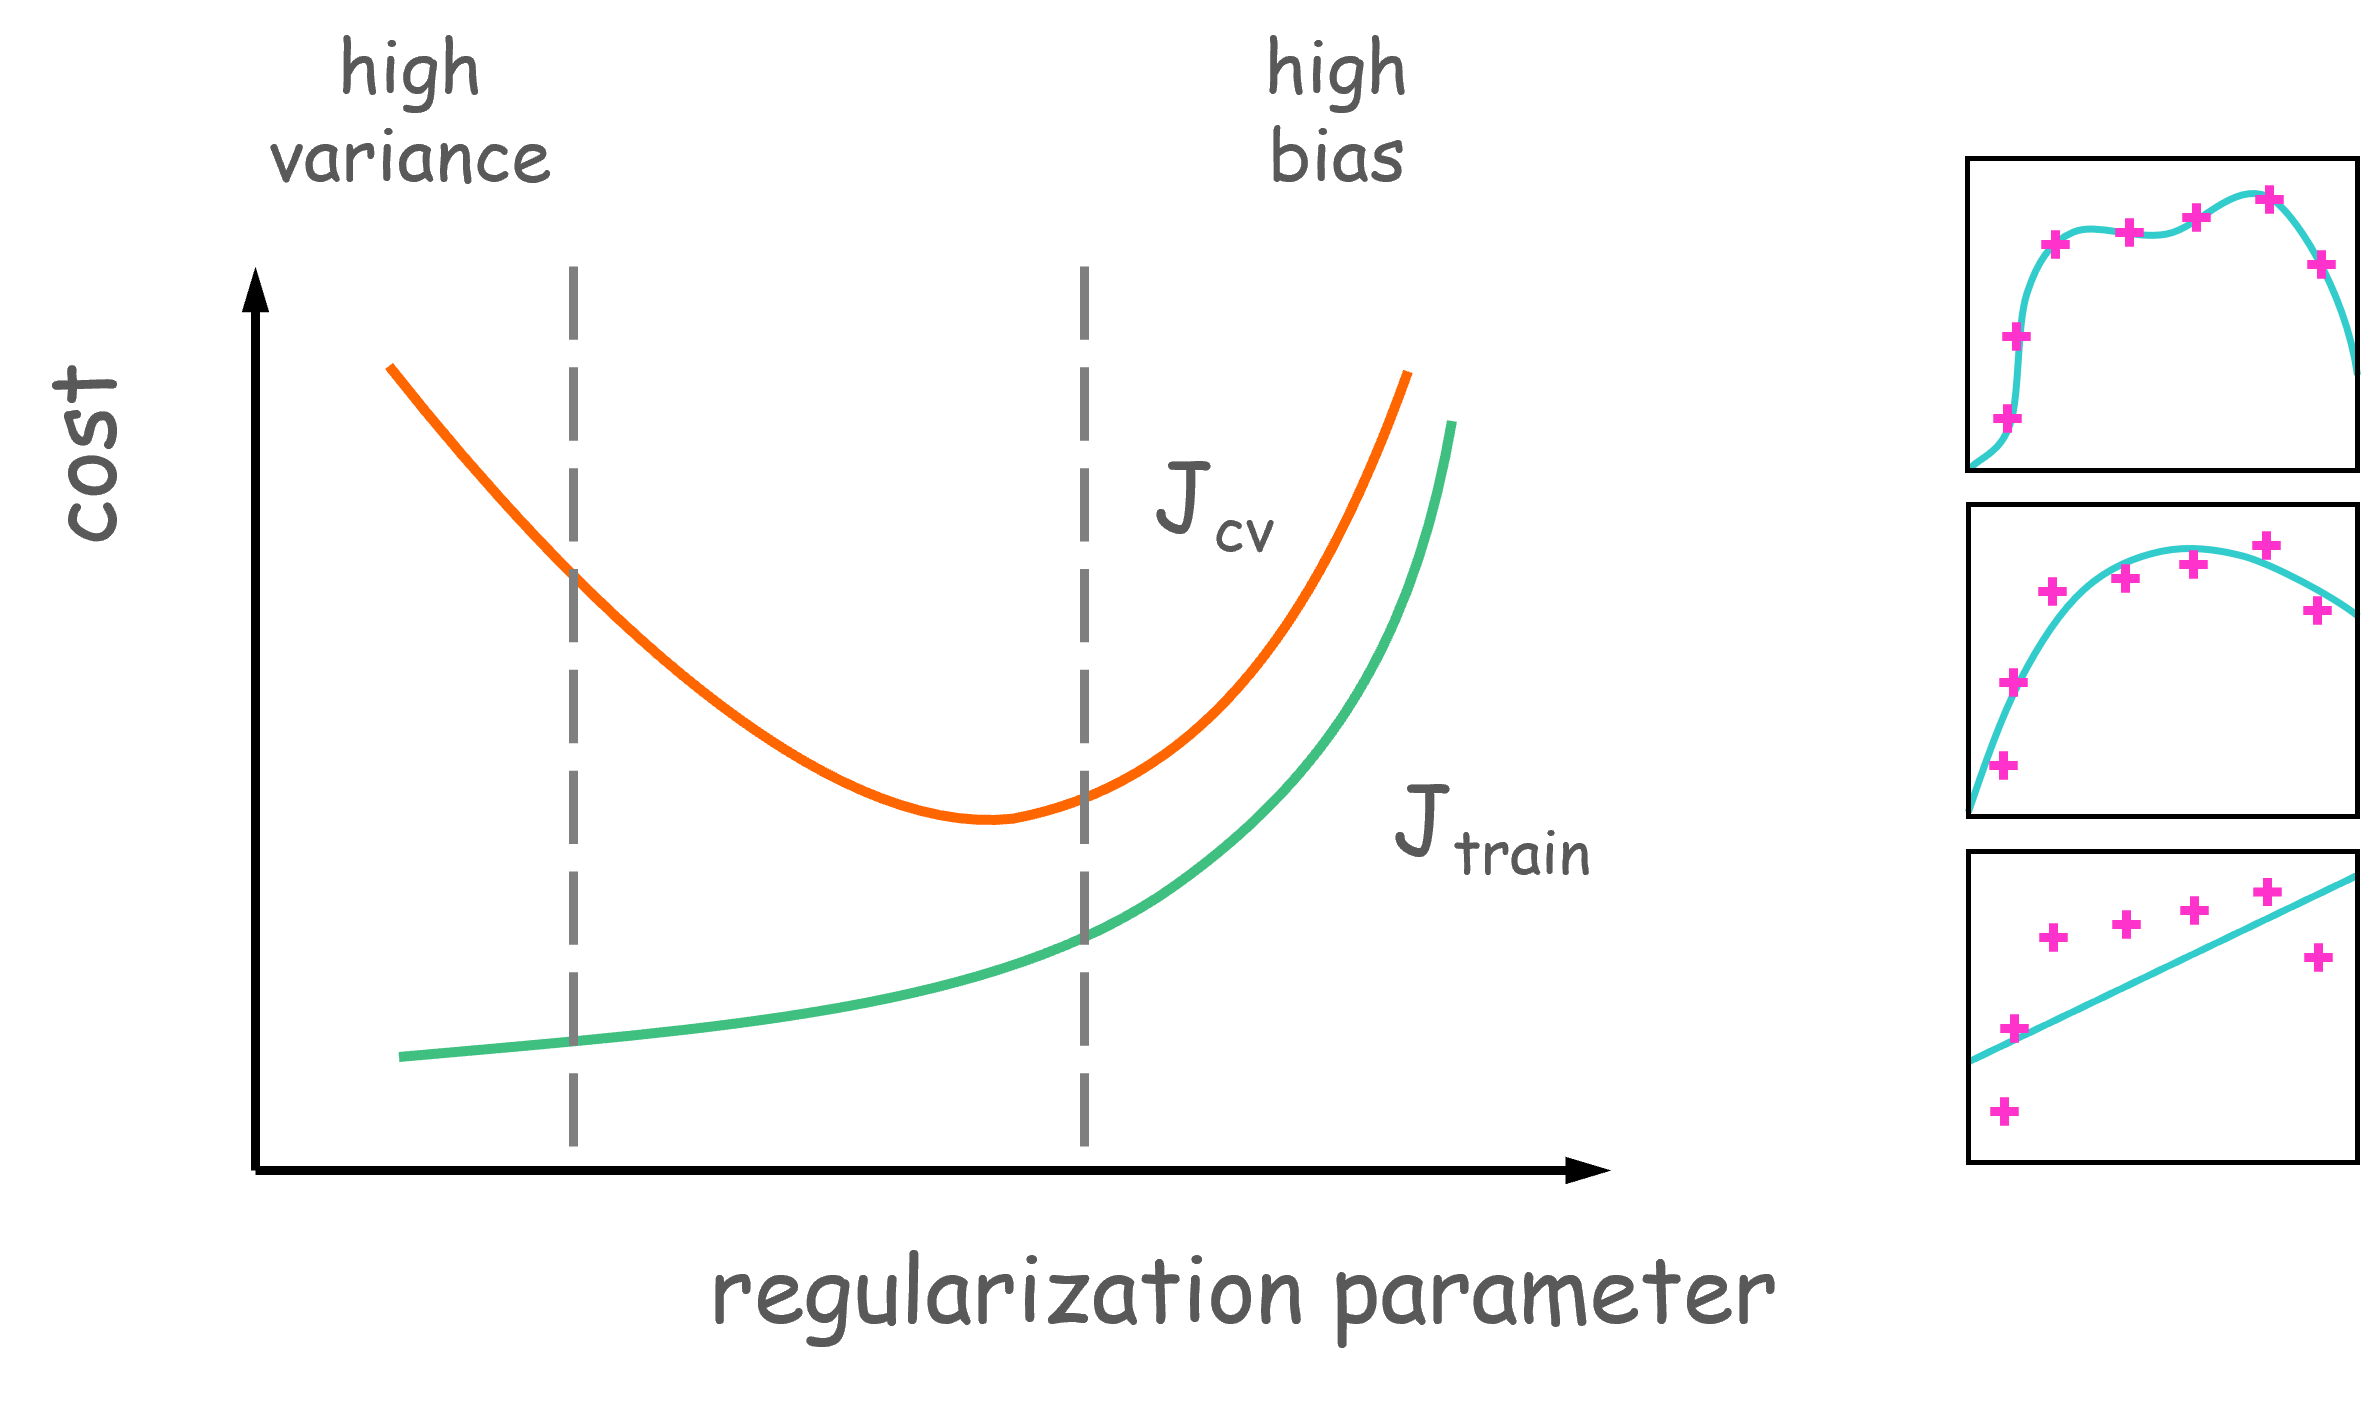
\includegraphics[width=3.8in]{./images/diagnose_regularization_parameter.png}
        \caption{Diagnose regularization parameter $\lambda$}
    \end{figure}

    \item Diagnose training set size
    \begin{figure}[H]
        \centering
        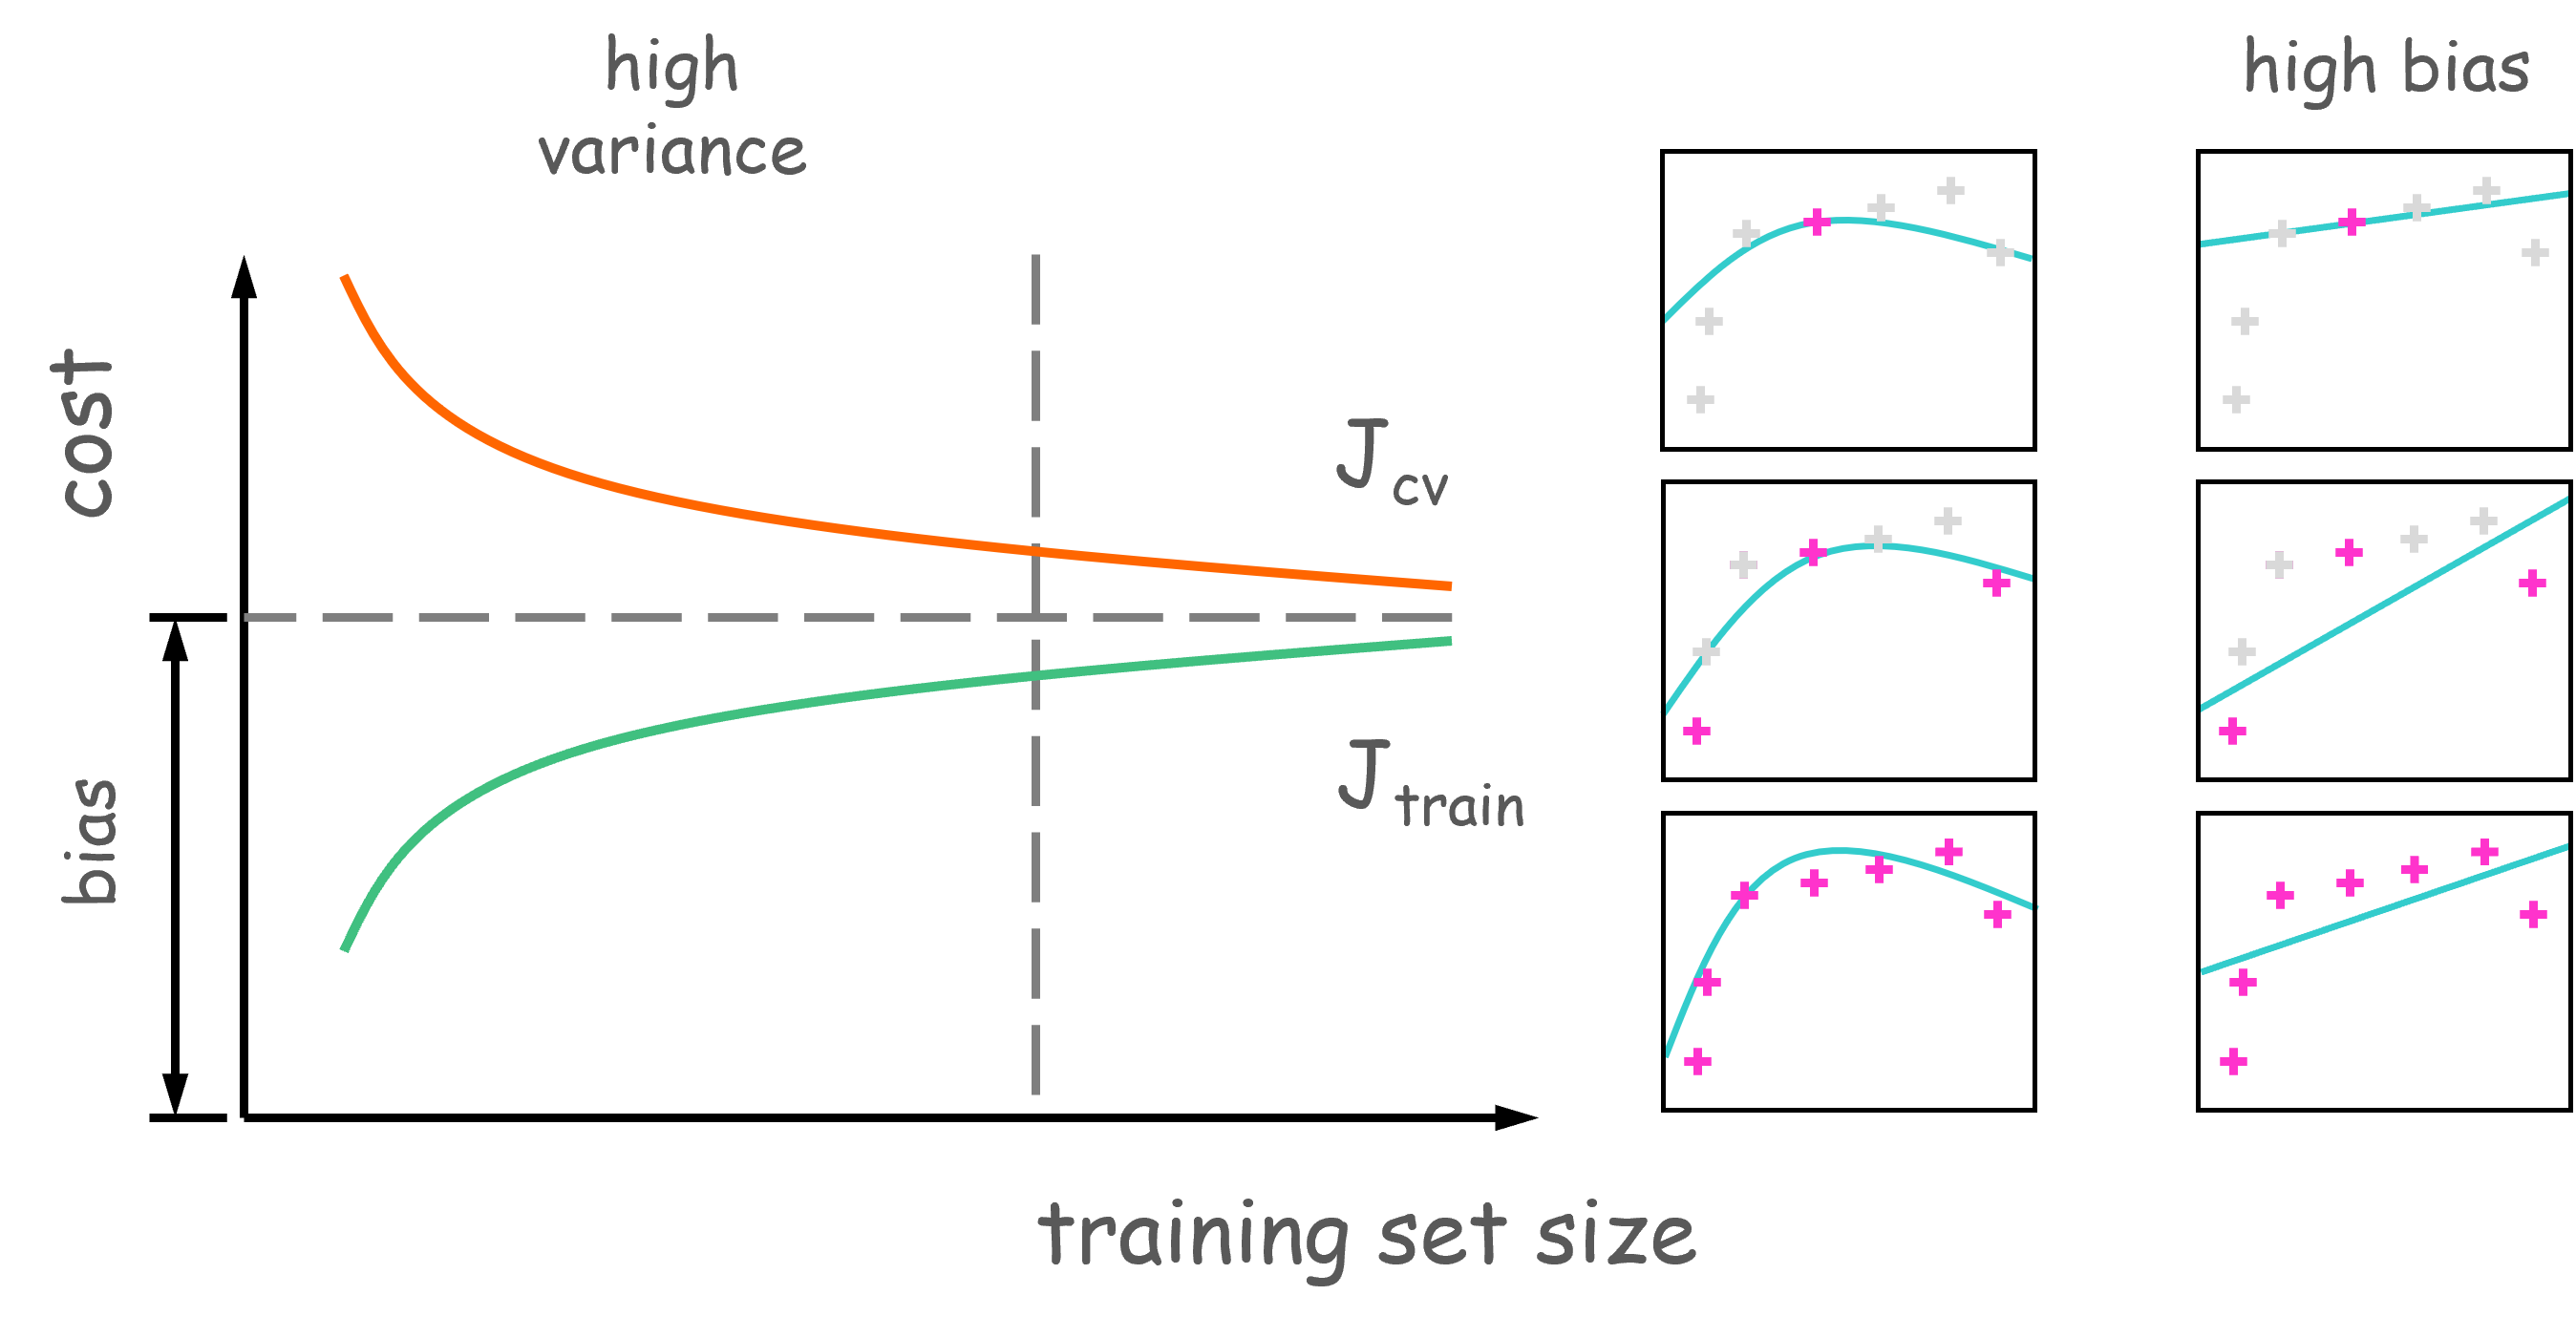
\includegraphics[width=3.8in]{./images/diagnose_training_set_size.png}
        \caption{Diagnose training set size $m$}
    \end{figure}

\end{itemize}


\section{Error analysis}
\begin{itemize}
    \item Define the error metrics
    \begin{table}[H]
        \renewcommand\arraystretch{1.5}
        \caption{Error metrics}
        \centering
        \begin{tabular}{ccc}
            \hline %%%%%%%%%%%%%%%%%%%%%%%%%%%%%%%%%%%%%%%%%
            Cases      & Actual 1       & Actual 0       \\ 
            \hline %%%%%%%%%%%%%%%%%%%%%%%%%%%%%%%%%%%%%%%%%
            Predict 1  & True positive  & False positive \\ 
            Predict 0  & False negative & True negative  \\
            \hline %%%%%%%%%%%%%%%%%%%%%%%%%%%%%%%%%%%%%%%%%
        \end{tabular}
    \end{table}

    \item Define precision $P$ and recall $R$
    \begin{equation}
        \begin{aligned}
            P &= \frac{\text{True pos.}}{\text{True pos.} + \text{False pos.}} \\
            R &= \frac{\text{True pos.}}{\text{True pos.} + \text{False neg.}} \\
        \end{aligned}
    \end{equation}
    
    We want both precision $P$ and recall $R$ could approximate 1, but there is a trade-off between these two values.
    For a higher threshold, the precision $P$ would increase but the recall $R$ would decrease
    \begin{figure}[H]
        \centering
        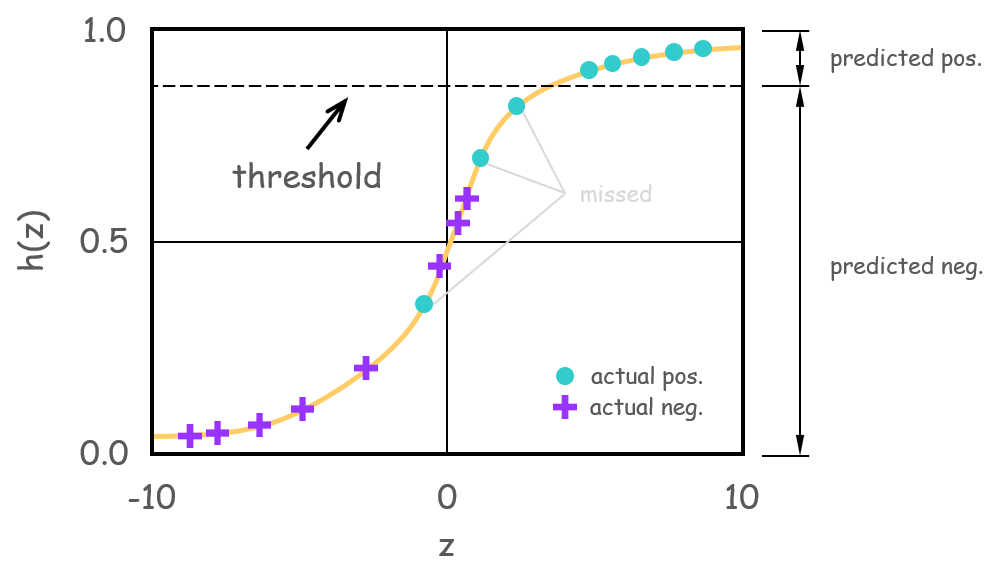
\includegraphics[width=3.8in]{./images/error_highPrecisionLowRecall.png}
        \caption{High precision low recall}
    \end{figure}
    
    \begin{table}[H]
        \renewcommand\arraystretch{1.5}
        \caption{Higher threshold}
        \centering
        \begin{tabular}{lcc}
            \hline %%%%%%%%%%%%%%%%%%%%%%%%%%%%%%%%%%%%%%%%%%%%%%%%%%%%%%%%%%%%%%%%%%%%%%%%%%%%%%%%%%%%
            Cases      & Before ($\text{threshold} = 0.5$)     & After ($\text{threshold} > 0.5$)    \\ 
            \hline %%%%%%%%%%%%%%%%%%%%%%%%%%%%%%%%%%%%%%%%%%%%%%%%%%%%%%%%%%%%%%%%%%%%%%%%%%%%%%%%%%%%
            Precision  & $\frac{7}{7+2} = 0.778$               & $\frac{5}{5+0} = 1.000$             \\ 
            Recall     & $\frac{7}{7+1} = 0.875$               & $\frac{5}{5+3} = 0.625$             \\
            \hline %%%%%%%%%%%%%%%%%%%%%%%%%%%%%%%%%%%%%%%%%%%%%%%%%%%%%%%%%%%%%%%%%%%%%%%%%%%%%%%%%%%%
        \end{tabular}
    \end{table}  
    
    For a lower threshold, the recall $R$ would increase but the precision $P$ would decrease
    \begin{figure}[H]
        \centering
        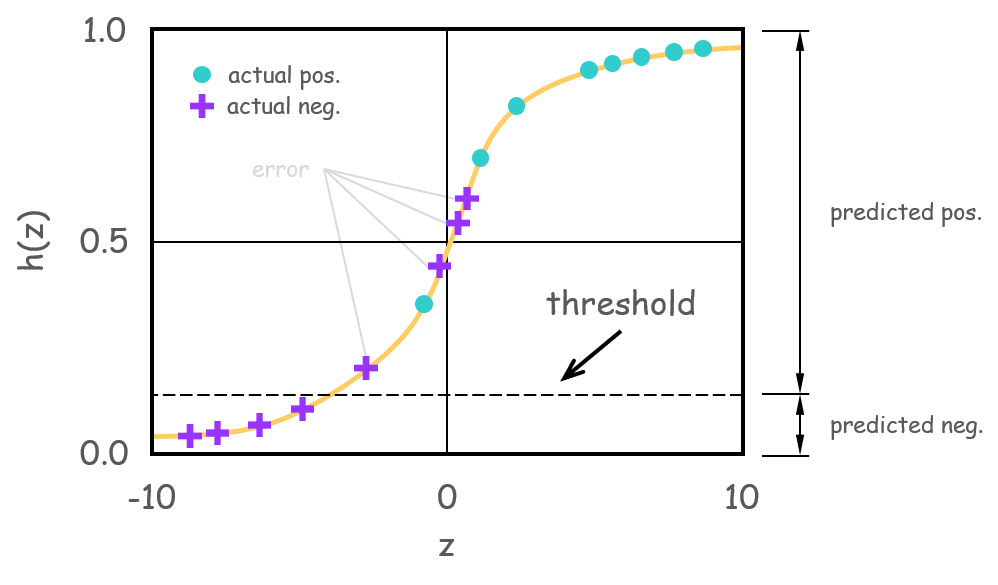
\includegraphics[width=3.8in]{./images/error_lowPrecisionHighRecall.png}
        \caption{Low precision high recall}
    \end{figure}
    
    \begin{table}[H]
        \renewcommand\arraystretch{1.5}
        \caption{Lower threshold}
        \centering
        \begin{tabular}{lcc}
            \hline %%%%%%%%%%%%%%%%%%%%%%%%%%%%%%%%%%%%%%%%%%%%%%%%%%%%%%%%%%%%%%%%%%%%%%%%%%%%%%%%%%%%
            Cases      & Before ($\text{threshold} = 0.5$)     & After ($\text{threshold} < 0.5$)    \\ 
            \hline %%%%%%%%%%%%%%%%%%%%%%%%%%%%%%%%%%%%%%%%%%%%%%%%%%%%%%%%%%%%%%%%%%%%%%%%%%%%%%%%%%%%
            Precision  & $\frac{7}{7+2} = 0.778$               & $\frac{8}{8+4} = 0.667$             \\ 
            Recall     & $\frac{7}{7+1} = 0.875$               & $\frac{8}{8+0} = 1.000$             \\
            \hline %%%%%%%%%%%%%%%%%%%%%%%%%%%%%%%%%%%%%%%%%%%%%%%%%%%%%%%%%%%%%%%%%%%%%%%%%%%%%%%%%%%%
        \end{tabular}
    \end{table}  
    
    \item The F-score or F-measure is a measure of a test's accuracy. It is calculated from the precision and recall of the test,
    \begin{equation}
        F_1 = 2 \frac{PR}{P+R}
    \end{equation}
    
    This is better than using an average equation like $\frac{P+R}{2}$.
    

\end{itemize}

 
    \chapter{Support Vector Machine}


\section{Introduction}
\begin{itemize}
    \item The cost of the $i^{th}$ item in the logistic function is
    \begin{equation} J^{(i)} = y^{(i)} \log{h^{(i)}} + (1-y^{(i)}) \log{(1-h^{(i)})} \end{equation}
    where
    \begin{equation} h^{(i)} = \frac{1}{1+e^{-\mathbf{z}}} \end{equation}
    
    \item Plot the cost functions as $y=1$ and $y=0$. SVM use the approximated costs named as $L_1$ and $L_0$.
    \begin{figure}[!htbp]
        \begin{minipage}[t]{0.5\textwidth}
            \centering
            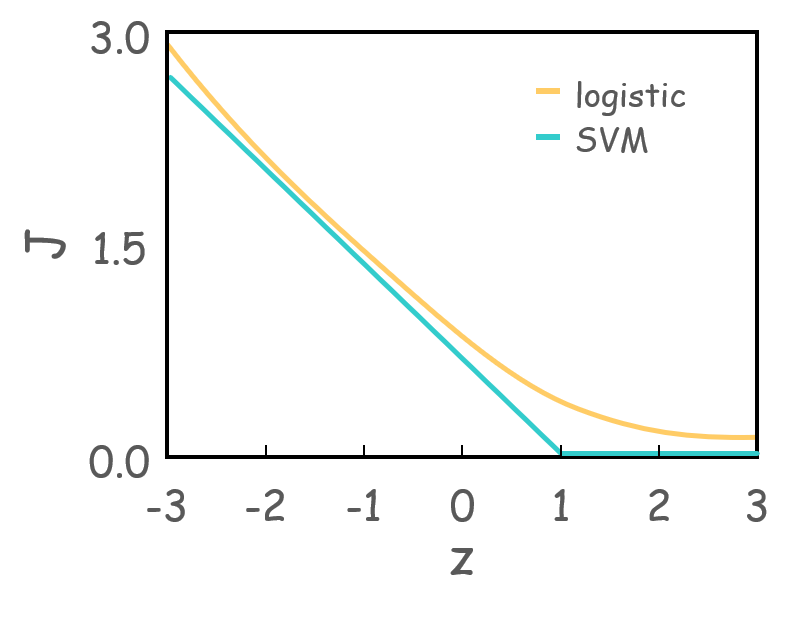
\includegraphics[width=2.0in]{./images/supportVectorMachineY1.png}
            \caption{The cost function as $y=1$}
        \end{minipage}
        \begin{minipage}[t]{0.45\textwidth}
            \centering
            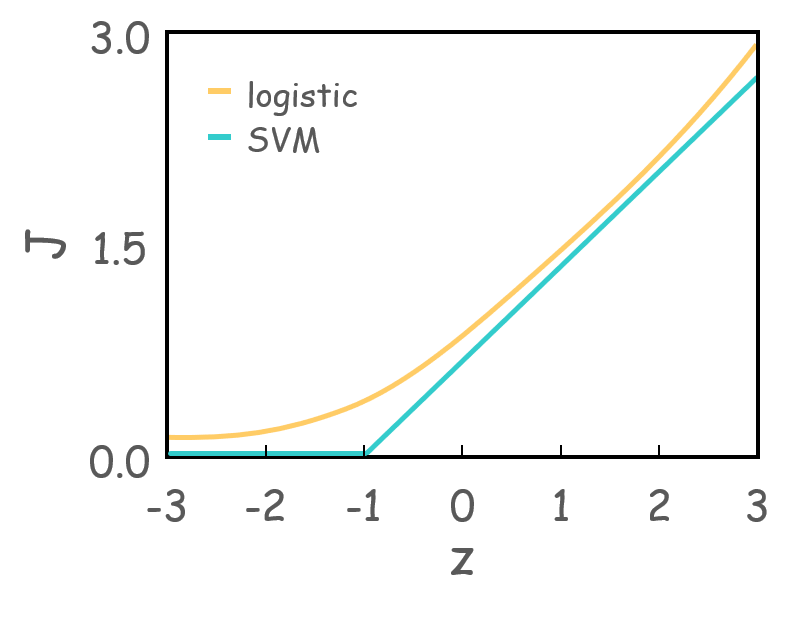
\includegraphics[width=2.0in]{./images/supportVectorMachineY0.png}
            \caption{The cost function as $y=0$}
        \end{minipage}
    \end{figure}
\end{itemize}


\section{The optimization of the cost function}
\begin{itemize}
\item The object of the optimization is
\begin{equation} \min_\theta \frac{1}{m} \sum_{i=0}^{m} \left[y^{(i)} L_1(z^{(i)}) + (1-y^{(i)}) L_0(z^{(i)}) \right] + \frac{\lambda}{2m} \sum_{j=1}^{n} \theta_j^2 \end{equation}
As $z^{(i)} = \mathbf{x}^{(i)}\theta$. When $z^{(i)} \geq 1$ or $z^{(i)} \leq -1$, the first term in the cost is zero, only the regularization term will remain.
As a result, the total cost would only remain
\begin{equation} \min_\theta \sum_{j=1}^{n} \theta_j^2 \end{equation}

And that is to say
\begin{equation}
    \min_\theta \sum_{j=1}^{n} \theta_j^2 = \min_\theta{\left\|\theta\right\|}^2 = \min_\theta{\left\|\theta\right\|}
\end{equation}

\item Observe $\mathbf{x}^{(i)}\theta$. This can be seen as an inner product of two vectors $\theta$ and $\mathbf{x}^{(i)}$. Where
\begin{equation} \theta = \left[{\begin{matrix} \theta_0 & \theta_1 & \dots & \theta_n \end{matrix}}\right]^T \end{equation}
\begin{equation} \mathbf{x}^{(i)} = \left[{\begin{matrix} x_0^{(i)} & x_1^{(i)} & \dots & x_n^{(i)} \end{matrix}}\right] \end{equation}
Assum the angle between $\theta$ and $\mathbf{x}^{(i)}$ is $\varphi^{(i)}$. That is to say
\begin{equation}
    \begin{aligned}
        \mathbf{x}^{(i)}\theta &= \left\| \mathbf{x}^{(i)} \right\| \left\| \theta \right\| \cos\varphi^{(i)} \\
                               &= p^{(i)} \left\| \theta \right\| \sign\varphi^{(i)}
    \end{aligned}
\end{equation}
Where $p^{(i)}$ is the projection of $\mathbf{x}^{(i)}$ onto $\theta$

\item Now the question is how to minimize the cost function. In cases of margin classification. The following must be satisfied
\begin{equation}
    \left\{ \begin{aligned}
        \mathbf{x}^{(i)}\theta &= \left\| \theta \right\| p^{(i)} &\geq 1 & \text{, for } x^{(i)}\\
        \mathbf{x}^{(j)}\theta &= -\left\| \theta \right\| p^{(j)} &\leq 1 & \text{, for } x^{(j)}\\
    \end{aligned} \right.
\end{equation}
It's obvious to see that as $p^{(i)}$ and $p^{(j)}$ get larger, a smaller $\| \theta \|$ would be needed to satisfy the inequality.
That implies \emph{when $\theta$ in the direcction to make a maximized margin, then the total cost would be minimized.}
\begin{figure}[!htbp]
    \centering
    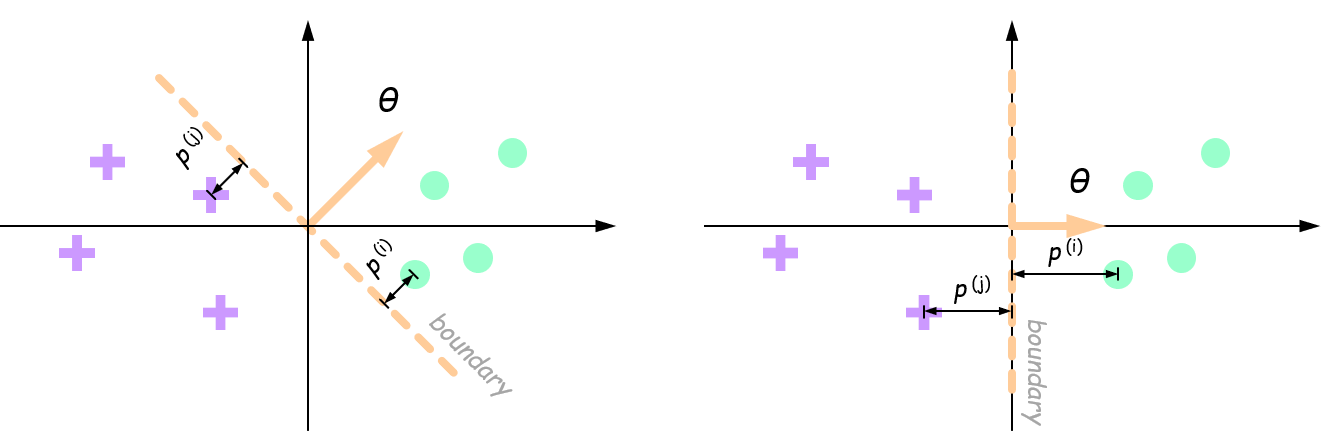
\includegraphics[width=4.8in]{./images/marginClassification.png}
    \caption{Margin classification with different $\theta$}
\end{figure}
\end{itemize}


\section{Gaussian kernel}
\begin{itemize}
\item Gaussian kernel can make prediction of input data with a non-linear decision boundary. Given $m$ data, then choose these data as landmarks.
\begin{equation}
    \begin{array}{cccc}
        l^{(1)} = x^{(1)} & l^{(2)} = x^{(2)} & \dots & l^{(m)} = x^{(m)}
    \end{array}
\end{equation}

\item Define the \emph{similarity function}
\begin{equation}
    \begin{aligned}
        f_{j}^{(i)} &= f(x^{(i)}, l^{(j)}) \\
        &= \exp\left({-\frac{\left\|x^{(i)} - l^{(j)}\right\|^2}{2\sigma^2}}\right)
    \end{aligned}
\end{equation}
Then the values of the similarity fuctions would be
\begin{equation}
    f_{j}^{(i)} \approx
    \left\{\begin{aligned}
        1 &\text{, for } x^{(i)} \approx l^{(j)}\\
        0 &\text{, for } x^{(i)} \neq l^{(j)}\\
    \end{aligned}\right.
\end{equation}
\begin{figure}[!htbp]
    \centering
    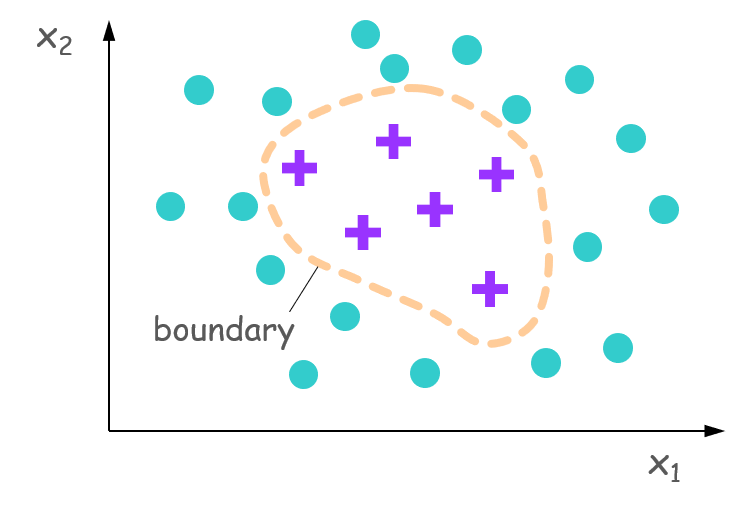
\includegraphics[width=2.8in]{./images/nonlinearDecisionBoundary.png}
    \caption{Non-linear decision boundary}
\end{figure}

\item For each similarity functions, its distribution looks like
\begin{figure}[!htbp]
    \centering
    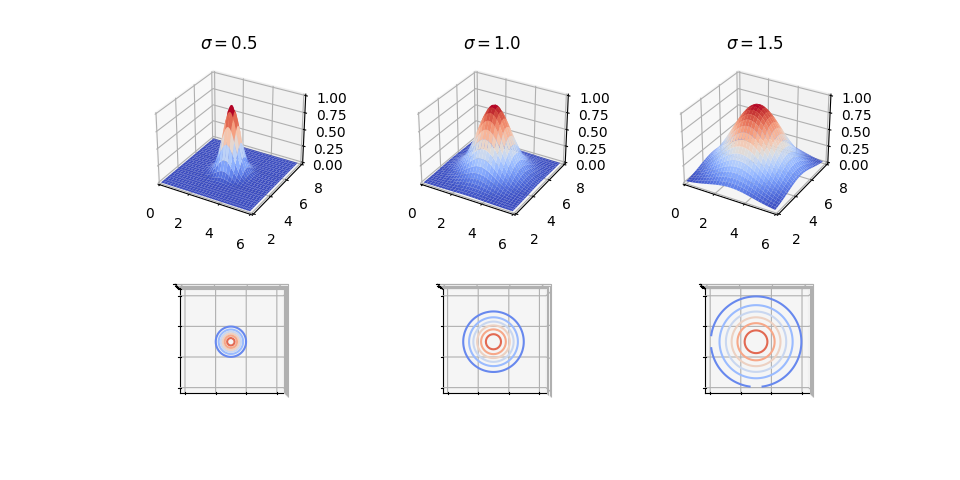
\includegraphics[width=7.0in]{./images/gaussianKernel.png}
    \caption{Gaussian kernel functions}
\end{figure}

\item For training example $x^{(i)}$, all of its similarity would be
\begin{equation}
    \mathbf{f}^{(i)} = \left[\begin{matrix}
        f_0^{(i)} \\ f_1^{(i)} \\ f_2^{(i)} \\ \vdots \\ f_m^{(i)}
    \end{matrix}\right] = 
    \left[\begin{matrix}
        1 \\ f(x^{(i)}, l^{(1)}) \\ f(x^{(i)}, l^{(2)}) \\ \vdots \\ f(x^{(i)}, l^{(m)})
    \end{matrix}\right]
\end{equation}
The $i^{th}$ item in the array is
\begin{equation}
    f_i^{(i)} = f(x^{(i)}, l^{(i)}) = 1
\end{equation}

\item So, how does Gaussian kernel work? Assume
\begin{equation}
    z^{(i)} = \theta^T\mathbf{f}^{(i)}
\end{equation}

Put $z^{(i)}$ to the sigmoid function.
\begin{equation}
    g^{(i)} = \frac{1}{1+e^{-z^{(i)}}}
\end{equation}

Then the decision boundary would be
\begin{equation}
    \begin{split}
        z^{(i)} = \theta^T \mathbf{f}^{(i)} & \geq 0 \Rightarrow g^{(i)} \geq 0.5 \Rightarrow y^{(i)} = 1\\
        z^{(i)} = \theta^T \mathbf{f}^{(i)} & <    0 \Rightarrow g^{(i)} <    0.5 \Rightarrow y^{(i)} = 0
    \end{split}
\end{equation}

Then the total cost become
\begin{equation}
    \min_\theta \frac{1}{m} \sum_{i=0}^{m} \left[{y^{(i)} L_1(z^{(i)}) + (1-y^{(i)}) L_0(z^{(i)}) }\right] + \frac{\lambda}{2m} \sum_{j=1}^{m} \theta_j^2
\end{equation}
\end{itemize}


    \chapter{K-means Algorithm}


\section{Introduction}
\begin{itemize}
    \item Randomly initialize $K$ cluster centroids. Normally, $K$ \emph{training example} were picked and treated as the initial clusters. 
    \begin{equation}
        \mu_k \in \mathbb{R}^n \text{ , for } k=1,2,\dots,K
    \end{equation}
    
    \item Find the closet cluster for each $x^{(i)}$ and 
    partition the $m$ observations into $K$ sets according to their closet cluster
    \begin{equation}
        \textbf{S} = \left\{S_1, S_2, \dots, S_K\right\}
    \end{equation}
    
    \item Find the center of geometry (mean) and then assign this value as a new $\mu_k$ for next iteration

    \begin{figure}[!htbp]
        \begin{minipage}[t]{0.5\textwidth}
            \centering
            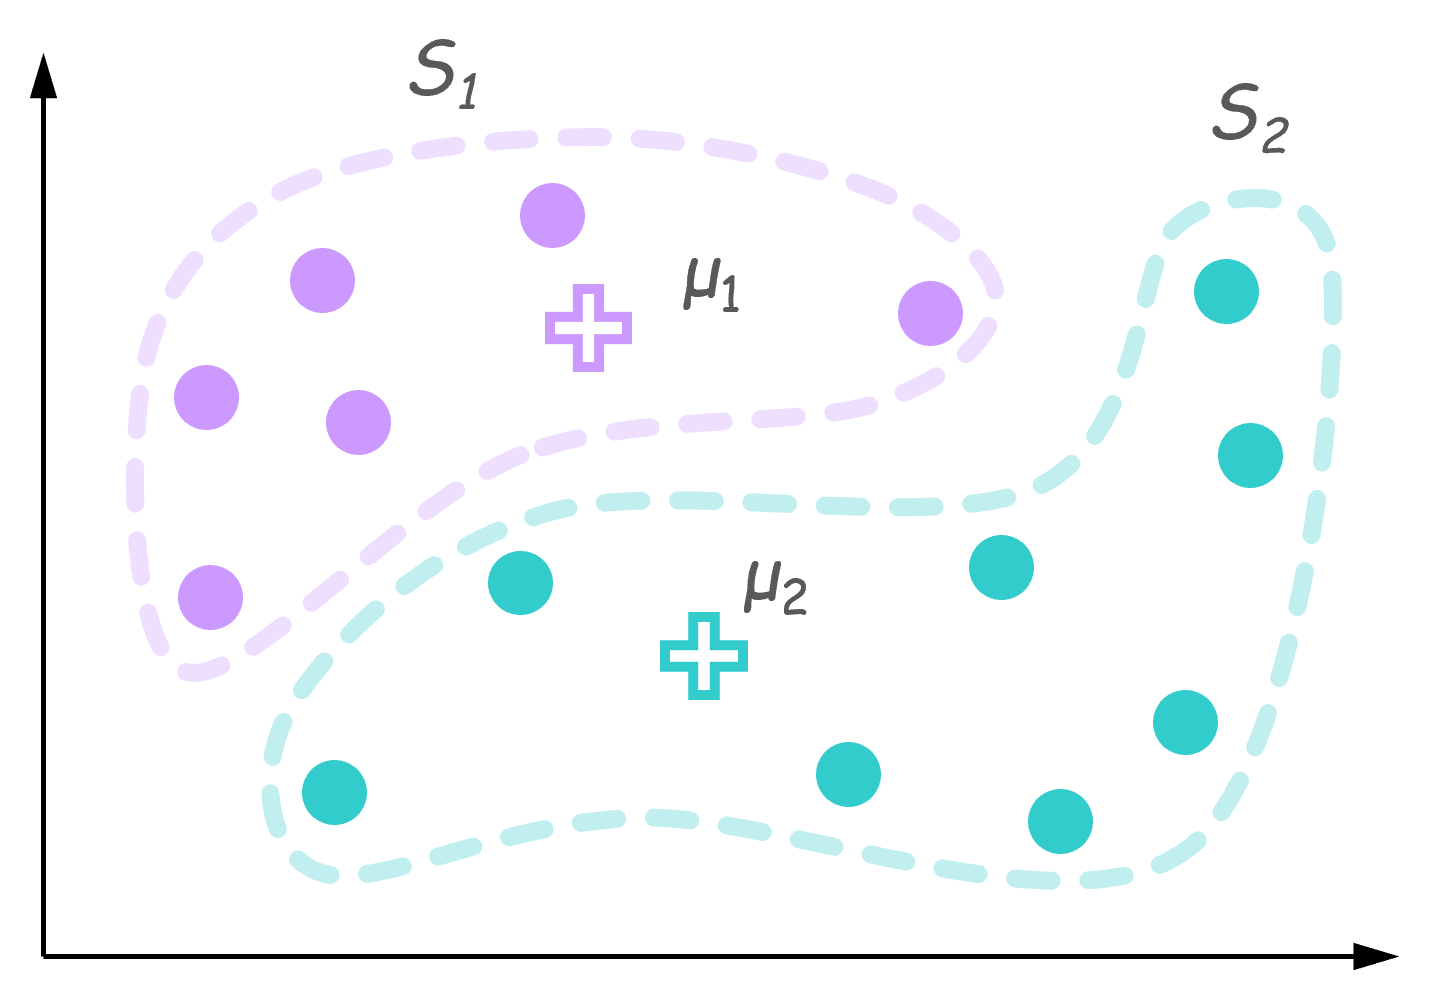
\includegraphics[width=2.2in]{./images/kClusterInitial.png}
            \caption{Initial cluster centroids}
        \end{minipage}
        \begin{minipage}[t]{0.45\textwidth}
            \centering
            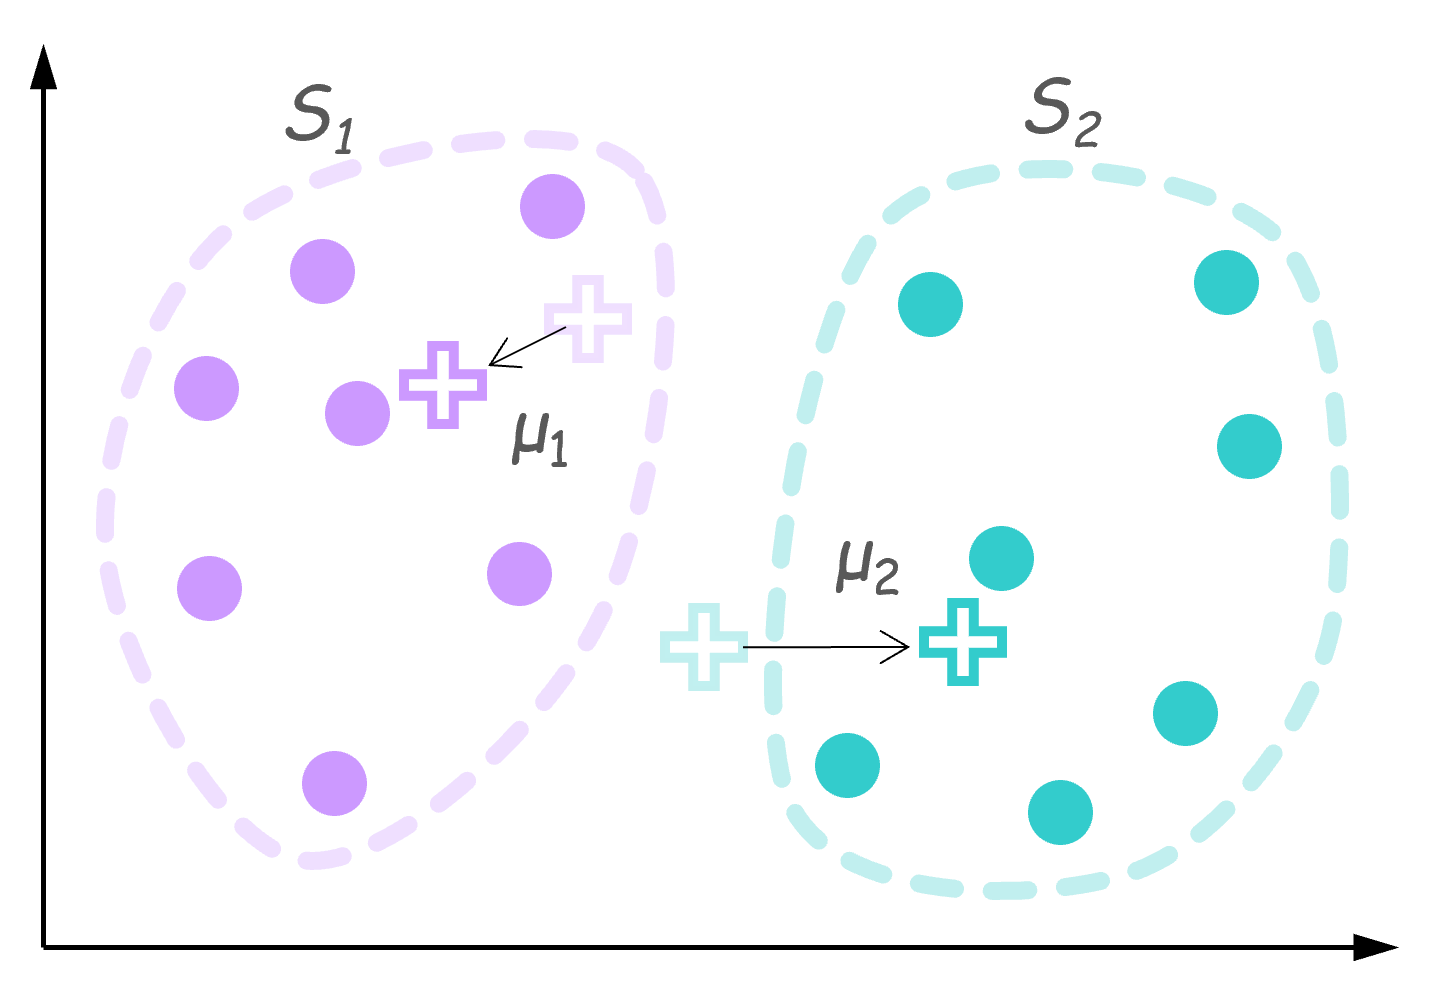
\includegraphics[width=2.2in]{./images/kClusterIter.png}
            \caption{Cluster centroids at first iteration}
        \end{minipage}
    \end{figure}
    
    \item Optimization objective
    \begin{equation}
        \mathop{\arg\min}\limits_{\textbf{S}} \sum_{k=1}^{K} \sum_{x^{(i)} \in S_i}\left\lVert {x^{(i)} - \mu_k} \right\rVert ^2
    \end{equation}
\end{itemize}


\section{Choosing the number of clusters}
\begin{itemize}
    \item Actually, there isn't a great way to choose the number of clusters automatically. 
    By far, the most common way is still choosing it manually by looking at visualizations or by looking at the output of the clustering algorithm.
    \item One common method is Elbow Method. The intuition is that increasing the number of clusters will naturally improve the fit.
    Once the line chart resembles an arm, then the ``elbow'' (the point of inflection on the curve) is a good indication that the underlying model fits best at that point.
    \begin{figure}[!htbp]
        \centering
        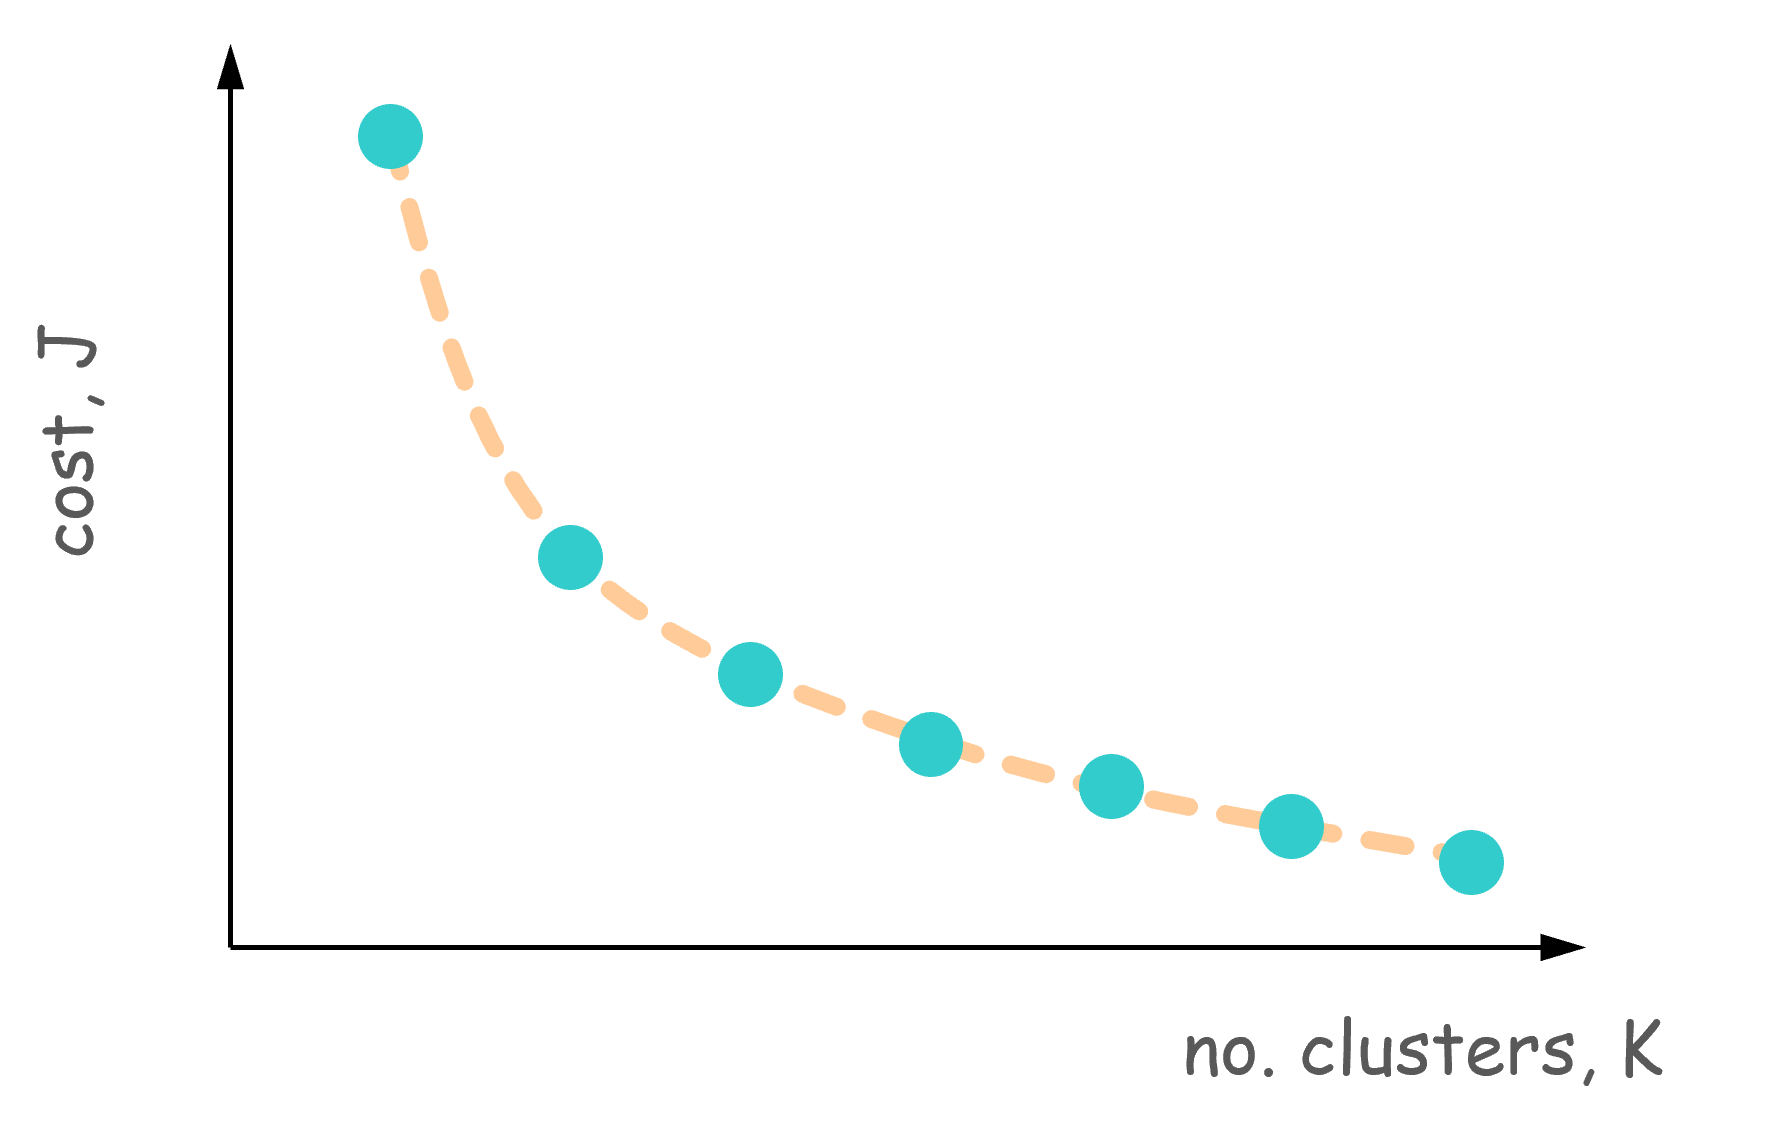
\includegraphics[width=3.2in]{./images/elbowMethod.png}
        \caption{The cost value differ with the number of clusters}
    \end{figure}
\end{itemize}

    \chapter{Principal Component Analysis}


\section{Introduction}
\begin{itemize}
    \item Dimensionality Reduction

    \begin{figure}[!htbp]
        \begin{minipage}[t]{0.45\textwidth}
            \centering
            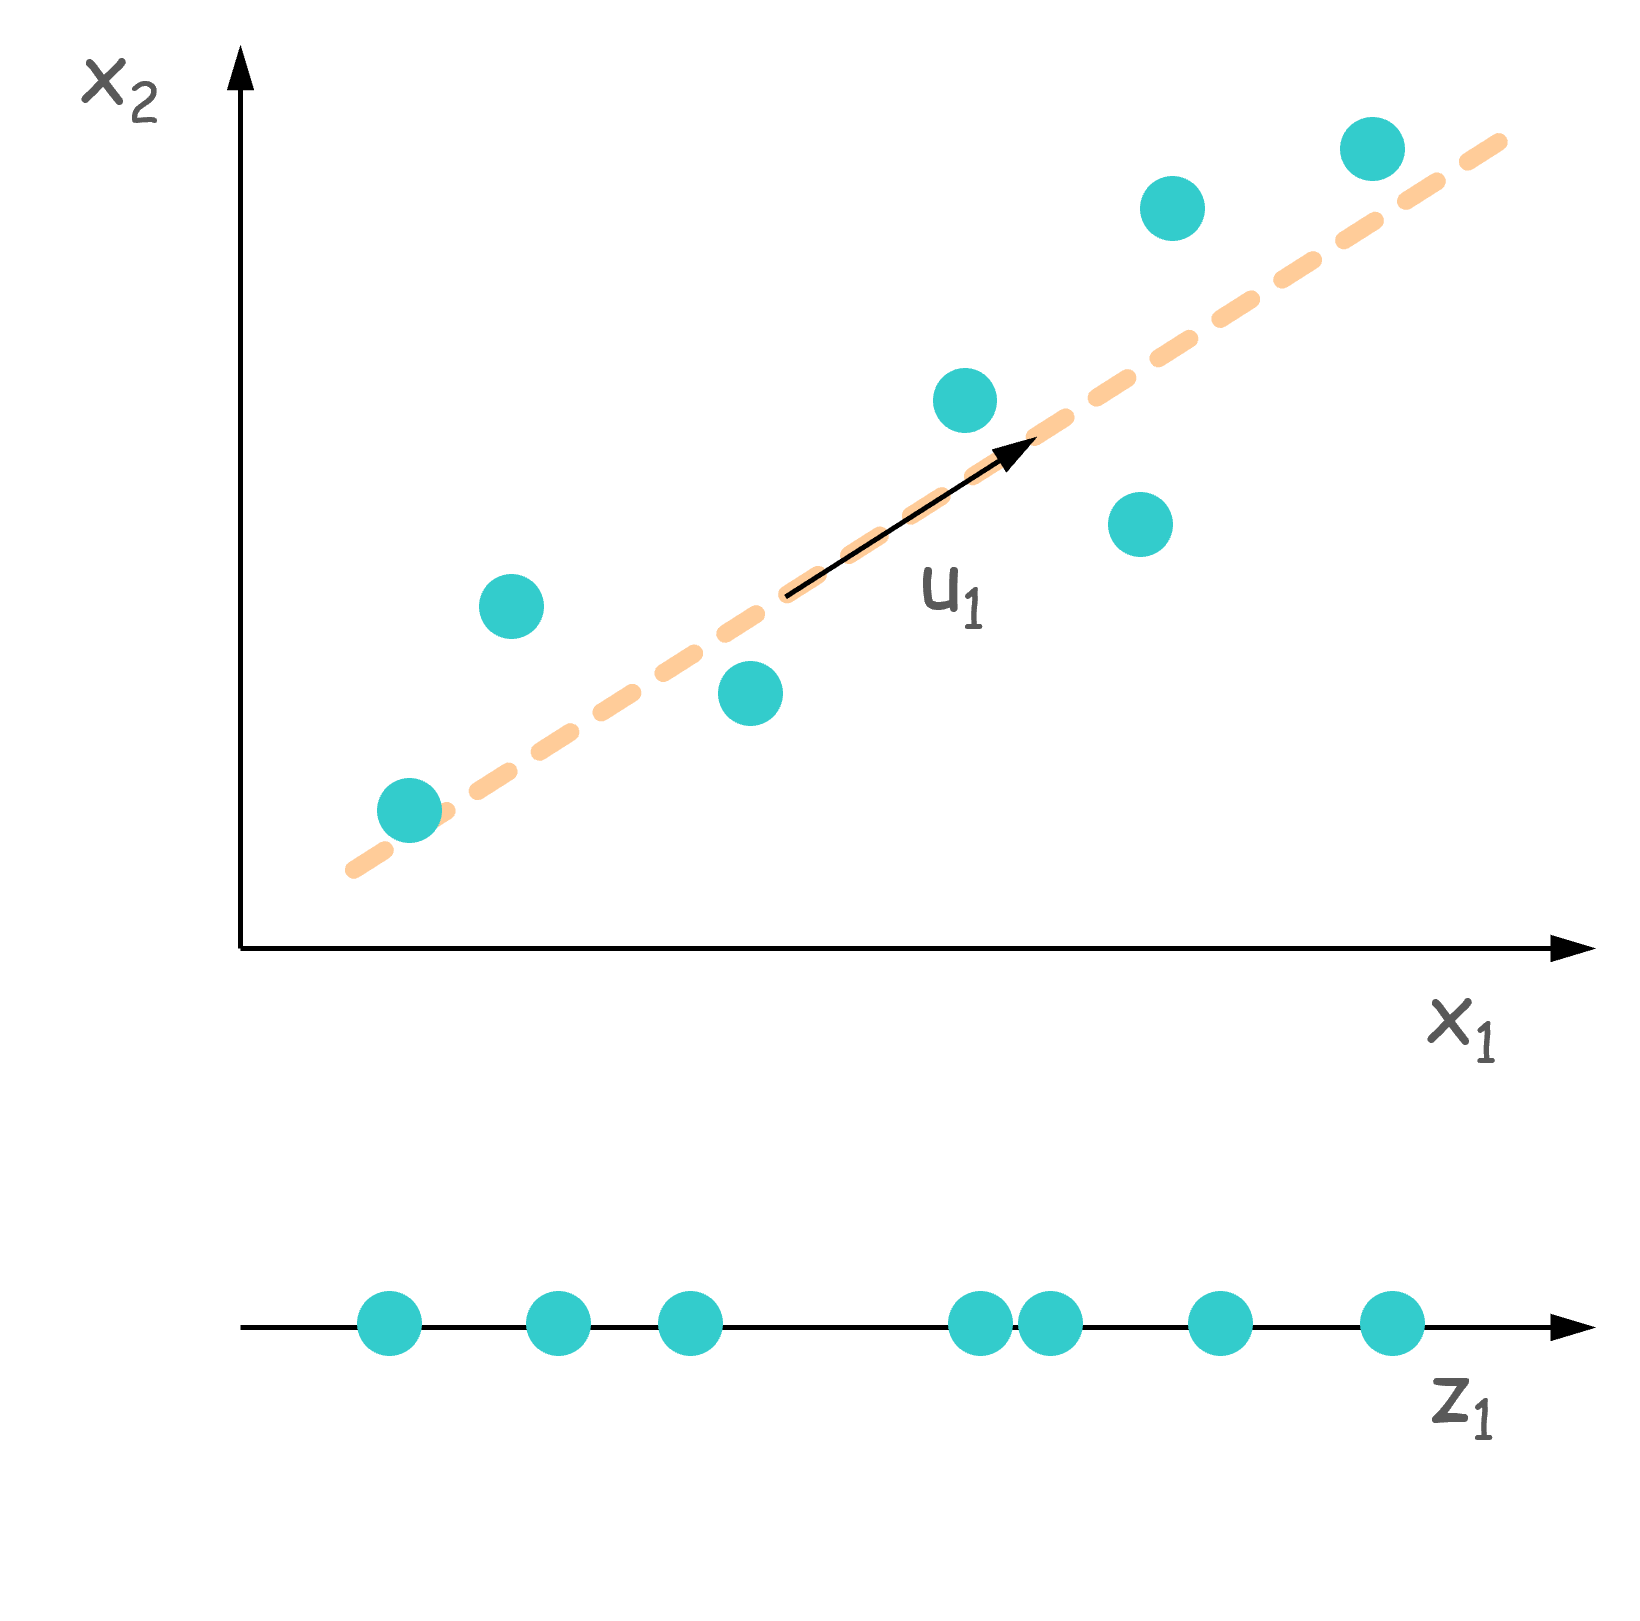
\includegraphics[width=2.2in]{./images/dimensionalityReduction2D.png}
            \caption{Reduction from 2D to 1D}
        \end{minipage}
        \begin{minipage}[t]{0.45\textwidth}
            \centering
            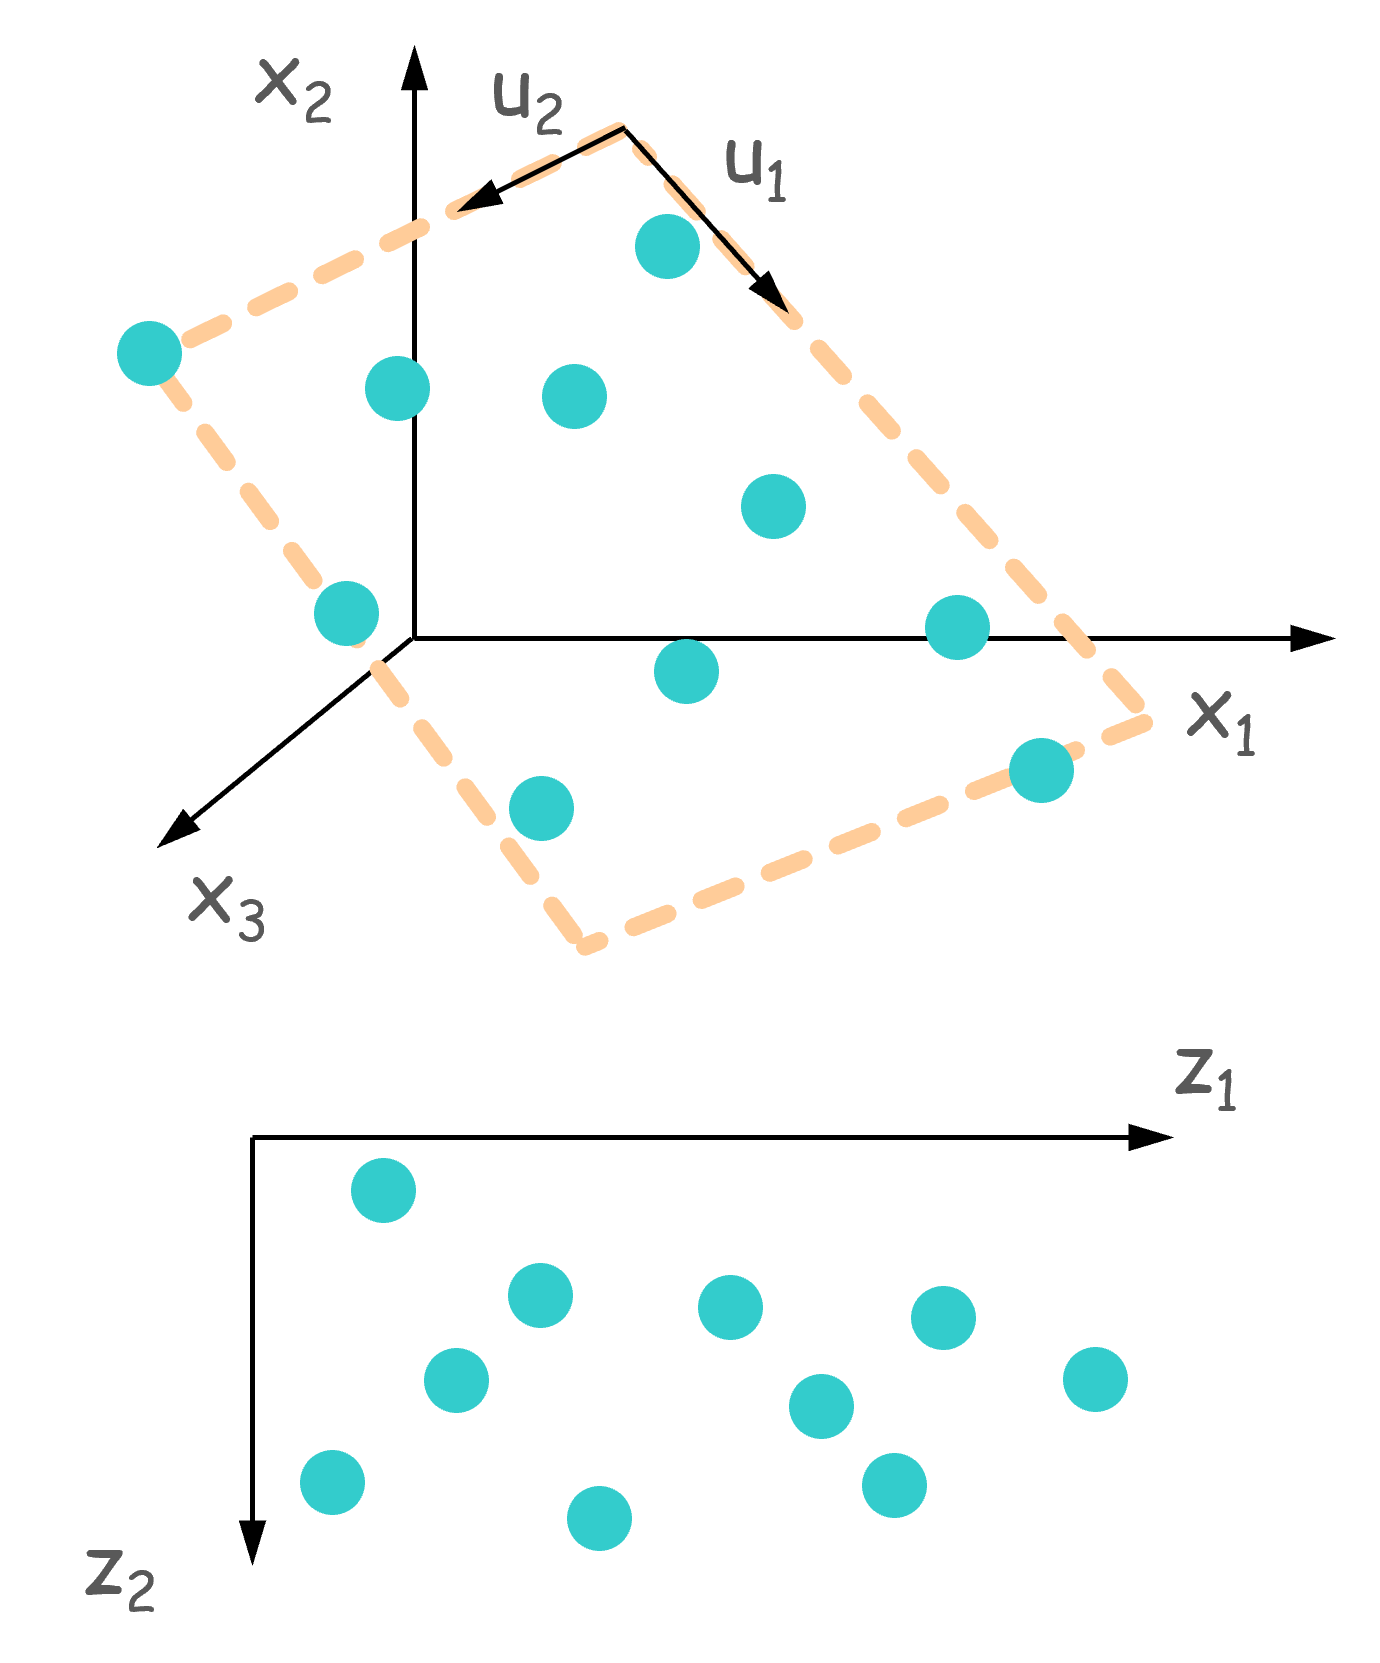
\includegraphics[width=2.2in]{./images/dimensionalityReduction3D.png}
            \caption{Reduction from 3D to 2D}
        \end{minipage}
    \end{figure}

    \item To reduce training data from n­‐dimension to k­‐dimension, find $k$ vectors
    \begin{equation}
        u^{(1)}, u^{(2)}, \dots, u^{(k)}
    \end{equation}
    onto which to project the data, so as to minimize the projection error.

    \item PCA is not regression
    \begin{figure}[!htbp]
        \centering
        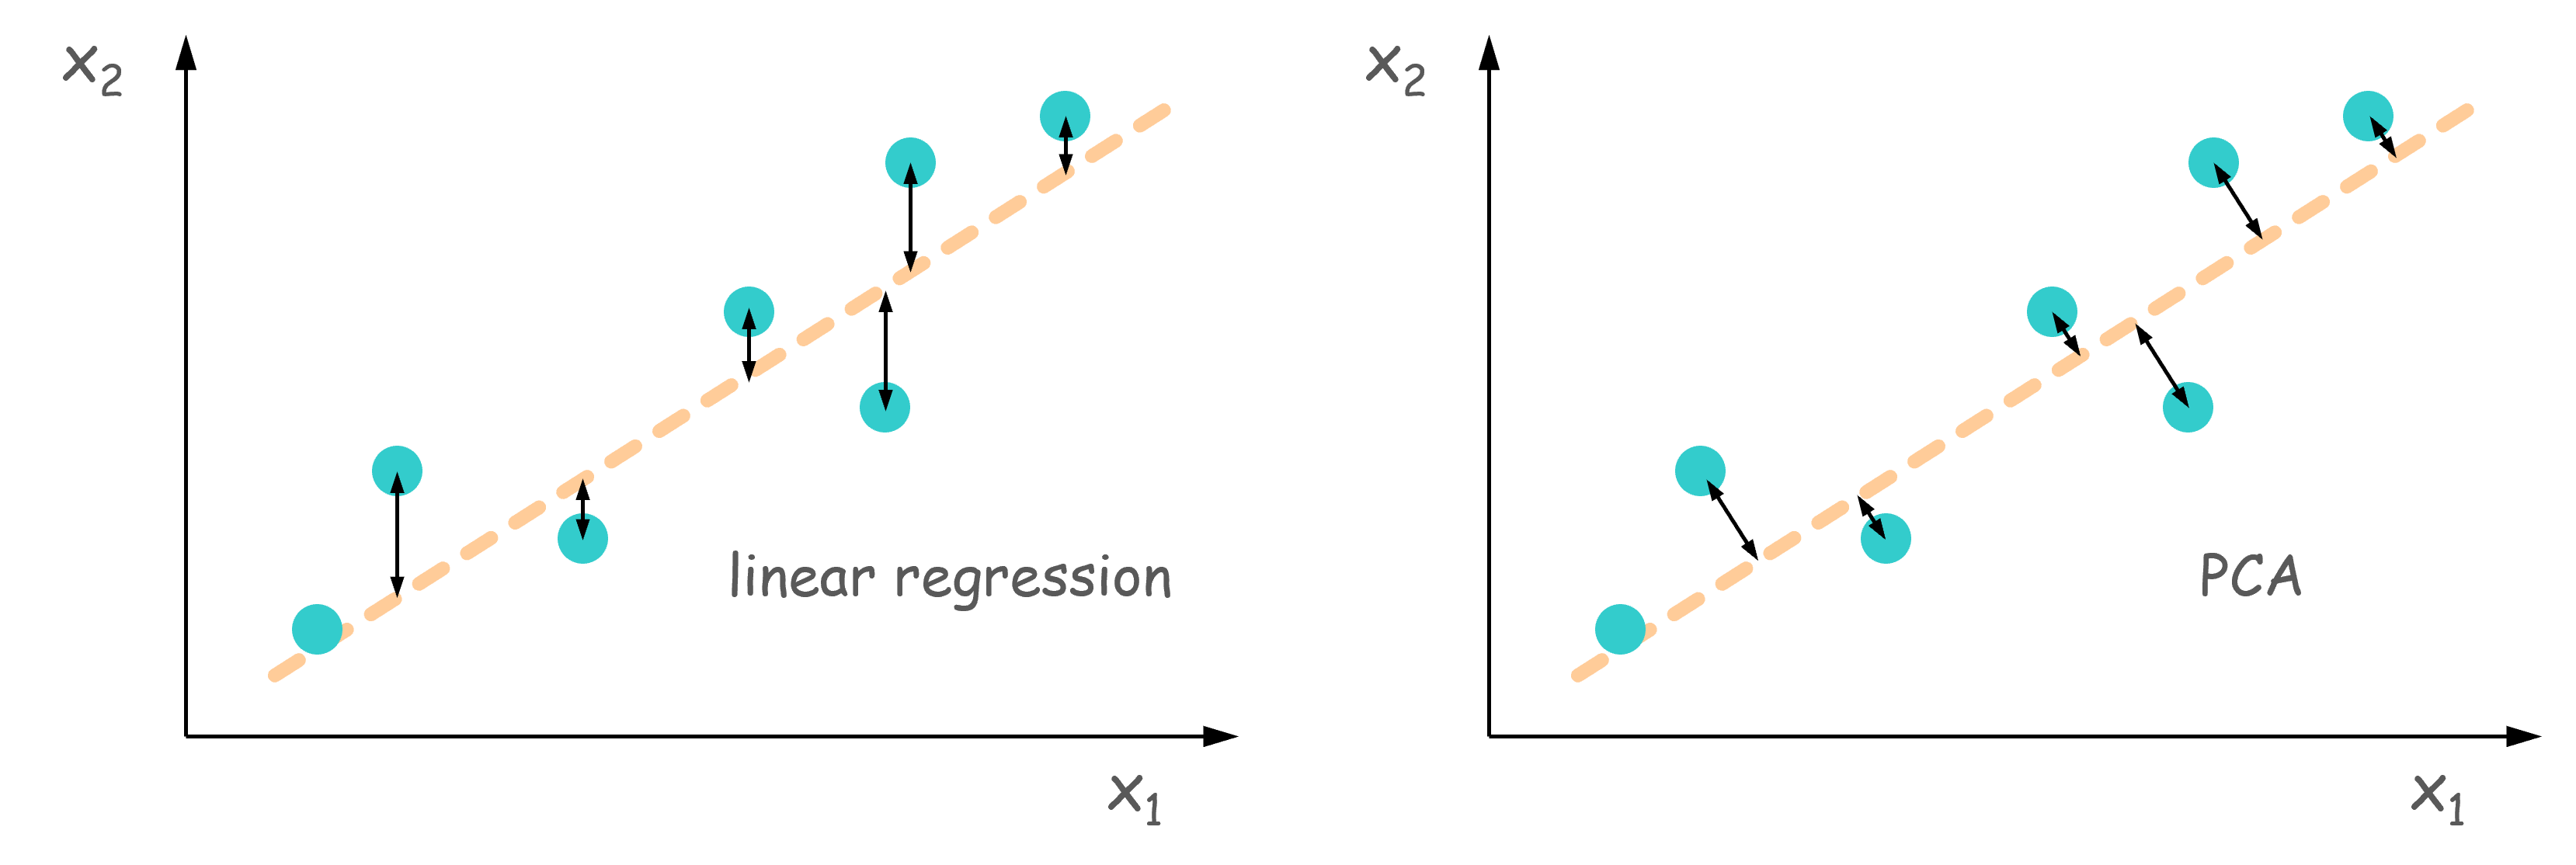
\includegraphics[width=4.4in]{./images/pcaVersusLinearRegression.png}
        \caption{PCA versus linear regression}
    \end{figure}
\end{itemize}


\section{Algorithm}
\begin{enumerate}
    \item Mean normaliza1on and feature scaling
    \begin{equation}
        x^{(i)} \coloneqq \frac{x^{(i)}-\mu^{(i)}}{s^{(i)}}
    \end{equation}
    where $\mu^{(i)}$ is the average of all the values for feature $i$ and $s^{(i)}$ is the range of values, or $s^{(i)}$ is the standard deviation.
    
    \item Compute \emph{covariance matrix}
    \begin{equation}
        \mathbf{C}_{n \times n} = \frac{1}{m}\sum_{i=1}^{m}{ {\mathbf{x}^{(i)}}^T \mathbf{x}^{(i)} } = \frac{1}{m}\mathbf{X}^T \mathbf{X}
    \end{equation}
    
    \item Compute \emph{eigenvectors} by \emph{singular value decomposition}
    \begin{equation}
        \mathbf{C}_{n \times n} = \mathbf{U}_{n \times n} \mathbf{\Sigma}_{n \times n} \mathbf{V}^T_{n \times n}
    \end{equation}
    Here $\mathbf{U}$ is a complex unitary matrix, the columns of which are orthogonal unit vectors called the left singular vectors of $\mathbf{C}$; 
    and $\mathbf{\Sigma}$ is an rectangular diagonal matrix of positive numbers $\sigma\left(k\right)$ called the singular values of $\mathbf{C}$; 
    and $\mathbf{V}$ is a complex unitary matrix whose columns are orthogonal unit vectors either called the right singular vectors of $\mathbf{C}$.

    \item Rearrange the eigenvectors and eigenvalues. 
    Sort the columns of the eigenvector matrix $\mathbf{U}$ and eigenvalue matrix $\mathbf{\Sigma}$ in order of decreasing eigenvalue.
    
    \item Select a subset of the eigenvectors as basis vectors
    \begin{equation}
        \mathbf{U}_{n \times n} = 
        \left[\begin{array}{ccccccc}
             |  &  |  &  |  &       &  |  &       &  |  \\ 
            u_1 & u_2 & u_3 & \dots & u_k & \dots & u_n \\
             |  &  |  &  |  &       &  |  &       &  |  \\ 
        \end{array}\right] = 
        \left[\begin{array}{ccc}
                         &       &  |  \\ 
            \mathbf{U}_k & \dots & u_n \\
                         &       &  |  \\ 
        \end{array}\right]
    \end{equation}
    
    Typically, choose $k$ to be smallest value so that
    \begin{equation}
        \frac{\sum_{i=1}^k \sigma_{ii}}{\sum_{i=1}^m \sigma_{ii}} \geq 0.9
    \end{equation}
    It means $90\%$ of variance retained.

    \item Project the data onto the new basis
    \begin{equation}
        \mathbf{Z}_{m \times k} = \mathbf{X}_{m \times n} \mathbf{U}_{k, n \times k}
    \end{equation}
    
    \item Recover an approximation of the original data that has been reduced to K dimensions
    \begin{equation}
        \mathbf{X}_{m \times n} = \mathbf{Z}_{m \times k} \mathbf{U}_{k, n \times k}^T
    \end{equation}
\end{enumerate}
    \chapter{Anomaly Detection}


\section{Gaussian Distribution}
\begin{itemize}
    \item Say $x \in \mathbb{R}$. If $x$ is a distributed Gaussian with mean $\mu$, variance $\sigma^2$ 
    (where $\sigma$ called ``standard deviation'')

    \begin{equation}
        P(x;\mu,\sigma^2) = \frac{1}{\sqrt{2\pi}\sigma}\exp\left({-\frac{(x-\mu)^2}{2\sigma^2}}\right)
    \end{equation}
    
    \begin{figure}[!htbp]
        \centering
        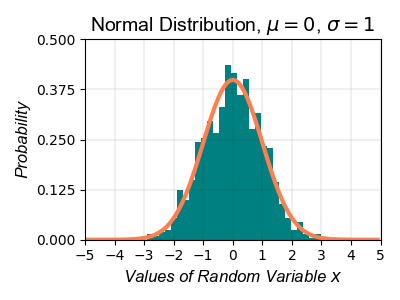
\includegraphics[width=3.2in]{./images/gaussianDistribution.png}
        \caption{Gaussian distribution}
    \end{figure}

    \item Algorithm
    \begin{enumerate}
        \item Choose features $x_i$ that you think might be indicative of anomalous examples, 
        such as ``memory use'', ``CPU load'' for monitoring computers
        
        \item Fit parameters for $\mu_1,\dots,\mu_n$ and $\sigma_1^2,\dots,\sigma_n^2$
        
        \begin{equation}
            \begin{aligned}
                \mu_j      &= \frac{1}{m} \sum_{i=1}^{m}{x^{(i)}_j}\\
                \sigma_j^2 &= \frac{1}{m} \sum_{i=1}^{m}\left(x^{(i)_j} - \mu_j\right)^2
            \end{aligned}
        \end{equation}
        
        \item Compute the probability density function 
        \begin{equation}
            P(x) = \prod_{j=1}^{n} P(x_j;\mu_j,\sigma_j^2) = \prod_{j=1}^{n} \frac{1}{\sqrt{2\pi}\sigma_j}\exp\left({-\frac{(x_j-\mu_j)^2}{2\sigma_j^2}}\right)
        \end{equation}
        
        \item Predict
        \begin{equation}
            y = \left\{
            \begin{array}{llll}
                1 & \text{if} & p(x) <    \varepsilon & \text{(anomaly)}  \\
                0 & \text{if} & p(x) \geq \varepsilon & \text{(nomal)} 
            \end{array}\right.
        \end{equation}
        
        Parameter $\varepsilon$ can be choose by observation from cross validation set.
        There are other ways, such as \emph{error metrices}, \emph{precision/recall} or, \emph{F1 score}.
    \end{enumerate}
    
    \begin{figure}[!htbp]
        \centering
        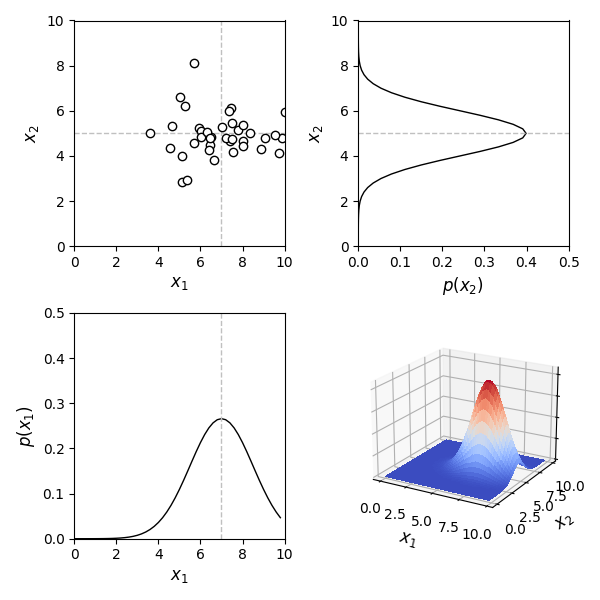
\includegraphics[width=4.2in]{./images/gaussianDistribution_3D.png}
        \caption{Gaussian distribution}
    \end{figure}

\end{itemize}


\section{Multivariate Gaussian Distribution}
\begin{itemize}
    \item The multivariate normal distribution is often used to describe any set of \emph{correlated} random variables.
    If using single-variable distribution to describe a variable-correlated dataset, 
    anomalies could be hard to excluded.
    \begin{figure}[!htbp]
        \centering
        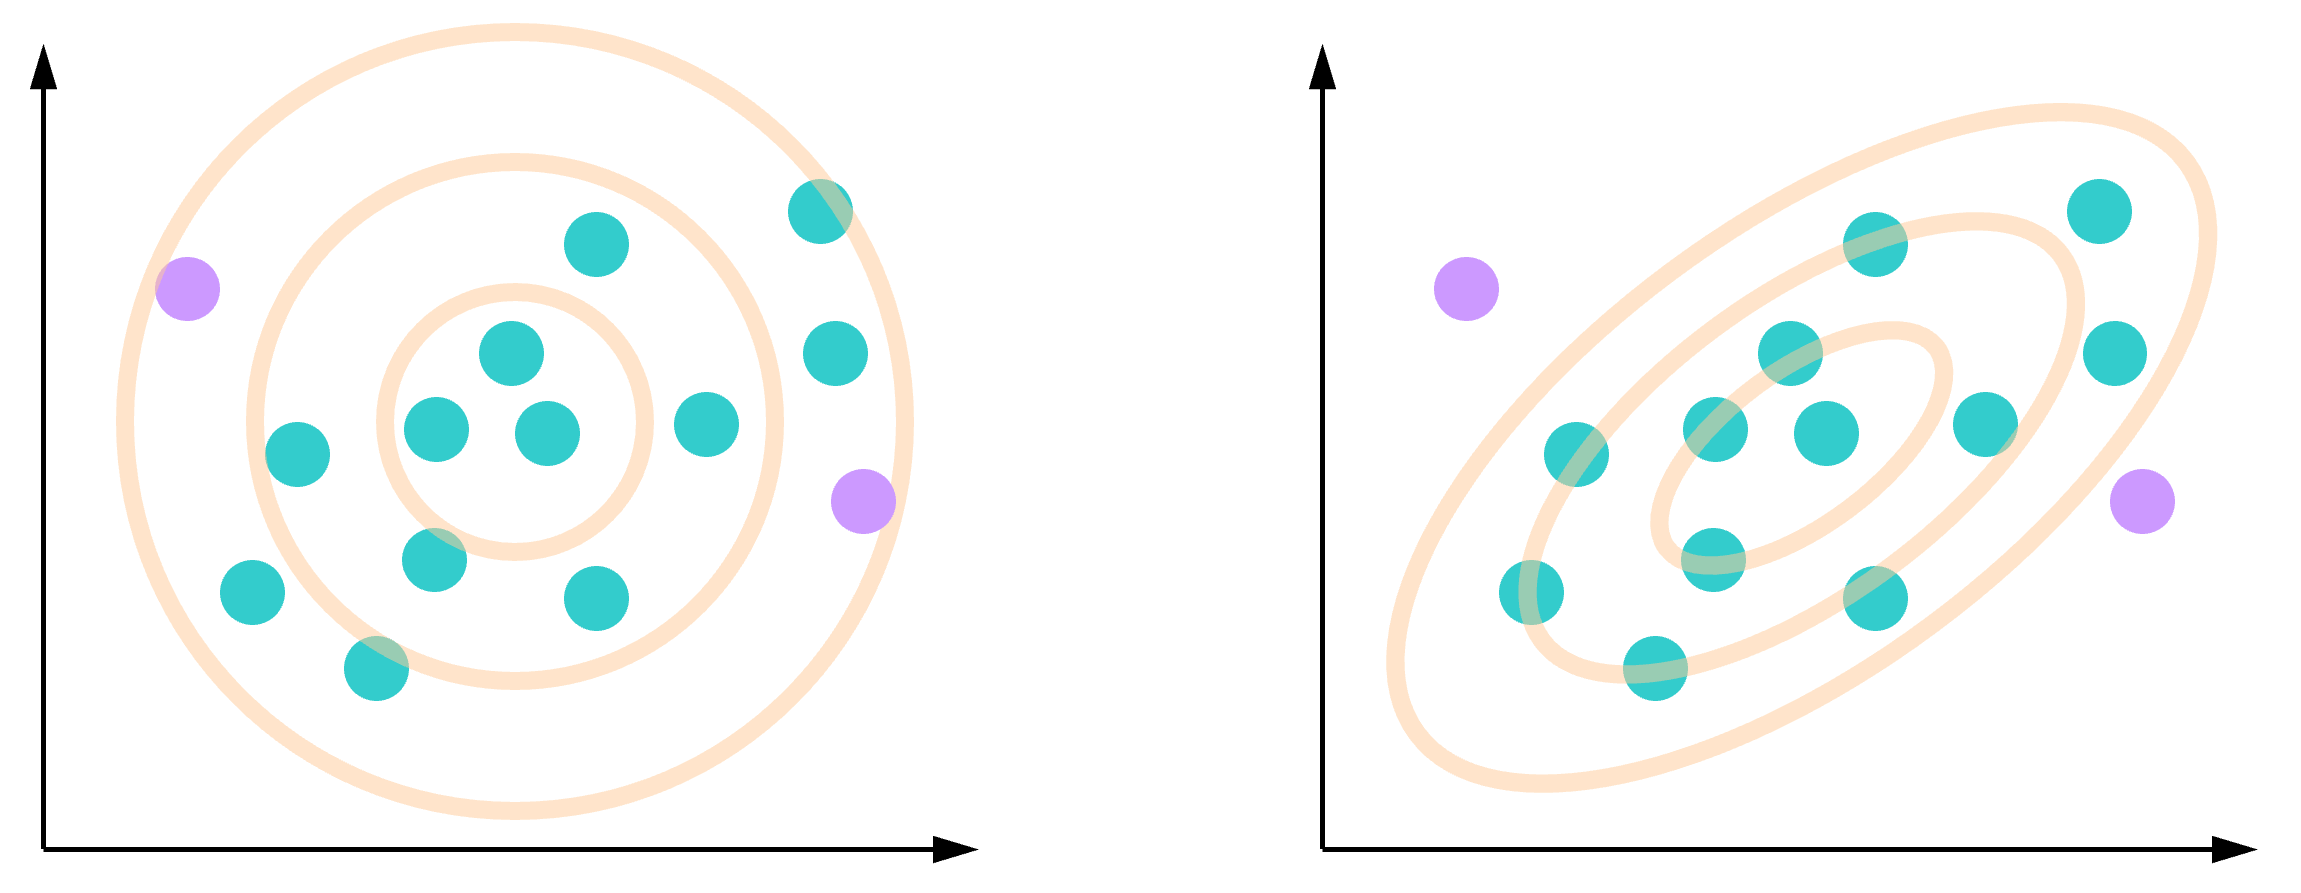
\includegraphics[width=3.6in]{./images/twoDistributionModel.png}
        \caption{Gaussian distribution with single-variate and multivariate}
    \end{figure}
    
    \item Algorithm
    \begin{enumerate}
        \item Fit model $p(x)$ by setting mean vector $\mu\in\mathbb{R}^n$ and covariance matrix $\Sigma\in\mathbb{R}^{n\times n}$
        \begin{equation}
            \begin{aligned}
                \mu    &= \frac{1}{m}\sum_{i=1}^{m} x^{(i)} \\
                \Sigma &= \frac{1}{m}\sum_{i=1}^{m} \left(x^{(i)} - \mu\right) \left(x^{(i)} - \mu\right)^T \\
            \end{aligned}
        \end{equation}

        \item Given a new example $x$, compute probability density function
        \begin{equation}
            p(x; \mu, \Sigma) = \frac{1}{ \left(2\pi\right)^{ \frac{n}{2} } \left|{\Sigma}\right|^{\frac{1}{2}}} \exp{\left(-\frac{1}{2}\left(x-\mu\right)^T\Sigma^{-1}\left(x-\mu\right)\right)}
        \end{equation}

        \item Flag an anomaly if $p(x)<\varepsilon$
    \end{enumerate}

    \item Examples.
    \begin{equation}
        \begin{array}{llll}
        \mu_1 = &\left[\begin{array}{c} 0 \\ 0 \end{array}\right] & \Sigma_1 &= \left[\begin{array}{cc} 1.0 &  0.0 \\  0.0 & 1.0 \end{array}\right] \\
        \mu_2 = &\left[\begin{array}{c} 0 \\ 0 \end{array}\right] & \Sigma_2 &= \left[\begin{array}{cc} 1.0 &  0.5 \\  0.5 & 1.0 \end{array}\right] \\
        \mu_3 = &\left[\begin{array}{c} 0 \\ 0 \end{array}\right] & \Sigma_3 &= \left[\begin{array}{cc} 1.0 & -0.5 \\ -0.5 & 1.0 \end{array}\right]
        \end{array}
    \end{equation}
    \begin{figure}[!htbp]
        \centering
        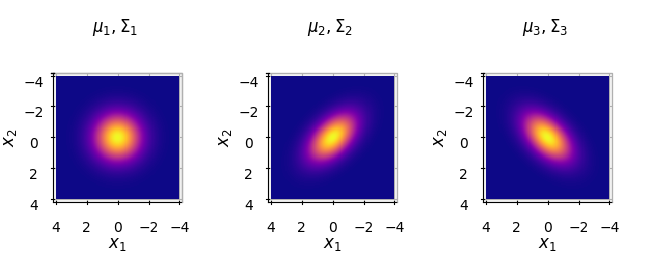
\includegraphics[width=6.2in]{./images/gaussianDistributionMultivariate.png}
        \caption{Gaussian distribution with multivariate}
    \end{figure}

\end{itemize}

    
\section{Non Gaussian Features}
\begin{itemize}
    \item Given the data set that looks like a \emph{log-normal} distribution, 
    take a log transformation of the data, then the histogram looks much more Gaussian.
    
    \item Probability density function for log-normal distribution
    \begin{equation}
        f_X(x) = \frac{1}{x\sigma\sqrt{2\pi}}\exp{\left(-\frac{\left(\ln x - \mu\right)^2}{2\sigma^2}\right)}
    \end{equation}
    
    \item Cumulative distribution function for log-normal distribution
    \begin{equation}
        F_X(x) = \frac{1}{2} \left[1 + \text{erf}\left(\frac{\ln x - \mu}{\sigma \sqrt{2}}\right) \right]
    \end{equation}
    
    \begin{figure}[!htbp]
        \centering
        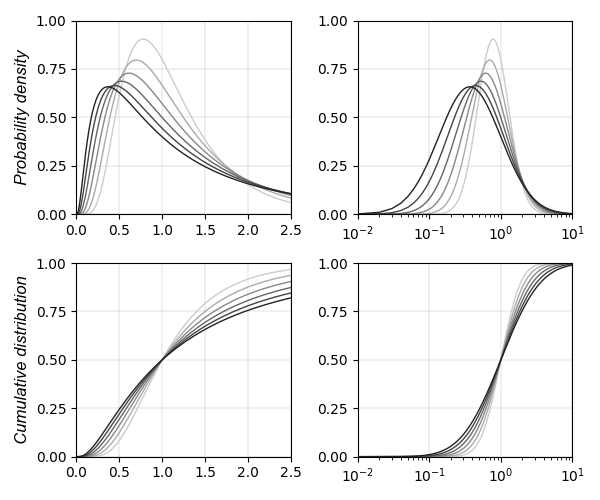
\includegraphics[width=4.2in]{./images/logNormalDistribution.png}
        \caption{Log-normal distribution}
    \end{figure}
    
\end{itemize}


    \chapter{Recommender Systems}
\section{Given Features To Learn Parameters}
\begin{table}[H]
    \caption{Movie ratings}
    \centering
    \begin{tabular}{lcccc}
        \hline %%%%%%%%%%%%%%%%%%%%%%%%%%%%%%%%%%%%%%%%%%%%%
        Movie                & Alice & Bob & Carol & Dave \\ 
        \hline %%%%%%%%%%%%%%%%%%%%%%%%%%%%%%%%%%%%%%%%%%%%%
        Love at last         & 5     & 5   & 0     & 0    \\ 
        Romance forever      & 5     & ?   & ?     & 0    \\ 
        Cute puppies of love & ?     & 4   & 0     & ?    \\ 
        Nonstop car chases   & 0     & 0   & 5     & 4    \\ 
        Swords vs. karate    & 0     & 0   & 5     & ?    \\ 
        \hline %%%%%%%%%%%%%%%%%%%%%%%%%%%%%%%%%%%%%%%%%%%%%
    \end{tabular}
\end{table} 


\begin{table}[H]
    \caption{Movie features}
    \centering
    \begin{tabular}{lcccc}
        \hline %%%%%%%%%%%%%%%%%%%%%%%%%%%%%%
        Movie                & romance & action \\ 
        \hline %%%%%%%%%%%%%%%%%%%%%%%%%%%%%%
        Love at last         & 0.90    & 0.00   \\ 
        Romance forever      & 1.00    & 0.01   \\ 
        Cute puppies of love & 0.99    & 0.00   \\ 
        Nonstop car chases   & 0.10    & 1.00   \\ 
        Swords vs. karate    & 0.00    & 0.90   \\ 
        \hline %%%%%%%%%%%%%%%%%%%%%%%%%%%%%%
    \end{tabular}
\end{table} 


\begin{table}[H]
    \caption{User preference}
    \centering
    \begin{tabular}{lcccc}
        \hline %%%%%%%%%%%%%%%%%%%%%%%%%%%%%%%%%%%%%%%%%%%%%
        Movie       & Alice & Bob & Carol & Dave \\ 
        \hline %%%%%%%%%%%%%%%%%%%%%%%%%%%%%%%%%%%%%%%%%%%%%
        romance     & ?     & ?   & ?     & ?    \\ 
        action      & ?     & ?   & ?     & ?    \\ 
        \hline %%%%%%%%%%%%%%%%%%%%%%%%%%%%%%%%%%%%%%%%%%%%%
    \end{tabular}
\end{table} 


Define
\begin{equation}
    \mathbf{Y} = \left[\begin{array}{cccc} 5 & 5 & 0 & 0 \\ 5 &   &   & 0 \\   & 4 & 0 &   \\ 0 & 0 & 5 & 4 \\ 0 & 0 & 5 &   \\ \end{array}\right], 
    \mathbf{R} = \left[\begin{array}{cccc} 1 & 1 & 1 & 1 \\ 1 & 0 & 0 & 1 \\ 0 & 1 & 1 & 0 \\ 1 & 1 & 1 & 1 \\ 1 & 1 & 1 & 0 \\ \end{array}\right], 
    \mathbf{X} = \left[\begin{array}{ccc} 1 & 0.9 & 0.0 \\ 1 & 1.0 & 0.01 \\ 1 & 0.99 & 0.0 \\ 1 & 0.1 & 1.0 \\ 1 & 0.0 & 0.9 \\ \end{array}\right],
    \mathbf{\Theta} = \left[\begin{array}{cccc} 0 & 0 & 0 & 0 \\ ? & ? & ? & ? \\ ? & ? & ? & ? \\ \end{array}\right]
\end{equation}


Optimize $\theta^{(1)}, \dots, \theta^{(q)}$
\begin{equation}
    \min_{\theta^{(1)}, \dots, \theta^{(q)}} \frac{1}{2}\sum_{j=1}^{q}\sum_{i:r_{ij}=1}\left(x^{(i)}\theta^{(j)} - y_{ij}\right)^2 + \frac{\lambda}{2}\sum_{j=1}^{q} \left\|\theta^{(j)}\right\|^2
\end{equation}


Where
\begin{equation}
    \begin{array}{ll}
        p            &= \text{the number of movies}\\
        q            &= \text{the number of users} \\
        \theta^{(j)} &= \text{column vector for $\mathbf{\Theta}$}\\
        x^{(i)}      &= \text{row vector for $\mathbf{X}$}\\
    \end{array}
\end{equation}


\section{Given Parameters To Learn Features}
\begin{table}[H]
    \caption{Movie ratings}
    \centering
    \begin{tabular}{lcccc}
        \hline %%%%%%%%%%%%%%%%%%%%%%%%%%%%%%%%%%%%%%%%%%%%%
        Movie                & Alice & Bob & Carol & Dave \\ 
        \hline %%%%%%%%%%%%%%%%%%%%%%%%%%%%%%%%%%%%%%%%%%%%%
        Love at last         & 5     & 5   & 0     & 0    \\ 
        Romance forever      & 5     & ?   & ?     & 0    \\ 
        Cute puppies of love & ?     & 4   & 0     & ?    \\ 
        Nonstop car chases   & 0     & 0   & 5     & 4    \\ 
        Swords vs. karate    & 0     & 0   & 5     & ?    \\ 
        \hline %%%%%%%%%%%%%%%%%%%%%%%%%%%%%%%%%%%%%%%%%%%%%
    \end{tabular}
\end{table} 


\begin{table}[H]
    \caption{Movie features}
    \centering
    \begin{tabular}{lcccc}
        \hline %%%%%%%%%%%%%%%%%%%%%%%%%%%%%%
        Movie                & romance & action \\ 
        \hline %%%%%%%%%%%%%%%%%%%%%%%%%%%%%%
        Love at last         & ?    & ?   \\ 
        Romance forever      & ?    & ?   \\ 
        Cute puppies of love & ?    & ?   \\ 
        Nonstop car chases   & ?    & ?   \\ 
        Swords vs. karate    & ?    & ?   \\ 
        \hline %%%%%%%%%%%%%%%%%%%%%%%%%%%%%%
    \end{tabular}
\end{table} 


\begin{table}[H]
    \caption{User preference}
    \centering
    \begin{tabular}{lcccc}
        \hline %%%%%%%%%%%%%%%%%%%%%%%%%%%%%%%%%%%%%%%%%%%%%
        Movie       & Alice & Bob & Carol & Dave \\ 
        \hline %%%%%%%%%%%%%%%%%%%%%%%%%%%%%%%%%%%%%%%%%%%%%
        romance     & 5     & 5   & 0     & 0    \\ 
        action      & 0     & 0   & 5     & 5    \\ 
        \hline %%%%%%%%%%%%%%%%%%%%%%%%%%%%%%%%%%%%%%%%%%%%%
    \end{tabular}
\end{table} 


Define
\begin{equation}
    \mathbf{Y} = \left[\begin{array}{cccc} 5 & 5 & 0 & 0 \\ 5 &   &   & 0 \\   & 4 & 0 &   \\ 0 & 0 & 5 & 4 \\ 0 & 0 & 5 &  \\ \end{array}\right], 
    \mathbf{R} = \left[\begin{array}{cccc} 1 & 1 & 1 & 1 \\ 1 & 0 & 0 & 1 \\ 0 & 1 & 1 & 0 \\ 1 & 1 & 1 & 1 \\ 1 & 1 & 1 & 0 \\ \end{array}\right], 
    \mathbf{X} = \left[\begin{array}{ccc} 1 & ? & ? \\ 1 & ? & ? \\ 1 & ? & ? \\ 1 & ? & ? \\ 1 & ? & ? \\ \end{array}\right],
    \mathbf{\Theta} = \left[\begin{array}{cccc} 0 & 0 & 0 & 0 \\ 5 & 5 & 0 & 0 \\ 0 & 0 & 5 & 5 \\ \end{array}\right]
\end{equation}


Optimize $x^{(1)}, \dots, x^{(p)}$
\begin{equation}
    \min_{x^{(1)}, \dots, x^{(p)}} \frac{1}{2}\sum_{i=1}^{p}\sum_{j:r_{ij}=1}\left(x^{(i)} \theta^{(j)} - y_{ij}\right)^2 + \frac{\lambda}{2}\sum_{i=1}^{p} \left\|x^{(i)}\right\|^2
\end{equation}


Where
\begin{equation}
    \begin{array}{ll}
        p            &= \text{the number of movies}\\
        q            &= \text{the number of users} \\
        \theta^{(j)} &= \text{column vector for $\mathbf{\Theta}$}\\
        x^{(i)}      &= \text{row vector for $\mathbf{X}$}\\
    \end{array}
\end{equation}


\section{Collaborative Filtering Algorithm}
Optimize $\theta^{(1)}, \dots, \theta^{(q)}$ and $x^{(1)}, \dots, x^{(p)}$ simultaneously
\begin{enumerate}
    \item Initialize $\theta^{(1)}, \dots, \theta^{(q)}$ and $x^{(1)}, \dots, x^{(p)}$ to small random values
    \item Compute cost function
    \begin{equation}
        J = \frac{1}{2}\sum_{(i,j):r_{ij}=1}\left(x^{(i)} \theta^{(j)} - y_{ij}\right)^2 + \frac{\lambda}{2}\sum_{j=1}^{q} \left\|\theta^{(j)}\right\|^2 + \frac{\lambda}{2}\sum_{i=1}^{p} \left\|x^{(i)}\right\|^2
    \end{equation}

    \item Minimize cost using gradient descent method
    \begin{equation}
        \begin{aligned}
            x_k^{(i)}      &\coloneqq x_k^{(i)}      - \alpha \left[\sum_{j:r_{ij}=1}\left(x^{(i)} \theta^{(j)} - y_{ij}\right)\theta_k^{(j)} + \lambda x_k^{(i)}     \right]\\
            \theta_k^{(j)} &\coloneqq \theta_k^{(j)} - \alpha \left[\sum_{i:r_{ij}=1}\left(x^{(i)} \theta^{(j)} - y_{ij}\right)x_k^{(i)}      + \lambda\theta_k^{(j)} \right]\\
        \end{aligned}
    \end{equation}

    \item Predict star rating of $\mathbf{X}\mathbf{\Theta}$

\end{enumerate}


\section{Applications}
\begin{itemize}
    \item Finding related movies
    \begin{itemize}
        \item For each product $i$, its feature vector $x^{(i)} \in \mathbb{R}^n$.
        As $\left\|x^{(i)} - x^{(j)}\right\|$ decrease, the similarity between product $i$ and $j$ is increase.
    \end{itemize}

    \item Recommendation for new users
    \begin{equation}
        \mathbf{Y}   = \left[\begin{array}{cccc} 5 & 5 & 0 & 0 \\ 5 &   &   & 0 \\   & 4 & 0 &   \\ 0 & 0 & 5 & 4 \\ 0 & 0 & 5 &  \\ \end{array}\right], 
        \mathbf{\mu} = \left[\begin{array}{c} 2.5 \\ 2.5 \\ 2.0 \\ 2.25 \\ 1.25 \\ \end{array}\right], 
    \end{equation}
    
    Assume the rating by a new user Eve is $\mu$, so the new rating matrix would be
    \begin{equation}
        \mathbf{Y}   = \left[\begin{array}{ccccc} 5 & 5 & 0 & 0 & 2.5 \\ 5 &   &   & 0 & 2.5 \\   & 4 & 0 &  & 2.0 \\ 0 & 0 & 5 & 4 & 2.25\\ 0 & 0 & 5 & & 1.25 \\ \end{array}\right]
    \end{equation}
    
    If mean normalization is a pre-processing step for collaborative filtering
    \begin{equation}
        \bar{\mathbf{Y}} = \mathbf{Y} - \mu = \left[\begin{array}{ccccc} 2.5 & 2.5 & -2.5 & -2.5 & 0\\ 2.5 &   &   & -2.5 & 0\\   & 2.0 & -2.0 &  & 0 \\ -2.25 & -2.25 & 2.75 & 1.75  & 0\\ -1.25 & -1.25 & 3.75 &  & 0 \\ \end{array}\right]
    \end{equation}

    Because the values at the last column of $\bar{\mathbf{Y}}$ are all zeros, it means 
    \begin{equation}
        \theta^{(5)} = \left[\begin{array}{c} 0 \\ 0 \\ 0 \\\end{array}\right]
    \end{equation}
    That implied the preferences of a new user would be neutral.

\end{itemize}



    \appendix

\chapter{Matrices Analysis}
\section{The Gradient Field}
\begin{itemize}
    \item For a scalar function of three independent variables $f(x_{1},x_{2},x_{3})$ the gradient is given by the vector equation
    \begin{equation}
        \begin{split}
            \nabla f = \frac{\partial f}{\partial x_{1}}{\hat {x}}_{1} + \frac{\partial f}{\partial x_{2}}{\hat {x}}_{2} + \frac{\partial f}{\partial x_{3}}{\hat {x}}_{3}\\
        \end{split}
    \end{equation}
    \item This can be seen as the derivative of a scalar with respect to a vector, and its result can be easily collected in vector form
    \begin{equation}
        \nabla f = \frac{\partial f}{\partial\mathbf{x}} = 
        \left(
        \begin{array}{c}
            \frac{\partial f}{\partial x_{1}} \\ 
            \frac{\partial f}{\partial x_{2}} \\ 
            \frac{\partial f}{\partial x_{3}}
        \end{array}
        \right)
    \end{equation}
\end{itemize}            


\section{Inner Products}
Let's proof the inner product of vectors.
\begin{figure}[!htbp]
    \centering
    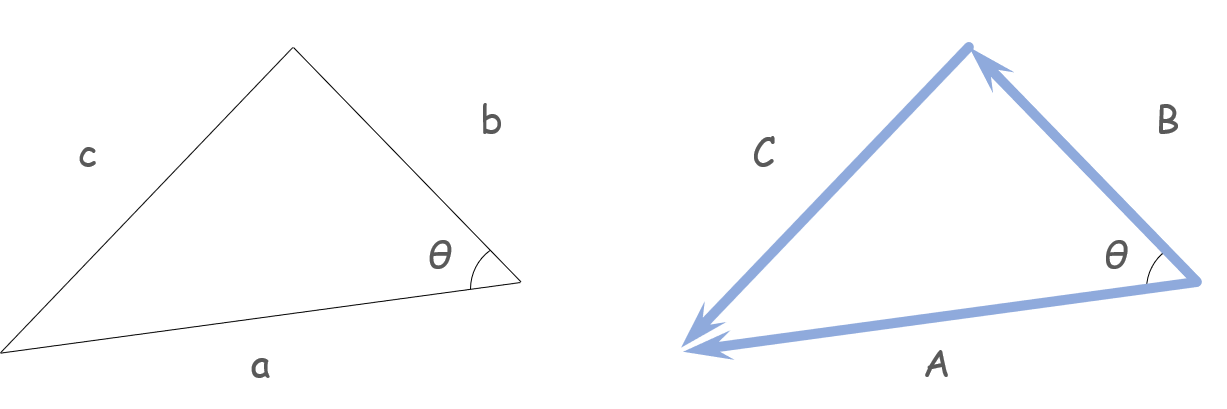
\includegraphics[width=3.6in]{./images/The law of cosine and the angle between vectors.png}
    \caption{The law of cosine and the angle between vectors}
\end{figure}
Recall the law of cosines
\begin{equation} a^2 + b^2 - 2ab\cos\theta = c^2\end{equation}
Apply this to vector triangle
\begin{equation} \left\| \mathbf{A} \right\|^2 + \left\| \mathbf{B} \right\|^2 - 2\left\| \mathbf{A} \right\|\left\| \mathbf{B} \right\|\cos\theta = \left\| \mathbf{A} - \mathbf{B} \right\|^2\end{equation}
Where
\begin{equation} 
    \begin{aligned}
        \left\| \mathbf{A} - \mathbf{B} \right\|^2 &= \left(\mathbf{A}-\mathbf{B}\right) \cdot \left(\mathbf{A}-\mathbf{B}\right) \\
                                                   &= \left\| \mathbf{A} \right\|^2 + \left\| \mathbf{B} \right\|^2 -2\mathbf{A}\cdot\mathbf{B}\\
    \end{aligned}
\end{equation}
This gives
\begin{equation}
    \cos\theta = \frac{\mathbf{A}\cdot\mathbf{B}}{\left\|\mathbf{A}\right\|\left\|\mathbf{B}\right\|}
\end{equation}


\section{Eigenvalues And Eigenvectors}
\begin{itemize}
    \item For a scalar function of three independent variables $f(x_{1},x_{2},x_{3})$ the gradient is given by the vector equation
\end{itemize}            


\section{Singular Value Decomposition}
\begin{itemize}
    \item For a scalar function of three independent variables $f(x_{1},x_{2},x_{3})$ the gradient is given by the vector equation
\end{itemize}            




\chapter{Cheat sheet}
\section{Linear Regression vs Logistic Regression}
\begin{table}[H]
    \renewcommand\arraystretch{1.5}
    \caption{Linear Regression vs Logistic Regression (w/ regularizer)}
    \centering
    \begin{tabular}[t]{lll}     
        \hline 
        \hline 
        Items            & Linear Regression             & Logistic Regression       \\ 
        \hline 
        \hline 
        Cost             & \multirow{2}{*}{$\begin{array}{l} J\left(\theta\right) = \frac{1}{2m} \sum_{i=1}^{m} \left( \mathbf{x}^{(i)}\theta - y^{(i)} \right)^2 \end{array}$}                            & \multirow{2}{*}{$\begin{array}{l} J(\theta) = -\frac{1}{m} \sum_{i=1}^{m} \left[ {y^{(i)}\log{(h^{(i)})}+(1-y^{(i)})\log{(1-h^{(i)})}} \right] \end{array}$} \\
        (original)       &                                                                                                                                                                                 &                                                                                                                                                              \\
        \hline 
        Cost             & \multirow{2}{*}{$\begin{array}{l} J\left(\theta\right) = \frac{1}{2m} \left( \mathbf{X}\theta - \mathbf{y} \right)^T \left( \mathbf{X}\theta - \mathbf{y} \right) \end{array}$} & \multirow{2}{*}{$\begin{array}{l} J(\theta) = -\frac{1}{m} \left( \mathbf{y}^T\log{(\mathbf{h})} + \mathbf{(1-y)}^T\log{(\mathbf{1-h})} \right) \end{array}$}\\ 
        (vectorized)     &                                                                                                                                                                                 &                                                                                                                                                              \\ 
        \hline 
        Gradient descent & \multirow{2}{*}{$\begin{array}{l} \theta_j \coloneqq \theta_j - \frac{\alpha}{m} \sum_{i=1}^{m}\left( h^{(i)} - y^{(i)} \right) x_j^{(i)} \end{array}$}                         & \multirow{2}{*}{Same as linear regression}                                                                                                                   \\
        (original)       &                                                                                                                                                                                 &                                                                                                                                                              \\
        \hline 
        Gradient descent & \multirow{2}{*}{$\begin{array}{l} \theta  \coloneqq \theta - \frac{\alpha}{m}\mathbf{X}^T\left(\mathbf{X}\theta-\mathbf{y}\right) \end{array}$}                                 & \multirow{2}{*}{Same as linear regression}                                                                                                                   \\
        (vectorized)     &                                                                                                                                                                                 &                                                                                                                                                              \\ 
        \hline 
        Normal equation  & $\begin{array}{l} \theta = \left(\mathbf{X}^T\mathbf{X}\right)^{-1}\mathbf{X}^T\mathbf{y} \end{array}$                                                                          & None                                                                                                                                                         \\ 
        \hline
        \hline
    \end{tabular}
\end{table}
\end{document}